\documentclass[11pt]{report}
\usepackage{standalone}
\usepackage{amsmath,amssymb,amsfonts} % Typical maths resource packages
\usepackage{graphicx}                 % Packages to allow inclusion of graphics
\usepackage{color}                    % For creating coloured text and background
\usepackage[table]{xcolor}
\usepackage{hyperref}                 % For creating hyperlinks in cross references
\usepackage{algorithm}
%\usepackage{algorithmic}
\usepackage[noend]{algpseudocode}
\usepackage{longtable}
\usepackage{import}
\usepackage{lscape}
\usepackage{booktabs,colortbl}
\usepackage{tikz}
\usetikzlibrary{patterns}
\usepackage{pgfplots}
\usepackage{pgfplotstable}
\usepackage{endnotes}
\usepackage{cleveref}
\usepackage{caption}
\usepackage{subcaption}
\usepackage{comment}    
\graphicspath{{./img/}}

%\usetikzlibrary{external} 
%\tikzexternalize[prefix=tikz/]
%\tikzset{external/system call={lualatex --shell-escape -halt-on-error -interaction=batchmode -jobname ``\image'' ``\def\tikzexternalrealjob{main}\documentclass[11pt]{report}
\usepackage{standalone}
\usepackage{amsmath,amssymb,amsfonts} % Typical maths resource packages
\usepackage{graphicx}                 % Packages to allow inclusion of graphics
\usepackage{color}                    % For creating coloured text and background
\usepackage[table]{xcolor}
\usepackage{hyperref}                 % For creating hyperlinks in cross references
\usepackage{algorithm}
%\usepackage{algorithmic}
\usepackage[noend]{algpseudocode}
\usepackage{longtable}
\usepackage{import}
\usepackage{lscape}
\usepackage{booktabs,colortbl}
\usepackage{tikz}
\usetikzlibrary{patterns}
\usepackage{pgfplots}
\usepackage{pgfplotstable}
\usepackage{endnotes}
\usepackage{cleveref}
\usepackage{caption}
\usepackage{subcaption}
\usepackage{comment}    
\graphicspath{{./img/}}

%\usetikzlibrary{external} 
%\tikzexternalize[prefix=tikz/]
%\tikzset{external/system call={lualatex --shell-escape -halt-on-error -interaction=batchmode -jobname ``\image'' ``\def\tikzexternalrealjob{main}\input{header}

\title{Computational Models for Risk and Reliability on Bulk Power Systems}
\author{Eric Anderson}% \\
%{\small\em \copyright \  Draft date \today }}
\date{December 10, 2014}

\begin{document}

\include{front}
\include{intro/intro}
\include{msip/msip}
\include{dfo/dfo}
\include{jcc/jcc}
%\include{slk/slk}
\include{back}


\end{document}
''}}
%\tikzset{external/export=false}



%\setlength{\textwidth}{15cm}
\parindent 1cm
\parskip 0.2cm
\topmargin .3cm %1cm  %.3cm
\oddsidemargin .7cm %1.5cm  %.7cm
\evensidemargin .7cm %1.5cm  %.7cm
\textwidth 15cm %13.5cm %15cm
\textheight 21cm %20cm %21cm


\newcommand{\bi}{\begin{itemize}}
\newcommand{\ei}{\end{itemize}}

\newcommand{\norm}[1]{ \left| \left| {#1} \right| \right|}
\newcommand{\magf}{ \left| f \right| }
\newcommand{\magp}{ \left| p \right| }
\newcommand{\magr}{ \left| r \right| }
\newcommand{\magomega}{ \left|  \omega  \right| }
\newcommand{\magE}{ \left| \mathcal{E} \right| }
\newcommand{\magG}{ \left| \mathcal{G} \right| }
\newcommand{\magL}{ \left| \mathcal{L} \right| }
\newcommand{\magM}{ \left| \mathcal{M} \right| }
\newcommand{\magT}{ \left| \mathcal{T} \right| }
\newcommand{\magV}{ \left| \mathcal{V} \right| }

\newcommand{\R}[1]{\mathbb{R}^{#1}}
\def\S{\mathbb{ S}}
\def\I{\mathbb{ I}}


\newcommand{\cA}{\mathcal{A}}
\newcommand{\cB}{\mathcal{B}}
\newcommand{\cD}{\mathcal{D}}
\newcommand{\cCALI}{\mathcal{CALI}}
\newcommand{\cDC}{\mathcal{DC}}
\newcommand{\cGR}{\mathcal{GR}}
\newcommand{\cE}{\mathcal{E}}
\newcommand{\cF}{\mathcal{F}}
\newcommand{\cG}{\mathcal{G}}
\newcommand{\cH}{\mathcal{H}}
\newcommand{\cJ}{\mathcal{J}}
\newcommand{\cK}{\mathcal{K}}
\newcommand{\cL}{\mathcal{L}}
\newcommand{\cM}{\mathcal{M}}
\newcommand{\cN}{\mathcal{N}}
\newcommand{\cO}{\mathcal{O}}
\newcommand{\cS}{\mathcal{S}}
\newcommand{\cT}{\mathcal{T}}
\newcommand{\cU}{\mathcal{U}}
\newcommand{\cV}{\mathcal{V}}
\newcommand{\cW}{\mathcal{W}}
\newcommand{\cX}{\mathcal{X}}


\newcommand{\ry}{\pmb{y}}
\newcommand{\rye}{\pmb{y_e}}


\newcommand{\Expect}{\mathbb{E}}
\newcommand{\Exx}[1]{\mathbb{E}\left[ #1 \right]}
\newcommand{\Var}[1]{Var\left[ #1 \right]}
\newcommand{\CoVar}[2]{CoVar\left[ #1, #2 \right]}
\newcommand{\Prob}{\mathbb{P}}
\newcommand{\cvar}{\mathbb{CV}{\mathsf @}\mathbb{R}}
\newcommand{\grad}{\bigtriangledown}
\newcommand{\lb}{\left\{}
\newcommand{\rb}{\right\}}
\newcommand{\floor}[1]{\lfloor #1 \rfloor}

\newcommand{\defeq}{\stackrel{\rm def}{=}}



\makeatletter
\def\BState{\State\hskip-\ALG@thistlm}
\makeatother


\tikzset{
        hatch distance/.store in=\hatchdistance,
        hatch distance=10pt,
        hatch thickness/.store in=\hatchthickness,
        hatch thickness=2pt
    }

\makeatletter
    \pgfdeclarepatternformonly[\hatchdistance,\hatchthickness]{flexible hatch}
    {\pgfqpoint{0pt}{0pt}}
    {\pgfqpoint{\hatchdistance}{\hatchdistance}}
    {\pgfpoint{\hatchdistance-1pt}{\hatchdistance-1pt}}%
    {
        \pgfsetcolor{\tikz@pattern@color}
        \pgfsetlinewidth{\hatchthickness}
        \pgfpathmoveto{\pgfqpoint{0pt}{0pt}}
        \pgfpathlineto{\pgfqpoint{\hatchdistance}{\hatchdistance}}
        \pgfusepath{stroke}
    }


\usetikzlibrary{arrows,shapes,positioning,shadows,trees,svg.path}

\tikzset{
  basic/.style  = {draw, text width=2cm, drop shadow, font=\sffamily, rectangle},
  root/.style   = {basic, rounded corners=2pt, thin, align=center, fill=green!30, text width=2in},
  level 2/.style = {basic, rounded corners=6pt, thin,align=center, fill=green!45, text width=8em},
  oracle/.style = {basic, rounded corners=6pt, thin, fill=blue!30, text width=10em},
  level 2 oracle/.style = {basic, rounded corners=6pt, thin, fill=blue!10, text width=5.5em},
  level 3/.style = {basic, thin, align=left, fill=pink!60, text width=6.5em}
}


\makeindex


\title{Computational Models for Risk and Reliability on Bulk Power Systems}
\author{Eric Anderson}% \\
%{\small\em \copyright \  Draft date \today }}
\date{December 10, 2014}

\begin{document}

\clearpage\pagenumbering{roman}

\begin{titlepage}
    \begin{center}
        \vspace*{2cm}
        
{\Large        \textbf{Computational Models for Risk and Reliability on Bulk Power Systems}}
                
        \vspace{1.5cm}
        
        \textbf{Eric Anderson}

        \vspace{.2cm}

        December 10, 2014

        \vfill
        
        A preliminary thesis presented to

        \vspace{.25cm}

        Jeff Linderoth\\
        James Luedtke\\
        Bernard Lesieutre \\
        Thomas Rutherford\\
        Stephen Wright

        \vspace{.45cm}

        for partial completion of\\
        Doctor of Philosophy\\
        
        \vspace{0.3cm}
        
        
\includegraphics[width=0.2\textwidth]{uw-madison}
       
        Industrial and Systems Engineering\\        
        University of Wisconsin, Madison\\
        
        \vspace{1.5cm}

        
    \end{center}
\end{titlepage}



 \addcontentsline{toc}{chapter}{Contents}
\setcounter{tocdepth}{2}

\tableofcontents

\listoffigures
\listoftables

\clearpage\pagenumbering{arabic}

\newcommand{\mypath}{../thesis}
\newcommand{\mypathintro}{../thesis/intro}
\chapter{Introduction}\label{intro-chapter}
This thesis focuses on reliability issues for the electricity grid that powers the United States.  Electricity is a critical service used by almost every person and company within our country.  Reliability issues cost industry billions of dollars every year.  Large scale power outages are national disasters due to the loss of services such as cell phones, city wide water pumping, gasoline stations, trains, subways, and cooling which inevitably lead to economic loss and loss of life.  

The introduction starts with an overview of the electrical infrastructure of the United States.  Following are the basics of how the power system operates on a day-to-day basis and the organizational structure that operates it. Then, the events of August 2003 are explained where part of the Northeast electricity grid collapsed in a cascading power failure leading to millions of people without power, billions in economic loss and the loss of life.  This is just one example of a large scale power outage, which is rare, but extremely costly to society. After this, general reliability issues of the power grid is discussed which cost society billions annually.
 
After defining the problem, this thesis explains the tools and methodology for attempting to make our system more robust against such failures.  First, the current literature on cascading power failures is explored.  This is used to model the cascading process as a multi-stage stochastic program with mixed-integer decision variables.  It is shown to have a similar distribution to the simulation, however is computationally difficult.  We turn to optimizing design problems with the cascading simulation as a subproblem.  This allows us to take advantage of accessory information in the cascading simulation as well as parallelize the computational effort to solve large scale problems in  a timely manner.  Finally, a system risk measure is developed to control endogenous, congestion based line failure risk.  This risk measure is used in a real time dispatch model with net injection uncertainty and the cost-risk frontier is explored.

%First, a model of the cascading process is made.  This model captures the effects of the cascading process while remaining simple enough to solve in a reasonable time.  After a model is developed, design problems are formulated in order to improve either the infrastructure or the operation of the system.  These design problems fit into broad families of optimization problems.  Algorithms for these types of problems are used and modified for our particular problem.  Finally, with the help of computation resources, solutions are found to these design problems in order to gain insight into the problem and help protect our system from potential future outages.

\section{Power Systems Introduction}
The United States electrical infrastructure is a complex physical structure which connects the consumers of electricity with generating assets over a large geographic area.  The nature of electricity makes the operation of this infrastructure extremely difficult and is accomplished through numerous organizations and people working together to supply electricity at the least cost while maintaining a given level of reliability.

	As of 2004, the electrical infrastructure was comprised of more than \$1 trillion in asset value.  This includes over 200,000 miles of high voltage transmission lines, 950,000 MW of generation, and 3500 utility organizations serving 283 million people \cite{northeast_2003}.  The introduction briefly looks at generation and the transmission system which efficiently moves the energy over long distances.

\subsubsection{Electricity Generation}
	Electricity is generated using a variety of fuels and procceses.  The most common method of electricity generation creates steam by heating water, which spins a turbine producing an alternating current of electricity.  The United States operates its power grid at 60 hz, that is, the direction of electrical flow switches 60 times every second.  Since the generators are tied to the grid, when the grid is stable, the generators are rotating synchronously with the power grid.  The water can be heated by different fuels such as coal, natural gas, fissioning heavy elements such as uranium, or even using geothermal temperature differentials.  The Rankine cycle is a model of converting heat into mechanical energy for steam engines.  The efficiency of the cycle is limited by the difference between the turbine entry temperature and the condenser temperature.  This means that steam cycle power plants need an external cooling source which removes the waste heat from the working fluid before it begins the cycle again.  

	The first example of a steam cycle power plant is a coal plant.  The chemical energy in coal is converted into thermal energy and byproducts such as carbon dioxide.  Power from coal provides around 40\% (for the year 2013 \cite{eia_gov}) of the electricitty generation in the United States. These plants have more thermal inertia which makes changing the output level a slow process.  Modern coal plants achieve efficiencies of 30-40\%, that is, the percentage of their input energy which is injected into the grid as electricity is 30-40\%.

	Nuclear power plants (19\% of electricity) also operate on the steam cycle, producing heat by fissioning heavy elements such as Uranium-235.  Nuclear plants have relatively slow ramping rates and cheap fuel, which lead them to be dispatched at high output rates continuously.  These plants, along with coal plants, provide the majority of baseload power production. Baseload power is the minimum amount of power that needs to be produced continuously throughout the day.  Nuclear fuel has a desirable aspect of being extremely energy dense.  The energy density of Uranium-235 is roughly 3 million times denser than coal.  This means that the waste products of this process are much less than other types of power plants and are also captured completely without being released to the environment.

	Natural gas plants (27\% of electricity) can capture, in addition to the heat energy, the combustion energy and use it to spin a gas turbine.  Gas turbines, while having a lower thermal efficiency, have the desirable trait to quickly throttle production to the desired level in contrast with steam cycles.  Additionally, by using a combination of both combustion and heat energy, combined-cycle natural gas plants can reach efficiencies of around 60\%.  These fast ramping rates and more expensive fuel lead natural gas plants to provide peaking power matching electrical demand over baseload.  Recently, with relatively cheaper natural gas and increased efficiencies from combined-cycle plants, natural gas plants are playing more of a role in electrical demand between baseload and peaking levels.    

	Hydroelectric power (6\% of electricity) has many desirable traits and it is the largest source of renewable energy generation installed around the world.  By creating a reservoir to hold a large amount of water at a high level, potential energy can be stored.  When this water is released, it becomes kinetic energy, which can be captured by a turbine and used to generate electricity.  By controlling the flow into the turbine or the amount of turbines spinning, hydro power is capable of not only storing energy, but also quickly adjusting its output rate.  However, they have the additional constraint of needing to maintain given reservoir levels throughout the year.

	In the past decade, we have introduced a sizeable amount of electricity production from renewable sources such as wind turbines and solar panels (both total 6\% of electricity, with wind comprising the majority).  These generation sources have a cheap fuel (kinetic energy from the wind and solar radiation), but are unable to control output.  

	The different characteristics of generators give each a different roles to play in the operation of the power system in order to meet demand.  These various generation assets are owned by utilities, independent power producers, large industrial customers themselves, and, more recently, residential consumers.  

\subsubsection{Transmission Network}
	The production from the majority of large generation plants is at lower voltages (10kV - 25kV).  Electricity traveling in transmission elements lose energy due to resistive losses, which primarily goes into heating up the power line.  The resistive losses are proportional to the current.  In order to reduce losses, the voltages are stepped up to between 230 kV to 765kV for long distance transmission elements, which has the effect of reducing the current for a given amount of power.  At the demand side, there are radial tree-like distribution networks operating at low voltages (less than 1kV) which connect every demand node to the power grid.  The United States power grid is broken into three distinct power grids: Western Interconnection, Eastern Interconnection, and Texas Interconnection. Each has a network of transmission lines connecting all of the generators with all of the loads.  

	Power flows, according to the laws of physics, along ``paths of least resistance", which are modeled with Kirchoff Voltage Laws (KVL) and Kirchoff Current Laws (KCL).  This means that electricity flow can't be controlled like many other complex networks such as cell phone and internet traffic, but instead follows laws of physics much like water or gas in pipe networks.  In addition, electricity flows at close to the speed of light and currently is hard to store economically, unlike water and gas.   There needs to be an instantaneous balance of generation and demand.  

\subsubsection{Organizational Structure}
The primary reliability organization which develops operating and planning standards is North American Reliability Council (NERC) and ten regional councils. 
\begin{description}
\item[NERC] develops standards for reliable operation and planning of the bulk electric system and then monitors and assesses compliance.  Also, they provide education and training, while coordinating critical infrastructure protection, such as information exchange between reliability service organizations.  Finally, they assess, analyze, and report performance and system adequacy.
\end{description}
 The primary focus of the reliability and planning standards is to be able to serve all demand reliability both today and in the future.  There are 7 primary tasks:
\begin{itemize}
\item Balance power generation and demand continuously;
\item Balance reactive power supply and demand to maintain scheduled voltages;
\item Monitor flows over transmission lines and other facilities to ensure thermal limits not exceeded;
\item Keep system in stable condition;
\item Operate so that it remains in reliable condition even if contingency occurs (N-1 critiera) and when a contingency does occur, maneuver to new stable N-1 position. The N-1 criteria states that the system must be robust against any single component of the power grid failing;
\item Plan, design, and maintain the system to operate reliably; and
\item Prepare for emergencies.
\end{itemize}

Within the United States, Federal Energy Regulatory Commission (FERC) is the federal agency with control over electricity sales, natural gas and oil pipelines, and hydropower projects and has increased power after the  Energy Policy Act of 2005.  This differentiates it from NERC in that it can impose mandatory standards.

\begin{description}
\item[FERC] imposes mandatory reliability standards for the bulk transmission system and imposes penalties on those that manipulate the markets.  Its primary tasks are the following:
\end{description}
\begin{itemize}
\item Regulate transmission and wholesale electricity sales in interstate commerce;
\item License non-federal hydroelectric projects;
\item Ensure reliability of high voltage interstate transmission system;
\item Monitor and investigate energy markets;
\item Penalize violating entities, through civil penalties or other means; and
\item Oversee environmental matters relating to major policy initiatives.
\end{itemize}

The restructuring of the power grid has decoupled utilities from the responsibility of maintaining a control area.  The 140 control areas are operated by the 10 regional Independent System Operators (ISOs) or Regional Transmission Organizations (RTOs).  
\begin{description}
\item[ISO/RTO] are tasked with providing least cost energy to everyone within its territory while maintaining a given level of reliability.  In order to do this, they create wholesale electricity markets in order to balance generation and load in real time at least cost.  Their tasks are the following:
\end{description}
\begin{itemize}
\item Manage the wholesale electricity markets while maintaining the reliability of the system; 
\item Direct the operation of the assets owned by their members; and
\item Encompass multiple control areas within the territory that they operate.
\end{itemize}

\subsubsection{Wholesale Electricity Markets}
The ISO or RTO use 3 primary markets for determining how much each generator should produce at any given time.  The first market is bi-lateral contracts.  These are long term contracts between producers and suppliers to exchange a certain quantity of energy at a given price.  These contracts help provide reliable, long term forecasting for supply and load. This reduces exposure to the volatility of the day ahead and real time markets.  

The day ahead market takes bids from generators which contain an array of costs to produce a certain amount of electricity.  The generators also provide additional operational constraints, such as ramping rates and start-up and shut-down times and costs.  In addition to generators' physical constraints, forecasts for demand of the following day is used to get an estimate of the amount of generation needed.  Using the transmission constraints for the given network, the ISO clears this market during the previous day.  This process usually takes around four hours and is done with specialized optimization tools solving the optimal power flow problem with security constraints and unit commitment decision variables.  The outcome of this process is the schedule for slow ramping generators and hourly locational marginal prices (LMP) at each location in the network for the following day.  These prices are guaranteed and any deviation from the schedule are made up in the real-time market.	

The real-time market makes up for errors in forecasting as well as possible failures in generation or transmission.  This market operates on five minute intervals and can be extremely volatile.  Similar methods as the day-ahead are used to clear this market, although simplified due to the time constraint.  Price spikes can occur during times of peak demand and a congested grid in which the price of electricity can often become over 10-20 times as expensive.  The reverse is also possible.  During times of low demand, it is possible for negative prices on the real time market.  This occurs because the generators are constrained by ramping rates and there is too much production on the grid. In \cref{fig:lmpmiso}, there are negative prices across the Midwest and, in particular, Iowa, with much higher prices in Illinois.  This LMP snapshot is taken at night when there is low demand for electricity as well as increased production from wind farms located in the Midwest.  The differences in prices suggest significant transmission bottleneck constraints between the Upper Midwest and Illinois.   


\begin{figure}
\centering
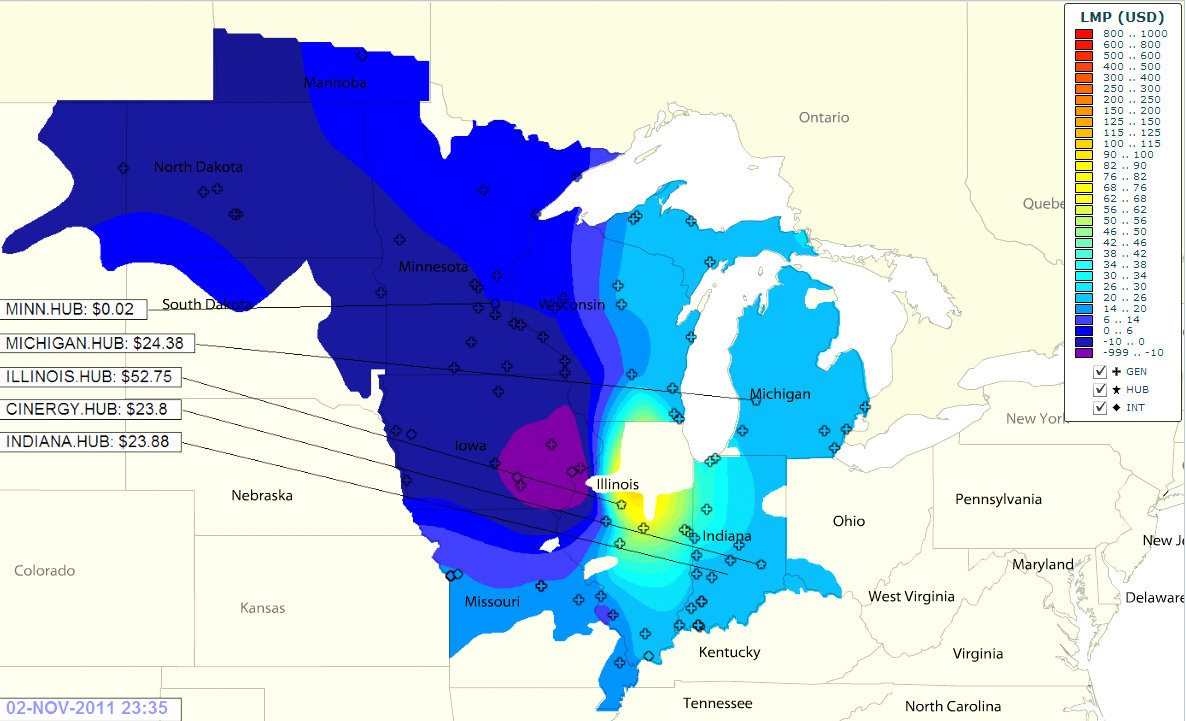
\includegraphics[width=5in]{lmp}  
\caption{Location Marginal Prices (LMP) for Midwest ISO's territory}
\label{fig:lmpmiso}
\end{figure}


\subsubsection{Operating Constraints}

In order for the power grid to operate and maintain stability, a number of things must hold.  First and foremost, there must be a continuous balance of power generation and demand.  The US grids are all operated with a target frequency of 60 hz, but the actual system frequency varies.  When there is excess generation on the grid, the frequency will increase and with a lack of generation, frequency will drop.  Since the generators are synchronized with the grid, when the frequency deviates from normal, the generators can move out of their operating limits and cause damage.  Generators have internal protections to identify bad operating points and trip offline in order to protect themselves.  In order to protect the grid, there is automated tripping of load at certain frequency points to take customers offline and prevent total collapse.  

In addition to real power balance, reactive power supply and demand must be used to maintain scheduled voltages.  Low voltage can cause system instability and damage to motors and electrical equipment.  Also, high voltage can exceed insulation capability and cause dangerous arcs.  Reactive power is supplied through capacitor banks and generator output.

In order to protect the transmission elements, the flows over transmission lines and other facilities must be monitored to ensure thermal limits are not exceeded.  Lines are heated by electricity flow and equipment can be damaged, such as conductors sagging from stretch and expansion due to high temperatures.  These problems are affected by ambient temperature and wind conditions.  The flow is limited so the line does not sag into obstructions such as trees and telephones.



\section{Cascading Power Failures}
A cascading power failure is a set of failures of individual components of the transmission system which leads to the redistribution of power over the new topology.
 When the system is in a stable operating position, individual components often have a negligible effect on system-wide distribution.  However, after several failures, the transmission network may not have enough capacity to distribute the power from the generation to the load.  This can cause a series of fast acting trips in which a large portion of the grid may fail.  While rare, these events are extremely costly.


\subsection{Northeast 2003 Blackout} 

%This account of the Northeast Blackout is drawn from the \textit{Final Report on the August 14, 2003 Blackout in the United States and Canada} by the U.S.-Canada Power System Outage Task Force.\cite{northeast_2003}  

\subsubsection{Historical Problems}
The Northeast blackout of 2003 began in the Cleveland-Akron area of the Eastern Interconnection.  This area had a history of problems of low voltages due to the relatively high amount of imported power.  In 1998, the system was becoming unstable and everything other than load shed was done to fix the problem.  It was shown to not be within the reliability standards, and regulations were loosened instead of addressing the problem.  A transformer problem led American Electric Power (AEP), a control area entity, to perform a reliability study on the neighboring control area operated by First Energy (FE).  The study again showed voltage instability problems.

The summer of 2003 was fairly typical with less than historical peak load.  While the load was less than historal peak, it was consistently greater than the forecasted load.  High temperatures, creating a greater air conditioning load, contributed to reactive power shortages.  The voltages were low in Cleveland-Akron during the week, but within the new operating limits (92\% to 105\%).  A group of shunt capacitors, out of service for planned maintenance, further reduced reactive power supply.  Also, a large nuclear reactor, Davis-Besse, was in a long term forced outage state.  This plant is normally able to provide a large amount of real power as well as reactive power support.

\subsubsection{Normal Day Turns Bad}
A series of initiating events, as well as the failure of FE's control server, led to an unstable system and the inability for operators to do anything about it.  In addition, neighboring regional reliability coordinators (Midwest Independent System Operator, MISO, and Pennsylvania-New Jersey-Maryland Interconnect, PJM) had bad information on the state of the system and were unable to provide support.  The operators had concern about voltage levels and were trying to get additional reactive power online.  The shunt capacitors were unable to return to operation.

The following initiating events didn't cause the system to collapse, but moved it into an unreliable state, which allowed the collapse to take place. The Stuart-Atlanta 345 kV line tripped due to contact with surrounding vegetation (area voltage at 98.5\%) at less than 100\% capacity.  In addition to the loss of the line, MISO was unaware, which led to unusable output and the inability to provide support.  An important generating unit, Eastlake 5, attempts to increase reactive power output, but the internal protection trips the generator offline (area voltage 97.3\%).  This led to real power imports rising, which increased the need for reactive power as well.  Another transmission line loss of Harding-Chamberlin 345 kV continued to depress the voltage (95.9\%).  Around this time, the underlying 138 kV network began to fail.   MISO was unable to perform N-1 contingency analysis and the FE reliability charts flatlined due to the server problems.

Ultimately, it was in reliable state before 15:05, however, after all of these events, the system was no longer N-1 stable.  In addition, reliability coordinators were using separate state information due to poor communication.  

\subsubsection{System Becomes Unreliable}

A total of 3 lines tripped at below operating capacity due to tree contact starting with Harding-Chamberlin (44\% of capacity) at 15:05.  Then the Hanna-Juniper line tripped (88\% normal and emergency rating) at 15:32.  The Star-South Canton line had multiple tree contacts (55\%) starting at 14:27, and finally tripped off for good (93\% emergency rating)  at 15:41.  There were no prior sustained outages from tree contact in the previous years and FE used vegetation management practices consistent with the industry.  When designing line limits, the thermal ratings are based on many variables including ambient temperatures and wind speeds.  A combination of higher than nominal ambient temperature and lower wind speeds reduced the cooling capacity of lines.

Perry plant, the largest local generator, was getting voltage spikes at levels close to tripping the generator.  They notified FE of the problems, but the operators were unable to recover from this precarious situation.  The task force notes that load shed here of 1500MW may have saved the system by increasing voltages and stopping the ultimate trip of Sammis Star line.

\subsubsection{High Speed Cascading Failures}
At 16:05 the final straw was pulled by the tripping of the Sammis-Star 345kV line separating geographical regions of the grid.  Unplanned power shifts across regions caused phase 3 operations in the protective relays of transmission elements, which can trip lines far away from the problem area.  The grid continued to stabilize after each one of these individual outages.  However, by 16:10, the north and south separated (AEP separates from FE), and the high generation area was no longer directly connected to the high load center.  This caused a massive power surge from PJM through New York and Ontario counter clockwise around the great lake to load centers in Michigan. This surge caused the Northeast to separate from the rest of Eastern Interconnect (EI).

There was insufficient generation in the newly formed islands to support the load.  The frequency in remaining parts of EI rose to 60.3\%, representing 3700 MW of excess generation.  The Northeast grid kept breaking apart until islands were formed in which an equilibrium between load and generation could be made.  Under-frequency and under-voltage load shedding helped to stabilize the system within the islands.  New York dropped 10,648 MW through automatic load shedding and Ontario dropped 7800 MW.  Some generators tripped off at unreasonable levels making island stabilization more difficult.  Thousands of events occured between 16:10 and 16:13.  

The cascade spread, not due to voltage problems, but dyanmic power swings which caused system instability.  The voltage instability was only companion to the angle instability (represents large real power flow swings) which tripped generators and lines.  The large power swings come from imbalance between generation and load across regions and the electrical separation of these two areas.  The inherent weak points are lines with the highest impedence, which trip off relatively early due to protective relay settings.  These are typically long over-head lines with high loadings.


\subsubsection{The Blackout Results}
In the United States, 45 million people lost power totaling 61,800 MW in Ohio, Michigan, Pennsylvania, New York, Vermont, Massachusetts, Connecticut, and New Jersey.  The US loss estimate was between \$4 billion and \$10 billion.  Another 10 million people from Canada lost power leading to an estimated 18.9 million lost man hours and \$2.3 billion in lost manufacturing shipments.   There were at least 11 fatalities, power took up to 4 days to return, and rolling blackouts continued in Ontario for the following week.\cite{northeast_2003}

The formation of a large island, based off of hydro plants in western New York and Canada, was the basis for system restoration.
 

\section{Reliability in Power Systems}
The electricity grid is held to a higher reliability standard than other services since it is critical infrastructure for society.  Even though the power system maintains a very high level of reliability, power interruptions still have large costs to consumers.  After a discussion of the economic costs, the trends in power outages for the North American grid are looked at.

The economic loss caused by power interruptions to electricity consumers in the United States for 2001 was estimated at \$79 billion \cite{lacommare_2006}.  This can be compared to the total revenue of electrical sales in the year 2001 of \$247 billion \cite{eia_sales}.  The single event of the Northeast blackout in 2003 was estimated to have a total impact on US workers, consumers, and taxpayers as a loss of approximately \$6.4 billion \cite{anderson_2003}.  This cost is hidden from the system, but may entertain the notion that the true cost of electricity is higher than the current prices.  

The current power system has evolved throughout the last century due to economic and reliability issues and the responses of the operating entities to these forces.  The power system has self-organized into a dynamic equilibrium where blackouts of all sizes occur \cite{dobson_2001}.  The average frequency of blackouts in the United States is 13 days and has been the same for 30 years \cite{carreras_2004}, which represents this equilibrium.  
	
NERC data shows that distribution of blackouts for the last 15 years (1988-2003) follows a power tail curve with an exponent of around $-1.3\pm.2$ \cite{carreras_2004}. This is strengthened further where Hines {\it et. al.} showed that the frequency of blackouts in the United States is not decreasing, changes seasonally and with the time of day, and follows a power-law distribution \cite{hines_2008,hines_2009}.

Some emerging conditions on the grid may make protection more important and more difficult, shown in \cref{tab:change1}.  Electric vehicles adopted en masse have a potential to offer useful services to the power grid through the use of a sizable amount of energy storage in aggregate.  However, they also represent a considerable stress on the system in different spots and ways than it is used to.  The ideal car battery system would have a quick charge, that is, the ability to transfer the energy from the grid to the battery extremely quickly.  This would allow consumers to use charging stations similar to the current gasoline stations for combustion engines.  A charging station capable of charging many cars would have extremely high and unpredictable volatility that the system needs to protect against.

The increased penetration of renewable energy production also increases stress on the power system.  Wind and solar are both variable generation devices which do not actively control the amount of electricity being produced.  The system needs to maintain ample ramping capability in order to maintain stability.  These stresses can be reduced by improving the quality of forecasting efforts on various timescales.  In addition, these technologies are geographically constrained by their fuel source availability, wind speeds and solar irradition.  However, these natural fuel sources do not align with large demand centers, so the transmission system is needed to efficiently distribute the energy produced.

\begin{table}
\centering
\footnotesize
\begin{tabular}{| p{7cm} | p{7cm} |}
\hline
\bf Previous Conditions 	&	\bf Emerging Conditions 		\\	\hline  	\hline
Fewer, relatively large resources	&	Smaller, more numerous resources		\\	\hline
Long-term, firm contracts 	&	Contracts shorter in duration, more non-firm transactions, fewer long-term firm transactions	\\	\hline
Bulk power transactions relatively stable and predictable	&	Bulk power transactions relatively variable and less predictable	\\	\hline
Assessment of system reliability made from stable base (narrower, more predictable range of potential operating states)	&	Assessment of system reliability made from variable base (wider, less predictable range of potential operating states)		\\		\hline
Limited and knowledgeable set of utility players 	&	More players making more transactions, some with less interconnected operation experience; increasing with retail access	\\	\hline
Unused transmission capacity and high security margins	&	High transmission utilization and operation closer to security limits	\\	\hline
Limited competition, little incentive for reducing reliability investments	&	Utilities less willing to make investments in transmission reliability that do not increase revenues	\\	\hline
Market rules and reliability rules developed together	&	Market rules undergoing transition, reliability rules developed separately	\\	\hline
Limited wheeling	&	More system throughput	\\	\hline
\end{tabular}
\caption{\small Changing conditions that affect system reliability (from the Northeast outage report \cite{northeast_2003}).}
 \label{tab:change1}
\end{table}

\section{Thesis Roadmap}
% The themes in this research

In this thesis, we work to evaluate and reduce the likelihood and effects of rare event failures on the bulk power system.  We start by reviewing the current literature on cascading power failures and we use a cascading simulation common in literature to build upon. We first formulate this as a large, multi-stage stochastic program using binary variables to model line failures and an effective capacity distribution to model decision dependent uncertainty.  Then, we decompose this model by scenario in order to get an efficient and parallelizable cascade simulation.  We look at transmission expansion and optimize over this long term design problem using derivative free optimization techniques.  Then, we look at line failures in the five minute time horizon and develop a dispatch model to constrain the likelihood of line failures over this time frame.  We extend this model to the N-1 exogenous contingencies and combine it with the OPA model to evaluate and constrain rare event risk.

The cascading power failure simulation we use, and is used in other literature, can be seen as an empirical model in which the distribution of load shed from these events follow the same power-law distribution that is seen in the real world.  It uses topology information as well as linearized power flow constraints that are necessary to capture some of the important effects of power system operation.  This model does not attempt to capture short term transients involved in the physical evolution of these cascading processes.  Instead, it attempts to capture the distribution of possible outcomes and evaluate the system risk associated with rare events.

We have three primary themes and areas of contribution.  First, a common theme seen in this thesis is that instead of trying to deal with these events as they are occurring, we want to reduce the likelihood of initiating events and the expected effects of them once they are started.  Since it is often hard to tell at the beginning if a cascade will occur and once it is obvious it is likely too late, we want to reduce the chance to be put in that situation and minimize the expected effects of that situation.  In \cref{msip-model,dfo-chapter}, we look at transmission expansion where the objective function is to minimize the expected value of load shed over a subset of contingencies.  In \cref{jcc-chapter,ch:jccow}, a system risk constraint is developed that constrains the likelihood of line failure due to endogenous, line loading risk.  

The second theme is the multiple sources of uncertainty.  The first primary source of uncertainty, that has been a focus of a lot of recent literature, is demand and generation uncertainty.  With the increased penetration of solar and wind generation, the power system experiences more deviation from forecast than before.  We focus on this demand and generation uncertainty in \cref{jcc-chapter,ch:jccow}.  Another source of uncertainty is what we term as the effective capacity of a transmission element.  It is hard to know exactly how much current can flow on a line before it fails.  This failure point is the result of many factors: environmental conditions such as ambient temperature and wind speed, clearance between the transmission line and vegetation or infrastructure, material characteristics of the conductor, and others.  Since this level depends on environmental conditions that are continually changing and other unknowns such as vegetation growth, instead of trying to calculate this exactly, we assume that this is uncertain.  As we saw in the Northeast 2003 blackout, multiple, critical transmission elements failed at below nominal capacity due to environmental conditions and vegetation growth.  Our effect capacity distribution builds this uncertainty directly into the model.  We focus on this effective capacity uncertainty in \cref{msip-model,dfo-chapter,jcc-chapter,ch:jccow}.  The final source of uncertainty is the evolution of the cascading process once it has been initiated.  We focus on this uncertainty in \cref{msip-model,dfo-chapter}.  We use a cascading model seen in literature that captures some of these effects, however as more detailed and accurate evolution models are developed, they can be incorporated into this framework as well.  

The final theme is the multiple time frames at which we attempt to tackle this problem.  Power systems have a lot of infrastructural inertia in that there are high capital costs and long lead times for power system assets.  Additionally, there has not been much investment in the transmission grid over the last 30 years, however there is increased interest in this topic as of late.  In \cref{msip-model,dfo-chapter}, we are looking at this problem from a long term design perspective.  If we have a budget to increase the resilience of the power system to these rare event failures, how should we allocate it among the potential infrastructure options.  In \cref{jcc-chapter,ch:jccow} we look at the real time dispatch problem and incorporate the endogenous system risk of line loading levels into the dispatch decision. These models do not require infrastructure investments, instead they change how the generation units are dispatched.  For each dispatch, there is a resulting power flow through the transmission elements.  This flow adds to line failure risk, and it is this endogenous risk associated with power flow that we evaluate and constrain in our new dispatch models.


\subsubsection{Multi-Stage Integer Program}
In \cref{msip-model}, we  give an overview of current literature on cascading power failures.  We follow work on a cascading simulation used in literature that is a short term force in an equilibrium model.  This cascading simulation is modeled as a multi-stage stochastic program with mixed integer decision variables (formulation donated as MSIP).  The primary contributions of this chapter are the following:
\begin{itemize}
\item Describe sequential cascading process and its greedy characteristics mathematically;
\item Model decision-dependent uncertainty using binary variables and {\it a priori} sampling, introducing the concept of {\it effective capacity}; and 
\item Formulate the cascading simulation as a MSIP and use this as a subproblem in long-term design optimization aimed at mitigating cascade-induced load shed.
\end{itemize}

\subsubsection{Derivative Free Optimization}
In \cref{dfo-chapter}, we use a computationally cheaper simulation, common random numbers for variance reduction, and a parallelization routine to optimize capacity expansion problems using the OPA cascading simulation as an evaluation of rare event risk.  To optimize over this simulation with high frequency noise and discontinuities, derivative free optimization (DFO) techniques were employed.  The primary contributions of this chapter are the following:
\bi
\item Explore the effects of capacity expansion on the OPA cascading model;
\item An efficient parallel implementation to optimize the simulation on large-scale instances; and
\item A Modification of DFO techniques that take advantage of problem-specific characteristics.
\ei

\subsubsection{Joint Chance Constraint}
In \cref{jcc-chapter}, we develop a dispatch model to incorporate the endogenous risk from line loading.  A system risk measure is controlled via a joint chance constraint (JCC) on the probability of any line failing and constrained under net injection uncertainty.  The primary contributions of this chapter are the following:
\bi
\item Calculation of branch flow covariance matrix under the assumption of a known injection covariance matrix for generation and demand;
\item System risk defined by probability that one or more lines fail formulated analytically as a JCC;
\item Solve the constrained system risk dispatch model exactly when generation and demand are fixed (not random, known with certainty);
\item Solve the constrained system risk dispatch model approximately using the assumption of multivariate Gaussian uncertainty; and
\item The cost-risk frontier is explored under this new risk measure and the resulting economic trade-offs.
\ei

\subsubsection{Joint Chance Constraint with OPA Weighting}
In \cref{ch:jccow}, we combine the rare event risk of the OPA cascade simulation with the line failure model developed in \cref{jcc-chapter}.  Since all lines are not created equally, this model accounts for differences in line importance by weighting the line risk constraint.  The primary contributions of this chapter are the following:
\bi
\item System risk measure is extended to exogenous contingencies ;
\item Evaluate rare event reliability with the OPA model; and
\item Use a linear weighting system to account for OPA risk in a real time dispatch model.
\ei

\subsection{Overview}
\subsubsection{Cascading Power Failures}
One type of cascading model is a strictly topological model with no power flow elements.  While these types of models are simple, they are incapable of capturing effects which are loading dependent. The OPA type model (detailed in section \ref{opa_section}) is a sequential process in which the power flows for the entire network are calculated in order to determine the loading on the various transmission elements.  This, in addition to a deterministic or probabilistic failure model, is used to determine whether individual components fail at each stage in the cascade.  The cascade concludes when no transmission elements fail.

The OPA type of model has been shown to capture the criticality effects of blackouts (higher than expected large blackouts) we see in real power systems in aggregate.  As more complexity is added into this model, this type of model can produce reasonable sequences of line failures for the system, while remaining accurate in aggregate. In this thesis, we use the simple form of the OPA model in order to capture loading effects, however we are ignoring all effects related to voltages and high speed transients.  Our high level models can incorporate some of these more complicated features, however we use the OPA model as a good starting point so that we are not bogged down in details, although they are certainly important details that need to be worked on.

Building this model requires calculating the power flows.  While the system is not necessarily stable or balanced throughout the cascade process, the balanced, steady state 3 phase power flow equations are used as a basis for the power flow analysis.  The power flows is approximated by using the DC (Decoupled) power flow model, which is a linear approximation to the AC power flow equations.  We do not use information about voltages, however there are OPA models that use the full AC power flow equations that could be incorporated into our models with some effort.

Design problems are formed that change aspects of the topology, component parameters, or operation of the system.  Using the OPA model to gauge the response of the system to these changes, we have formulated a mathematical optimization problem.  These design problems can range from transmission expansions to setting operational reserve levels or even producing protective relay settings for individual components.  A primary contribution of \cref{msip-model} is the demonstration of the significant flexibility offered by the mathematical optimization models.

\subsubsection{Optimization Difficulties}
This problem offers several difficulties which make optimization challenging.  A primary difficulty is the sequential process of the OPA model in which operators make decisions under uncertainty and the decisions effect the future stages and progression of the process.  In addition, the decision-dependent outcomes only have a probabilistic effect on the progression of the cascade.  That is, an overloaded line may not fail in all scenarios, so that at each stage a range of outcomes is needed to capture the probabilistic effects.  In order to properly describe the outcomes of the process under a range of scenarios, a multi-stage tree with even a modest number of stages and outcomes explodes quickly.

Another main challenge is that the change of topology of the power system creates nonlinear and nonconvex effects.  It is possible to reduce the cost of electricity by removing transmission elements.  On the other hand, by adding transmission lines, a system capable of meeting demand can become infeasible.  Since the system is constrained by KVL and KCL, each transmission line, while providing a path for electricity flow, further constrains the system.  It is well known that nonconvex behavior is not desirable for optimization problems, and in this case we can have nonconvex behavior between each stage of our process, since by definition, each stage before the final has topology changes.

\subsubsection{Modeling Cascading Power Failures}
In order to better understand the structure of the problem, it is formulated as a multi-stage stochastic program with decision-dependent uncertainty (MSIP) in \cref{msip-model}.  In order to do this, logical connections between the stages are made using binary variables, that is variables that can only take the value 0 or 1.  In this way, the decision dependent uncertainty can be modeled explicitly and the probabilistic effects can be modeled by sampling the random variables {\it a priori}.  As the number of outcomes per stage increases, probabilistic effects can be modeled more accurately.  Using this type of model, the number of stages has to be decided {\it a priori} as well.  This is a major shortcoming, as we are concerned with the effects of the worst cascades, which can take many stages to complete.  As the number of nodes, $N$, is related to the number of outcomes, $a$, and number of stages, $b$, by $N \propto a^{b}$, the model quickly becomes intractable. 

 However, if a crude approximation to the cascade process can get similar aggregate effects from the outcome, we are able to use this formulation as a subproblem.  This can then be embedded in design master problem, an example being transmission expansion, and then solved with an out of the box mixed-integer solver.

\subsubsection{Exploring the OPA Simulutation Through Transmission Expansion}
The computational complexity of the first approach grows too fast with respect to increases in model accuracy.  In \cref{dfo-chapter}, the OPA model is simulated instead of more rigorously mathematically defined.  In this, we lose some structure of the problem, but by decoupling the stages of the OPA model from the master problem, we have a simple Monte Carlo simulation.  Using variance reduction techniques of common random numbers we can resolve the outcome of any configuration of the design problems extremely quickly by running a large number of simulations.  In addition, we can parallelize the process in order to evaluate multiple configurations simultaneously.  The outcome of these simulations are statistics about the magnitude of the blackout for the various contingencies as well as possible sequence of line failures.

The optimization field has many algorithms that can use a zeroth order oracle, that is for each configuration, the oracle returns a real-valued number (the function value) and may include stochastic variation or numerical error.  In our case, the simulation is the oracle and the real-valued number could be the expected load shed or the value-at-risk (which attempts to capture large tail effects of distributions).  The main types of derivative free optimization are pattern search, model based, and stochastic approximations.  

A pattern search method doesn't attempt to understand anything about the underlying structure but instead tries to search in a specific way such that the function value improves.  Certain patterns can offer local convergence guarantees, that is the solution is at least better than all of those in the neighborhood.  This, in combination with a grid search in which the whole space is partitioned and sampled, can get you good global solutions, but global convergence is not provable.  These search methods can be improved by using well-positioned exploratory steps and search directions that conform to local topology.


\subsubsection{Line Failure Risk Model for Real-Time Dispatch}
In \cref{jcc-chapter}, we consider a new dispatch model.  The model incorporates endogenous line loading risk and constrains it according to some risk preference.  This creates an efficient operating frontier along the cost-risk metrics for different operating points.  In addition, this model incorporates net injection uncertainty into the evaluation of the system risk measure.  Included in the system risk measure is the covariance of the net injection uncertainty.  This uncertainty is responsible for some of the system stress due to volatile injection and the system responds to these volatile injections with a subset of generators following an area control error (ACE) signal.  This subset of generators is denoted the slack distribution in this thesis.
%\endnote{\textbf{Market Model Shortcomings}

The market model should put a price on destabilizing effects.  In order to illustrate some of the shortcomings of the current market, two examples will be used.  The first example will look at generators and highlight the fact that they are not getting paid according to their value to the system.  The second will look at demand and highlight that all demands are not equal and thus should not pay the same marginal price.

The first example is of 2 generators at the same bus of a power system and they have equal marginal cost at some point in time.  Generator A is outputting at its maximum output level but generator B is below its maximum output level.  Generator A is only able to ramp down but generator B is able to ramp up or ramp down.  Generator B provides additional flexibility to the system in order to find a least cost power flow and also increase stability of the system.  In today's market, this generator could bid this capacity into regulation services and get paid.  However, if these generators are not used for ancillary services, they get paid at an equal rate despite offering unequal services.   Furthermore, the regulation and reserve markets are set up so that you can bid into the markets as long as you meet some minimum requirements.  This puts unequal services on the same level and when you are finding a least cost solution, you are likely to deploy inferior quality services.  The market should be able to place the correct value on the true varying levels of service.

The second example is of two different demand profiles at the same node and their demand does not affect the locational marginal price (LMP).  Demand A is a fixed demand and doesn't fluctuate at all.  Demand B has an average demand equal to demand A, but half the time is at twice A's level and half the time at 0.  Since they both consume the same amount of power, these demands both pay the same rate.  But these demands place unequal stress on the system.  If all demand was type B, additional resources would need to be put on the grid to meet demand.  Type B demand also increases the regulation needed to ensure reliability of the grid.  Currently, the regulation services bought to support type B demand is paid for by all demand equally.  The market should be able to place the correct price on the varying levels of stress demand puts on the grid.     

The market model needs to account for the cost of volatility to the system.  Currently, this cost is socialized to the whole system through the cost of ancillary services such as reserves and regulation support instead of being bore by those that cause the instabilities.  In order to properly account for these costs and reward those offering these services, a new market model will be made.  The strengths and weakness of this model will be showed, in particular the effects it has on the likelihood of  cascading power failures.

%A key tool in building the market model will be critical points. The reliability of the electricity grid can be controlled by varying the distance between the operating positions and various critical points.  Using a list of contingencies, costs associated with each contingency can be measured by its new distance to bad operating points.  Once we have a measure, we will have a value to place on entities causing stress to the system and reward those providing the services.  This market will be able to take over both the regulation and reserve markets.  Regulation and reserve markets are incapable of properly pricing reliability issues, which is exactly what they are designed to do.  Instead, due to having set points for how much reserve and regulation they have, there is no ability to toggle how reliable the system is.  However, we know that the reliability of power systems fluctuates seasonally and daily, but the level of support the system is getting is not.  In addition, with the ability to have a tangible measure for reliability, the consumers of electricity will have a better quality product.  The power systems will now have the ability to adjust the cost of electricity for a trade-off in reliability.  This will link the economic and reliability issues of the power grid.  It will allow a uniform system to apply to various tough problems in electricity markets such as demand response and energy storage.

%If we look at an uncertain demand and note it has some average consumption rate over a time interval and a certain amount of variance from its mean, we can see that a load with zero variance will be the cheapest possible load.  Any positive amount of variance will move the system closer to critical points at some point in time over the given interval.  Loads with extremely high variance will have to pay even more as they will move the system even closer to the bad operating points.  Energy storage devices and demand response will be able to play an important role in these markets as well.  It is unlikely that we stumbled onto the reliability frontier and this model should help the system move closer.  

}

We begin by modeling the net injections as a Gaussian distribution with a given mean and covariance matrix.  Due to our linear assumptions for DC power flow, the linear power transfer distribution matrix can be used to calculate the branch flows (also Gaussian) mean and the branch covariance matrix.  A line-failure function is used to model the risk on a single line for a given flow.  This can be integrated over the uncertainty in line flow to find the individual contribution of risk for any line.  By summing over the lines, we find the expected risk to the system depending on the specific line loadings.  This system risk is constrained in a real time dispatch model.

The JCC model is explored for its effects on the generator dispatch points in a small 30 bus example. The model is also used on a 2300 bus example to show that it is quick to solve (around 2-4x solve times compared to standard DC, although roughly similar as standard chance-constrained model).  The cost risk frontier is explored and the chance constraint frontier is plotted, which resides on the interior of the new frontier.  The chance constraint model comes from several papers in this research area and puts a chance constraint on the probability of a line to exceed its threshold.  With proper parameters, the JCC model can closely represent the same effects as the chance constraint model while having the additional benefit of a system risk measure, instead of a risk measure for every single branch element.

\subsubsection{Reducing Cascading Risk Through Real-Time Dispatch}
Finally, we conclude by incorporating the rare event risk measure of the OPA cascading process with the real-time dispatch model of endogenous line failure risk.  We extend the joint chance constraint model to the N-1 exogenous contingencies.  We also use these N-1 exogenous contingencies and the line failure risk model to seed the OPA model with initial contingencies.  Using these two sources of information, we develop a linear weighting system to capture the first order effects of the initial contingencies in the OPA process.  We use this linear weighting and the cutting plane algorithm from \cref{jcc-chapter} to solve this large, convex problem.

\newcommand{\mypathmsip}{../thesis/msip}
\newcommand{\mypathmsipdata}{../thesis/msip/data}
\chapter{Modeling Cascading Power Failures}\label{msip-model}
An ideal model is complex enough to capture the important features and effects of the process, while remaining simple enough to work with and remain believable.  Arbitrarily complex models can be made to produce the output matching nearly any process, but often there is no reason to believe that the individual mechanisms being modeled are important or represent a real part of the process.

\section{Literature Review}
Historically, cascading power failures have been a hard problem to understand, and since they are rare, the process was not studied much.  However, after the Northeast Blackout of 2003, more focus has been devoted to this problem.  

The simplest models of the cascading process are strictly topological models with some mechanism to fail components such as a failed node leads to its neighbors to fail with a given probability.  While these models can capture interesting effects due to degree distribution and clustering, they lack important information about the electrical parameters of the topology as well as loading patterns.   

After discussing historical topological models, Hines, Cotilla. et. al. \cite{hines_2010}, \cite{cotilla_2012} provide a rebuttal to strictly topological models.  Here, topological measures will be looked at in addition to the electrical information behind the topology of the grid. 
%Then, pseudo-topological measures such as electrical distance and centrality will be developed and their importance discussed.

Finally, the Oak Ridge National Laboratory, Power System Engineering Research Center of Wisconsin University, and Alaska University (OPA) type models will be developed.  These models use the electrical parameters as well as demand and generation information to solve the power flow problem.  The results of this are loading patterns on the topology of the power grid.  Using these loading patterns as well as a deterministic or probabilitic failure mechanism, another level of complexity can be added to the cascading failure model.  The following quote from Hines et. al. \cite{hines_2011} supports the use of this type of model.

\begin{quote}
While a perfect model of cascading failure would accurately represent the continuous dynamics of rotating machines, the discrete dynamics associated with relays that disconnect stressed components from the network, the non-linear algebraic equations that govern flows in the network, and the social dynamics of operators working to mitigate the effects of system stress, all power system models simplify these dynamics to some extent. Unlike simple topological metrics, our model does capture the effects of Ohm's and Kirchhoff's laws, by using linear approximations of the non-linear power flow equations \cite{bergen_1986}. Similar models have been used to study cascading failure in a number of recent papers \cite{carreras_2004}, \cite{dobson_2007}, \cite{mei_2009}.
\end{quote}

In addition to the fast time scale cascading model, the OPA work included a slow time scale model, which responded to these cascading failures by engineering improvements.  It is the dynamic interactions of these two forces that leads to an equilibrium in which blackouts of all sizes occur and the size follows a power law distribution.

In order to use OPA models, power flows need to be calculated and to reduce the computational complexity of the model, a Decoupled (DC) power flow model is used by making a few simplifying assumptions.  Using the power flow model, an economic dispatch model can be made to dispatch the generators at least cost, while remaining within its operating constraints.  This dispatch model will be used to connect the reliability issues of the power grid with economic ones.
%First, the balanced three phase AC power flow equations will be discussed along with its strengths and weaknesses. 

\subsection{Topologic Model}

This section will first discuss historical topological models and then describe common topological measures.  These measures will be used to compare to other network structures.  Using these measures, it is shown that power grids differ from many other common network structures and thus need to be analyzed on their own.  

\subsubsection{Historical Topological Models}

These topological models used flow estimates instead of power flow calculations.

In 2004, Albert et. al. \cite{albert_2004} worked on large blackouts in response to August 2003 and developed a deterministic model of failures based on topological measures.  They used 4 methods of removing nodes from the grid one at a time, randomly, highest degree, highest load, and cascading.  The main simplifying assumption is that if a generator is connected to a load, its power is available.  In addition, power is routed along the shortest path from generation to load.  Then, in order to monitor the effects of the failure patterns, connectivity loss is recorded, which represent the average decrease in number of generators connected to a substation.  They conclude by noting possible solutions of increasing redundancy and capacity of the system or decreasing reliance on transmission by using more generation at the distribution substation level.

Kinney and others developed another method for estimating power flows on a given topology \cite{kinney_2005}.  They introduce the concept of efficiency for power lines and use the harmonic composition of the efficiency of lines to calculate an efficiency measure for any given path.  Now, the electricity is distributed to a load from a generator along the most efficient path.  Then, they modeled an efficiency degradation based on loading through time as well as tolerance measures to outage lines probabilistically.

A handful of these topological models with flow estimates were done in between 2003 and 2010.  Some were predicated on behaving like other networks such as scale-free networks \cite{zhao_2004}, \cite{wang_2009} or small-world networks \cite{ding_2006}.  Others used matching models with a profit function to protect against cascading failures \cite{sun_2008} or novel recourse strategies such as deliberate weak lines for network islanding \cite{duenas-osorio_2009}. 

\subsubsection{Topological Measures}

The topology of a power grid can be described as an unweighted, undirected graph $\cG$ with verticies $\cV$ and edges $\cE \subset (\cV \times \cV)$ which connect the verticies.  A particular grid will be denoted by a subscript, such as $\cG_{EI} = \left\{ \cV_{EI}, \cE_{EI} \right\}$, which would be the graph that represents the Eastern Interconnect.  The verticies $\cV$ on the graph can represent demand nodes, generator nodes, and buses in the transmission network.  The edges $\cE$ represent elements such as transmission lines and transformers.  For convenience, we will define $n_v = \magV$ and $n_e = \magE$.

A useful tool for describing topological measures on graphs is the adjacency matrix, $A$.  The elements $a_{ij}$ of $A$ represent whether nodes $i$ and $j$ are connected, such that if $(i,j) \in \cE$ then $a_{ij} = 1$, else $a_{ij}=0$.  The degree $k_i$ of a node measures how connected it is to the rest of the network, with
\begin{equation}
k_i = \sum_{j=1}^{n_v} a_{ij}
\end{equation}
A common measure to compare different graphs is the average degree $\hat{k} = 2 n_e/n_v$.  Cotilla et. al. \cite{cotilla_2012}, using data for EI from NERC in 2012 and data for WI and TI from FERC in 2005, found the average degree of the networks, which is tabulated in \ref{tab:topo_info}.  This tells us that our power grids are sparsely connected, with around 2.5 transmission elements connecting each vertex, noting that parallel lines are counted as one.  The following statistical analysis of topological measures was done by Cotilla et. al. \cite{cotilla_2012} in order to show that power grids are neither small-world networks nor scale free networks.

\begin{table}
\centering
\begin{tabular}{| c | c c c c c c c|}
\hline
Grid & Verticies & Edges & $\hat{k}$  &  $k_{max}$ & $C$ & $L$ & $d_{max}$ \\
\hline
$\cG_{EI}$	& 41,228	&	52,075	&	2.53	&	29	&	0.068	&	31.9	&	94	\\
$\cG_{WI}$	& 11,432	&	13,734	&	2.4	&	22	&	0.073	&	26.1	&	61	\\
$\cG_{TI}$ 	& 4,513	&	5,532		&	2.45	&	18	&	0.031	&	14.9	&	37	\\
\hline
\end{tabular}
\caption{Topological measures for the three US power grids}
\label{tab:topo_info}
\end{table}


There are many statistical measures used to compare our power grid graphs to other common graph structure.  The first measure is the distribution of the degree, $k_i$, of all the nodes.  One type of network to compare to is a scale-free network which have a power-law degree distribution.  These networks have highly connected central hubs, which are inherent weak points to the network.  However, high-degree nodes are far less common in power grids than would be expected with a scale-free network.    

Two additional measures, which are distance metrics, are diameter and characteristic path length.  The distance $d_{ij}$ between $i$ and $j$ is the minimum number of links needed to traverse from vertex $i$ to vertex $j$.  The diameter is then 
\begin{equation}
d_{max} = \max_{ij} d_{ij}
\end{equation}
 and the characteristic path length is 
\begin{equation}
L = \frac{1}{n_v (n_v -1)} \sum_{\forall i,j | i \neq j} d_{ij}
\end{equation}
In addition, the average nodal distance $\hat{d} = \sum_{j=1}^{n_v} d_{ij}$ can be used.  As the size of small-world networks increase, the characteristic path length increases roughly with $\ln n_v$, which means the distances between verticies grows slowly.  However, the power grid's path length always grows faster than $\ln n_v$ and falls between small-world networks and regular grids, which scale linearly with $n_v$.

Another useful measure will be the cluster coefficient which gives insight into neighborhoods of nodes.  Let $e_i$ be the number of edges connected to vertex $i$ and its immediate neighbors $N_i$ by the following $e_i =\sum_{\forall j,k \in \left\{ N_i \cup i \right\}} a_{jk}/2$.  Then the clustering of node $i$ is
\begin{equation}
c_i = \frac{e_i}{(k_i(k_i-1))/2}
\end{equation}
and the cluster coefficient of the graph is $C = \frac{1}{n} \sum_{i=1}^{n_v} c_i$.  Power networks were found to have less clustering than small world networks but much larger than random grids, which may be due to relatively few long distance lines.

The final measure used was degree assortativity, which is the correlation of the degree of two connected nodes.  Power networks were found to have small, negative degree assortativity.  This was due to distribution feeders, which have a large number of radial lines connecting single loads to the substation.  This behavior was not found in small-world networks.

Hines et. al. \cite{hines_2010} conclude that while these topological measures are useful for understanding the structure and perhaps indicating general vulnerabilities, they can lead to erroneous conclusions.  For example, Kinney et. al. \cite{kinney_2005} and Albert et. al. \cite{albert_2004} draw different conclusions about such things as the effects of single outages using similar data.  Power flow based models are more realistic and thus more useful for vulnerability analysis.  However, analogous measures with electrical topological information can be very useful. \endnote{\textbf{Pseudo-Topological Measures}

Cotilla et. al. \cite{cotilla_2012} use the fact that voltage phase angles between areas as measure of stress in power networks (47).  Using the power flow Jacobian matricies,
\begin{equation}
 \Delta P = \frac{ \partial P }{ \partial \theta} \Delta \theta + \frac{ \partial P }{ \partial | V | } \Delta | V |
\end{equation}
and assuming voltages are held constant, then $\frac{ \partial P }{ \partial \theta} $ is a Laplacian matrix.
Set the conductance matrix $G = \frac{ \partial P }{ \partial \theta}$, then with
\begin{equation}
e_{ij} = g_{ii}^{-1} + g_{jj}^{-1} - g_{ij}^{-1} - g_{ji}^{-1}
\end{equation}
$E$ satisfies properties of distance matrix under dc power flow assumption, and empiraclly held otherwise.  $E$ is weighted and fully connected with $n_v(n_v-1)$ links.

We then have a quantity that is analogous to node degree, $k_i$, called electrical distance
\begin{equation}
e_i = \sum_{j=1}^n \frac{e_{ij}}{n-1}
\end{equation}
with the inverse representing centrality
\begin{equation}
c_i = e_i^{-1}
\end{equation}

An unweighted graph can represent these distances.  Let $R$ be an adjencency matrix and by defining $r_{ij} = 1 $ if $e_{ij} < t$ and adjusting $t$ so that there are  $n_e$ links.  $R$ has lots of nodes with no connection, with the interpretation that few nodes have disproportionate influence on a large portion of the nework.

Comparing the topological and electrical measures, Cotilla et. al. \cite{cotilla_2012} have that the topological distances have exponential tail and the electrical distances have power-law tails.  Also, there is weak correlation between the two types of distances.  Electrical centrality seems to point out very well the importance of each node to grid stability.  This may be used to find areas to improve the network.

}


\subsection{OPA Model}\label{opa_section}

The next level of complexity to add is to use electrical information about the grid as well as loading patterns to determine the power flows.  The loadings on particular elements have a large effect on the failure probability of the given element.  This type of model was done by three groups, Oak Ridge National Laboratory, Power System Engineering Research Center of Wisconsin University, and Alaska University.  This class of models will be called OPA models.  They look at the power transmission system and consider engineering and physical aspects, as well as economic, regulatory, and political responses to blackouts and increases in load.

In 2001, Dobson et. al \cite{dobson_2001} found that the opposition of the slow time scale force of growth in load and system capacity and fast time scale of cascading power failures and outages produced a dynamic equilibrium that can be seen in real world data.  Many real world complex systems can be seen to have this self-organized criticality property.  This criticality means that the blackout size distribution follows a power-law distribution, $f(x) = ax^k$ with an exponent of $-1.3 \pm 0.2$,  making large blackouts more likely.  In addition to criticality, it also represents an equilibrium.  The distribution of blackout size has not changed in the past 30 years.  They argue that you can't study large blackouts by looking at initial triggering events only, but you must look at the root cause, and deeper, long-term forces that drive the evolution of power system.

On a slow time scale, there are several things that happen to the electricity grid.  The first main force is the slow growth in load (around 0.7\% growth per year for first decade of 21st century \cite{eia_gov}).  This has the effect of reducing the available capacity margins on power lines and increasing the likelihood of failures as well as possibly further constraining economic dispatch.  While the slow time scale is progressing, random exogenous events, acts of nature, happen to outage individual components.  These possibly initiate large cascading failures and blackout portions of the system.  The engineering response to blackouts in operating policies, maintenance, equipment and controls have the effect of increasing margins on the slow time scale.  These forces push against each other and settle in an equilibrium.

The following parts go through the details of these forces mathematically.  These are drawn from several OPA papers \cite{dobson_2001}, \cite{carreras_2004},\cite{dobson_2007}.  

\subsubsection{Slow Time Scale}
The slow time scale is simplified by using days as the time step, represented by index $t$.  There are three main components to the slow dynamics.
\begin{enumerate}
\item The demand grows at the beginning of each day.  We have $d_{it} = \lambda d_{i \rho(t)}$ where $\rho(t)$ represents the preceding time period and $i$ is a vertex with a load demanding $d_{it}$ on day $t$ at peak load.  They used $\lambda = 1.00005$, which corresponds to a yearly growth rate of $1.8\%$ (the yearly average for 1980-2000).  To represent daily load fluctuations, all loads are multiplied by a random number $r$, such that $2-\gamma \le r \le \gamma$ with $1 \le \gamma \le 2$.
\item The response to blackouts is to upgrade the transmission system by increasing the maximum capacity of transmission lines.  If a line has overloaded in a blackout, the response is to increase its capacity so that $U_{et} = \mu U_{e \rho(t)}$ with $e$ being an edge with capacity $U_{et}$ on day t.  They varied $\mu$ between $1.01$ and  $1.1$.  This parameter simplifies all of the efforts that go into these responses including increasing the frequency of maintenance, changing operating policy, installing new equipment, and adjusting or adding alarms and controls.  These responses are modeled as happening before the next day, but in reality can take place over many different time scales.
\item The response to increased demand is to increase generator power so that all demand can be met.  First, they assume that increases in power is quantized and not continuous.  The quantity $\Delta G_t = \kappa ( D_t / n_g )$ represents the amount of power increase for a generator with $\kappa$ being a few percent, $n_g$ being the number of generators, and $D_t = \sum_{i \in \cV} d_{it}$ is the total demand for time period $t$.  In order to increase generation at a node $i$, we need $g_{it}^+ + \Delta G_t \le \sum_{e=(i,j) | e \in \cE} U_{et}$, that is, the increased power needs to be able to flow out of its neighborhood.  $g_{it}^+$ represents the maximum power generation at node $i$ on day $t$.  Power is continued to be added to eligible nodes, $g_{it}^+ \leftarrow g_{it}^ + + \Delta G_t$, until the generator capacity margin has risen above a prescribed level.  The generator capacity margin is defined by
\begin{equation}
\left(\frac{G-D}{D}\right)_t = \frac{\sum_i g_{it}^+ - D_0 e^{(\lambda-1)t} }{D_0 e^{(\lambda-1)t}}
\end{equation}
with $D_0 e^{(\lambda-1)t}$ being the average power demanded, not including daily fluctuations.  The generator capacity margin is used to deal with daily fluctuations in demand.  The generator capacity margin of the U.S. has an estimated mean value between 15\% and 30\% \cite{carreras_2004}.
\end{enumerate}

These forces balance against system outages throughout time.  The outages were modeled as being possible to take place every day and begin with random events with a given probability.  The next section will go into detail about the cascading process that is possible after the random events take place.

\subsubsection{Fast Time Scale}

Individual blackouts triggered by random events (equipment failure, weather, vandalism, attack) can become widespread through a series of cascades. 
The initial goal of building this cascading failure model was to produce a list of lines that could plausibly be involved in cascading event.  It simplifies the process of cascading failures considerable, but is still able to capture important effects of topology changes throughout the process.  Figure \ref{fig:cascade} gives a quick overview of the fast time scale simulation used to model cascading power failures.

\begin{figure}
\centering
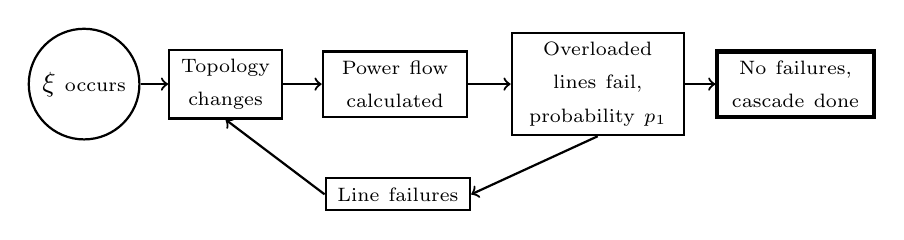
\begin{tikzpicture}
\draw [->,thick] (1,1) node[anchor=east, circle, draw]{$\xi$ \scriptsize occurs}
-- (1.35,1) node(TC)[anchor=west,text width=1.2cm,text centered,  rectangle, draw]{\scriptsize Topology changes};
\draw[->,thick] (TC)
--(3.3,1) node(PF)[anchor=west,text width=1.6cm,text centered, rectangle,draw]{\scriptsize Power flow calculated};
\draw[->,thick] (PF)
--(5.7,1) node(F)[anchor=west,text width=1.95cm, text centered, rectangle, draw]{\scriptsize Overloaded lines fail, probability $p_1$};
\draw[->,thick] (F)
--(8.3,1) node(DN)[anchor=west,text width=1.75cm, text centered,rectangle,draw,line width=1.5pt]{\scriptsize No failures, cascade done};
\draw[->,thick] (F.south)
--(5.2,-.4) node(LF)[anchor=east,text width=1.6cm, text centered, rectangle, draw]{\scriptsize Line failures };
\draw[->,thick] (LF.west)
-- (TC.south);

\end{tikzpicture} 
\caption{OPA simulation of a cascading power failure}
  \label{fig:cascade}
\end{figure}


The OPA model of the cascade process begins with an exogenous event, $\xi$, that effects the topology of the grid.  In their initial version, $\xi$ were the branches that randomly failed in an independent and identically distributed (I.I.D) manner, a Bernoulli trial with probability $p_0$.  Moments after the outage, the power flows are rerouted through the new topology based on the laws of physics.  In a longer time frame, it is possible for operators to take actions such as load shed and generator redispatch.  The resulting loading on the transmission lines is evaluated.  Their model then failed overloaded transmission lines with a Bernoulli trial with probability $p_1$ between  0.1 and 1.  After all overloaded lines are evaluated, a transition is made to the next stage.  Either there are no more outages, in which case the cascade is over, or more branch elements are outaged, the topology changes, and the operator is allowed to take recourse.  This process repeats until the system is stable and no outages occur.  Figure \ref{fig:cascade-example} shows a visual example of the cascading process.

For a given grid $\cG$ and initial demand $d_0$
\begin{description}\label{fast_opa}
\item[ Initial $ \xi $ ]  For $e=1,...,n_e$, draw $\omega$ from $U[0,1]$ and if $\omega \le p_0$, line $e$ is outaged.
\item[ ] \hspace{35px} \vdots 
\item[ Stage $m$ ]  Calculate the power flows $f_{m}$, a column containing the branch flows for all edges in $\cE$, by using DC power flow equations with demand vector $d_m$. 

For $e=1,...,n_e$, if branch flow $f_{em} \ge U_{em}$, draw $\omega$ from $U[0,1]]$ and if $\omega \le p_1$, outage line $e$.
\end{description}


%\documentclass{standalone}
%\begin{document}

\def \sc     { .65 }
\def \lw     { 1.25pt }

\begin{figure}
\centering
\begin{subfigure}[b]{.46\linewidth}
\begin{tikzpicture}[line width=\lw,scale=\sc]

\node[circle,fill=blue!20] (one) at (3,0) {\small 1};
\node[circle,fill=red!20] (two) at (5,0) {\small 2};
\node[rectangle,fill=green!20] (three) at (7,1) {\small 3};
\node[rectangle,fill=green!20] (four) at (5,1.75) {\small 4};
\node[rectangle,fill=green!20] (five) at (3,1.75) {\small 5};
\node[circle,fill=red!20] (six) at (2,3) {\small 6};
\node[rectangle,fill=green!20] (seven) at (5,3) {\small 7};
\node[circle,fill=red!20] (eight) at (3.85,3.45) {\small 8};
\node[rectangle,fill=green!20] (nine) at (7,3) {\small 9};
\node[rectangle,fill=green!20] (ten) at (5.85,4.1) {\small 10};
\node[rectangle,fill=green!20] (eleven) at (3.75,5) {\small 11};
\node[rectangle,fill=green!20] (twelve) at (2.35,5) {\small 12};
\node[rectangle,fill=green!20] (thirteen) at (.81,4.2) {\small 13};
\node[rectangle,fill=green!20] (fourteen) at (4,6) {\small 14};


\draw (one) -- (two) ;
\draw (one) -- (five);
\draw (two) -- (three) ; 
\draw (two) -- (four) ; 
\draw (two) -- (five) ; 
\draw (three) -- (four) ; 
\draw[red] (four) -- (five) ; 
\draw (four) -- (seven);
\draw (four) -- (nine);
\draw (five) -- (six) ; 
\draw (six) -- (eleven) ; 
\draw (six) -- (twelve) ; 
\draw (six) -- (thirteen) ; 
\draw (seven) -- (eight) ; 
\draw (seven) -- (nine) ; 
\draw (nine) -- (ten) ; 
\draw (nine) .. controls +(up:1.2cm) .. (fourteen) ;
\draw[red] (ten) -- (eleven); 
%\draw[red] (eleven) -- (twelve); 
\draw[red] (twelve) -- (thirteen);
\draw (thirteen) .. controls +(up:1.2cm) .. (fourteen) ; 
\end{tikzpicture}
\caption{Initial Event: The three red lines are outaged and the power flow redistributes.}
\end{subfigure}
\begin{subfigure}[b]{.46\linewidth}
\begin{tikzpicture}[line width=\lw,scale=\sc]

\node[circle,fill=blue!20] (one) at (3,0) {\small 1};
\node[circle,fill=red!20] (two) at (5,0) {\small 2};
\node[rectangle,fill=green!20] (three) at (7,1) {\small 3};
\node[rectangle,fill=green!20] (four) at (5,1.75) {\small 4};
\node[rectangle,fill=green!20] (five) at (3,1.75) {\small 5};
\node[circle,fill=red!20] (six) at (2,3) {\small 6};
\node[rectangle,fill=green!20] (seven) at (5,3) {\small 7};
\node[circle,fill=red!20] (eight) at (3.85,3.45) {\small 8};
\node[rectangle,fill=green!20] (nine) at (7,3) {\small 9};
\node[rectangle,fill=green!20] (ten) at (5.85,4.1) {\small 10};
\node[rectangle,fill=green!20] (eleven) at (3.75,5) {\small 11};
\node[rectangle,fill=green!20] (twelve) at (2.35,5) {\small 12};
\node[rectangle,fill=green!20] (thirteen) at (.81,4.2) {\small 13};
\node[rectangle,fill=green!20] (fourteen) at (4,6) {\small 14};

\draw[red] (one) -- (two) ;
\draw (one) -- (five);
\draw (two) -- (three) ; 
\draw[red] (two) -- (four) ; 
\draw (two) -- (five) ; 
\draw[red] (three) -- (four) ; 
%\draw (four) -- (five) ; 
\draw (four) -- (seven);
\draw (four) -- (nine);
\draw (five) -- (six) ; 
\draw (six) -- (eleven) ; 
\draw (six) -- (twelve) ; 
\draw (six) -- (thirteen) ; 
\draw (seven) -- (eight) ; 
\draw (seven) -- (nine) ; 
\draw (nine) -- (ten) ; 
\draw (nine) .. controls +(up:1.2cm) .. (fourteen) ;
%\draw (ten) -- (eleven); 
%\draw (twelve) -- (thirteen);
\draw (thirteen) .. controls +(up:1.2cm) .. (fourteen) ; 
\end{tikzpicture}
\caption{Stage 1: Lines 1-2, 2-4, and 3-4 are overloaded. Lines 1-2 and 3-4 fail, but line 2-4 remains in operation at an overloaded state. }

\end{subfigure}
\begin{subfigure}[b]{.46\linewidth}

\begin{tikzpicture}[line width=\lw,scale=\sc]

\node[circle,fill=blue!20] (one) at (3,0) {\small 1};
\node[circle,fill=red!20] (two) at (5,0) {\small 2};
\node[rectangle,fill=green!20] (three) at (7,1) {\small 3};
\node[rectangle,fill=green!20] (four) at (5,1.75) {\small 4};
\node[rectangle,fill=green!20] (five) at (3,1.75) {\small 5};
\node[circle,fill=red!20] (six) at (2,3) {\small 6};
\node[rectangle,fill=green!20] (seven) at (5,3) {\small 7};
\node[circle,fill=red!20] (eight) at (3.85,3.45) {\small 8};
\node[rectangle,fill=green!20] (nine) at (7,3) {\small 9};
\node[rectangle,fill=green!20] (ten) at (5.85,4.1) {\small 10};
\node[rectangle,fill=green!20] (eleven) at (3.75,5) {\small 11};
\node[rectangle,fill=green!20] (twelve) at (2.35,5) {\small 12};
\node[rectangle,fill=green!20] (thirteen) at (.81,4.2) {\small 13};
\node[rectangle,fill=green!20] (fourteen) at (4,6) {\small 14};

%\draw[red] (one) -- (two) ;
\draw (one) -- (five);
\draw (two) -- (three) ; 
\draw[red] (two) -- (four) ; 
\draw[red] (two) -- (five) ; 
%\draw[red] (three) -- (four) ; 
%\draw (four) -- (five) ; 
\draw (four) -- (seven);
\draw (four) -- (nine);
\draw (five) -- (six) ; 
\draw (six) -- (eleven) ; 
\draw (six) -- (twelve) ; 
\draw[red] (six) -- (thirteen) ; 
\draw (seven) -- (eight) ; 
\draw[red] (seven) -- (nine) ; 
\draw (nine) -- (ten) ; 
\draw (nine) .. controls +(up:1.2cm) .. (fourteen) ;
%\draw (ten) -- (eleven); 
%\draw (twelve) -- (thirteen);
\draw (thirteen) .. controls +(up:1.2cm) .. (fourteen) ; 
\end{tikzpicture}
\caption{Stage 2: On the new topology, lines 2-5, 6-13, and 7-9 become overloaded.  The cascade progresses by outaging lines 2-4 and 7-9.}
\end{subfigure}
\begin{subfigure}[b]{.46\linewidth}
\begin{tikzpicture}[line width=\lw,scale=\sc]


\node[circle,fill=blue!20] (one) at (3,0) {\small 1};
\node[circle,fill=red!20] (two) at (5,0) {\small 2};
\node[rectangle,fill=green!20] (three) at (7,1) {\small 3};
\node[rectangle,fill=green!20] (four) at (5,1.75) {\small 4};
\node[rectangle,fill=green!20] (five) at (3,1.75) {\small 5};
\node[circle,fill=red!20] (six) at (2,3) {\small 6};
\node[rectangle,fill=green!20] (seven) at (5,3) {\small 7};
\node[circle,fill=red!20] (eight) at (3.85,3.45) {\small 8};
\node[rectangle,fill=green!20] (nine) at (7,3) {\small 9};
\node[rectangle,fill=green!20] (ten) at (5.85,4.1) {\small 10};
\node[rectangle,fill=green!20] (eleven) at (3.75,5) {\small 11};
\node[rectangle,fill=green!20] (twelve) at (2.35,5) {\small 12};
\node[rectangle,fill=green!20] (thirteen) at (.81,4.2) {\small 13};
\node[rectangle,fill=green!20] (fourteen) at (4,6) {\small 14};

%\draw[red] (one) -- (two) ;
\draw (one) -- (five);
\draw (two) -- (three) ; 
%\draw[red] (two) -- (four) ; 
\draw[red] (two) -- (five) ; 
%\draw[red] (three) -- (four) ; 
%\draw (four) -- (five) ; 
\draw[red] (four) -- (seven);
\draw[red] (four) -- (nine);
\draw (five) -- (six) ; 
\draw (six) -- (eleven) ; 
\draw (six) -- (twelve) ; 
\draw[red] (six) -- (thirteen) ; 
\draw (seven) -- (eight) ; 
%\draw[red] (seven) -- (nine) ; 
\draw (nine) -- (ten) ; 
\draw (nine) .. controls +(up:1.2cm) .. (fourteen) ;
%\draw (ten) -- (eleven); 
%\draw (twelve) -- (thirteen);
\draw[red] (thirteen) .. controls +(up:1.2cm) .. (fourteen) ; 
\end{tikzpicture}
\caption{Stage 3: This has the effect of routing all power destined for load 8 through the north passage. Lines 13-14, 4-7, and 4-9 are outaged along the path. }
\end{subfigure}

\begin{subfigure}[b]{.46\linewidth}
\begin{tikzpicture}[line width=\lw,scale=\sc]


\node[circle,fill=blue!20] (one) at (3,0) {\small 1};
\node[circle,fill=red!20] (two) at (5,0) {\small 2};
\node[rectangle,fill=green!20] (three) at (7,1) {\small 3};
\node[rectangle,fill=green!20] (four) at (5,1.75) {\small 4};
\node[rectangle,fill=green!20] (five) at (3,1.75) {\small 5};
\node[circle,fill=red!20] (six) at (2,3) {\small 6};
\node[rectangle,fill=green!20] (seven) at (5,3) {\small 7};
\node[circle,fill=red!20] (eight) at (3.85,3.45) {\small 8};
\node[rectangle,fill=green!20] (nine) at (7,3) {\small 9};
\node[rectangle,fill=green!20] (ten) at (5.85,4.1) {\small 10};
\node[rectangle,fill=green!20] (eleven) at (3.75,5) {\small 11};
\node[rectangle,fill=green!20] (twelve) at (2.35,5) {\small 12};
\node[rectangle,fill=green!20] (thirteen) at (.81,4.2) {\small 13};
\node[rectangle,fill=green!20] (fourteen) at (4,6) {\small 14};


%\draw[red] (one) -- (two) ;
\draw (one) -- (five);
\draw (two) -- (three) ; 
%\draw[red] (two) -- (four) ; 
\draw[red] (two) -- (five) ; 
%\draw[red] (three) -- (four) ; 
%\draw (four) -- (five) ; 
%\draw (four) -- (seven);
%\draw (four) -- (nine);
\draw (five) -- (six) ; 
\draw (six) -- (eleven) ; 
\draw (six) -- (twelve) ; 
\draw (six) -- (thirteen) ; 
\draw (seven) -- (eight) ; 
%\draw[red] (seven) -- (nine) ; 
\draw (nine) -- (ten) ; 
\draw (nine) .. controls +(up:1.2cm) .. (fourteen) ;
%\draw (ten) -- (eleven); 
%\draw (twelve) -- (thirteen);
%\draw (thirteen) .. controls +(up:1.2cm) .. (fourteen) ; 
\end{tikzpicture}
\caption{Stage 4:  Finally, line 2-5 that is still overloaded is outaged. }
\end{subfigure}
\begin{subfigure}[b]{.46\linewidth}
\begin{tikzpicture}[line width=\lw,scale=\sc]


\node[circle,fill=blue!20] (one) at (3,0) {\small 1};
\node[circle,fill=red!20] (two) at (5,0) {\small 2};
\node[rectangle,fill=green!20] (three) at (7,1) {\small 3};
\node[rectangle,fill=green!20] (four) at (5,1.75) {\small 4};
\node[rectangle,fill=green!20] (five) at (3,1.75) {\small 5};
\node[circle,fill=red!20] (six) at (2,3) {\small 6};
\node[rectangle,fill=green!20] (seven) at (5,3) {\small 7};
\node[circle,fill=red!20] (eight) at (3.85,3.45) {\small 8};
\node[rectangle,fill=green!20] (nine) at (7,3) {\small 9};
\node[rectangle,fill=green!20] (ten) at (5.85,4.1) {\small 10};
\node[rectangle,fill=green!20] (eleven) at (3.75,5) {\small 11};
\node[rectangle,fill=green!20] (twelve) at (2.35,5) {\small 12};
\node[rectangle,fill=green!20] (thirteen) at (.81,4.2) {\small 13};
\node[rectangle,fill=green!20] (fourteen) at (4,6) {\small 14};


%\draw[red] (one) -- (two) ;
\draw (one) -- (five);
\draw (two) -- (three) ; 
%\draw (two) -- (four) ; 
%\draw[red] (two) -- (five) ; 
%\draw[red] (three) -- (four) ; 
%\draw (four) -- (five) ; 
%\draw (four) -- (seven);
%\draw (four) -- (nine);
\draw (five) -- (six) ; 
\draw (six) -- (eleven) ; 
\draw (six) -- (twelve) ; 
\draw (six) -- (thirteen) ; 
\draw (seven) -- (eight) ; 
%\draw[red] (seven) -- (nine) ; 
\draw (nine) -- (ten) ; 
\draw (nine) .. controls +(up:1.2cm) .. (fourteen) ;
%\draw (ten) -- (eleven); 
%\draw (twelve) -- (thirteen);
%\draw (thirteen) .. controls +(up:1.2cm) .. (fourteen) ; 
\end{tikzpicture}
\caption{Stage 5:  The system stabilizes into islands with generator 1 serving load 6.  However, loads 2 and 8 are out of service.}
\end{subfigure}
\caption[An example of the OPA cascading sequency]{ \label{fig:cascade-example} \small An example of a cascading power failure. Node 1 is a generator and nodes 2, 6, and 8 are loads.}
\end{figure}

%\end{document}


\subsubsection{Dynamic Equilibrium}

These opposing forces eventually find an equilibrium.  The equilibrium tends to be near critical points, which are points that have maximum power flow through the network for the nominal system capacity.  The system self-organizes toward these points, which maximize efficiency of its assets.  When the system approaches these critical points, the power flow becomes limited due to two possible causes:
\begin{itemize}
\item The power flows are limited due to transmission line constraints.  This type of critical point has larger blackouts, but happen less frequently.  In addition, the blackouts typically have  multiple lines tripping.
\item The power flows are limited due to generation capacity.  This results in frequent blackouts, but of smaller size.
\end{itemize}
However, it is also possible to be in an operating regime which is close to both types of critical points simultaneously.  When this is the case, blackouts of all sizes occur.  While this operating regime may not be good from a reliability standpoint, it has the desirable characteristic of being able to deliver the maximum power for the system.   That is, when these two points are balanced, the system is capable of maximum throughput from its generators to its loads with minimal excess capacity.  This is important from an economic perspective and a critical reason the system self-organizes to these types of points.  This type of point tends to be the cheapest way to supply all the loads with power, while statisfying the minimum system reliability standards.

\subsubsection{Additional Complexities}

The OPA model can be extended to include additional complexities for many different reasons.  It is always a balance of how much resources you have to solve the problem and the amount of resolution you need in the solution.  The base OPA model is easy and fast to replicate, however by trying to gain increased resolution in the output, the model becomes increasingly complex and difficult to solve in a timely manner.

In related work, Chen et. al. \cite{chen_2005} find many similar conclusions to the OPA model by using an extension which included a hidden failure model.  A hidden failure is undectable in normal operations, but as the system becomes disturbed, a relay may incorrectly trip.  These protective relays are in operation to protect the line from overloads and disconnect it from the system.  This work introduces a loading dependent failure model that trips neighboring lines to outaged components.  This hidden failure is exposed the first time a disturbance nearby occurs and if it doesn't fail then, it is assumed to be properly operating and future disturbances will not undergo this hidden failure mechanism.  The probability of these happening in the real world are non-negligble according to NERC data \cite{nerc_dawg}.  

This work displays many similar results to the OPA papers.  First, the power law behavior near critical loading can be seen by varying the system loading levels.  They find that by increasing spinning reserves the risk of big blackouts is greatly reduced.  The blackout size distribution tends toward an exponential distribution as reserve levels are increased.  By lowering the hidden failure rate, the system becomes more robust and larger blackouts become less likely.  Finally, they note that prompt control actions can reduce the risk of big disturbances.  While all of these results seem fairly straightforward, it points to the fact that the important aspects of the cascading process are being modeled and the effects are similar to what would happen in the real world.

Bienstock made several modifications \cite{bienstock_2011} to the original OPA model in order to remove some undesirable effects of the simulation, notably the erratic behavior of its output under small changes in the input.  To do this, he introduced the concept of memory to the system.  In order to see if a line is in or near an overloaded state, it uses a running time average of the current state and previous states.
\begin{equation}
\tilde{f}_{et} = \alpha f_{et} + (1-\alpha) \tilde{f}_{e\rho(t)}
\end{equation} 
Here, $f_{et}$ represents the power flow on edge $e$ at time $t$.  Then, $\tilde{f}_{et}$ is used in the overload and outage calculations.

In addition to including a memory, he also smoothed out the definition of an overloaded line by creating a step in between normal and overloaded states in which the failure probability was more than nominal but less than in the overloaded state.  Using $0 \le \epsilon \le 1$, for edge $e$, the following failure model smooths the effects of overloaded lines failing.
\begin{align}
\tilde{f}_{et} \ge (1+\epsilon) U_{et}			&	\hspace{10pt} \mbox{The line outages with certainty} 	\\
(1-\epsilon) U_{et} < \tilde{f}_{et} < (1+\epsilon) U_{et}	&	\hspace{10pt} \mbox{The line outages with probability }\frac{1}{2} 	\\
\tilde{f}_{et} \le (1-\epsilon) U_{et}			&	\hspace{10pt} \mbox{The line remains in operation} 
\end{align}

An AC power blackout model was developed at the University of Manchester (Manchester Model) by Nedic \cite{nedic_2006} and the original OPA authors.  This model is able to represent real world disturbances more accurately by using the full non-linear model that describes power flow.  This gives resolution into areas for generator instability, under-frequency load shedding, redispatch of active and reactive sources, and emergency load shedding.  The model has both automated control systems and operator recourse.  This model was used in OPA criticality works by Mei et. al. \cite{mei_2006}, including one with mechanisms using voltage stability margins \cite{mei_2008}.  However, the additional complexity comes at the cost of having to solve a nonlinear program and the loss of convergence gaurantees.  This is all done in order to represent something that is a companion to, but not the main driver of the cascading process (according to the Northeast outage working group, the main driver was angle instability not voltage instability).

Mei and others have worked to improve the accuracy of OPA by increasing the amount of details modeled \cite{mei_2009}.  In the fast dynamics, along with protective relays being modeled as hidden failures, they included a failure mechanism for the operational dispatch center that is responsible for generator redispatch.  In addition, they used a failure model where an underloaded line is failed with probability $p_1 \left( f_e/U_e \right)^N$, with $N=10$.  For the slow dynamics, they added a step that models a planning department by increasing the capacity of lines which have a loading rate $\left( f_{e}/ U_{e}  \right)$ greater than a set point.  

In 2013, Qi et. al. extended this model to include slow dynamics of vegetation growth and management as well as differential equations representing line heating.  Neglecting spatial variation and heating/cooling effects from   the environment, they model line temperature by a differential equation
\begin{equation}
\frac{dT(t)}{dt} = \alpha I^2 - \nu (T(t) - T_0)
\end{equation}
where $T(t)$ is the line temperature at $t$, $I$ current, $T_0$ initial temperature, and $\alpha$ and $\nu$ are calculated parameters.  This can be solved by assuming constant branch flow, $f$, to calculate the temperature over time
\begin{equation}
T(t) = e^{-\nu t}\left( T_0 - T_e(f) \right) + T_e(f)
\end{equation}
which can be used to find the final equilibrium temperature, $T_e(f)$ (a function of its constant power flow $f$ on the line), and time until a given temperature.  Using the calculated temperature, the horizontal span, and an elongation parameter, the line sag distance can be calculated.  When the minimum distance between lines and vegetation passes a breakpoint based on transmission line characteristics such as operational voltage, the line will be outaged.  They model the vegetation with a daily growth rate model and include a managment simulation in which they identify future potential hazards and cut down trees over time.  The statistical analysis of their model agreed well with historical data in China.


\subsection{Power Flow Review}
In order to run the OPA simulation of cascading failures, the ability to calculate power flows on the system is critical.  To model a balanced, three phase power flows, in full resolution we need to model complex power.  The alternating current of the power system can be represented by sine or cosine waves.  A three phase power system has three lines for each transmission element and each line has a wave that is out of phase with the other two.  Using one wave as a reference, the other phases will attempt to be 120 degrees behind reference and 120 degrees ahead of reference.  This improves the efficiency and quality of power for loads over a 2 line system as well as not requiring an excessive amount of lines for each transmission element.  

The details about complex power and electrical parameters of transmission elements to model balanced three phase power flow equations will be left to the appendix.\endnote{\textbf{Electrical Information}

Complex power has both real and reactive parts.  Alternating currents  on a circuit affect components of energy storage such as inductors (changing the current as opposed by a voltage)  or capacitors (store electrical charge).  Over one full cycle of the electricity changing direction, across any individual element there can be real power transferred.  However, there is also power which is stored and released within one cycle and the net energy transfer of this power is 0.  This is called reactive power and is modelled as the imaginary component of complex power.  Let $S_i$ be the complex power inject at some bus on the grid, that is
\begin{equation}
S_i = P_i + j Q_i = V_i I_i^*
\end{equation}
where $P$ is real power, $Q$ is reactive power, $V_i$ is complex voltage, and $I_i^*$ is the complex conjugate of current.  
	
To model a transmission line, the characteristic impedence is used.  At any point, there is complex current I, in each individual line in the transmission element.  Also, there is a complex voltage V difference between the lines.  The characteristic impedence (generalization of Ohm's Law) is then
\begin{equation} \label{impedence}
V/I = Z_0
\end{equation}

Here is a phasor representation of complex voltage $V_i = | V_i | e^{i (\omega t + \delta_i) }$, where the real voltage would be Re[$V_i$]$=\cos (\omega t + \delta_i)$.  Now, by modeling \ref{impedence} in phasor notation, we have 
\begin{equation}
 | V_i | e^{j (\omega t + \delta_V) } = | I_i | e^{j (\omega t + \delta_I) }  | Z_i | e^{j ( \delta_Z) } = |I||Z|e^{j (\omega t + \delta_I + \delta_Z)}
\end{equation}
For this equation to hold at all times $t$, we know that this must hold $\delta_V = \delta_I + \delta_Z$.  When an element has $\delta_Z = 0$, the current and voltage are exactly in phase and it is a purely resistive load with no reactive production or absorption. 

The lines can be modelled using a pi model (schematic diagram looks like $\pi$), which uses line parameters of resistance $R$, inductance $L$, conductance $G$, and capacitance $C$. 
\begin{equation}
Z_0 = \sqrt{  \frac{R+j \omega L}{G+j\omega C} }
\end{equation}
The system angular frequency is $\omega = 2 \pi f$, where $f$ is frequency here.  

If a transmission element is loaded at its surge impedence loading, it neither creates nor consumes reactive power.  This level is defined by 
\begin{equation}
SIL = V_{LL}^2 / Z_0
\end{equation}
Where $V_{LL}$ is the line to line voltage.  When a transmission line is at a level below this, it will supply reactive power and raise system voltages.  When the loading is above this level, the transmission line consumes reactive power, depressing voltages.
} \endnote{\textbf{Balanced Three Phase Power Flow}

In a balanced three phase system, at every vertex $i$, we have
\begin{equation}
S_i = P_i + j Q_i = V_i I_i^*
\end{equation}
In addition, with $KCL$, we have $I_i = \sum_{k=1}^n Y_{ik} V_k$, where $Y$ is the admittance bus matrix.  The admittance is the inverse of imdedence, that is
\begin{equation}
Y = G + j B = 1/Z = 1/(R + jX) 
\end{equation}
where $B$, the imaginary part of admittance, is susceptance and $X$, the imaginary part of impedence, is reactance.  Now we have that the complex power at every vertex $i$ is
\begin{equation}
S_i^* = P_i - j Q_i = V_i^* \sum_{k=1}^n Y_{ik} V_k
\end{equation}
By converting these into rectangular coordinates, we get two equations for each bus
\begin{align} \label{ac-pf}
P_i = \sum_{k=1}^n |V_i| |V_k| \left[ G_{ik} \cos (\delta_i - \delta_k) + B_{ik} \sin (\delta_i - \delta_k) \right]  \\
Q_i = \sum_{k=1}^n |V_i| |V_k| \left[ G_{ik} \sin (\delta_i - \delta_k) - B_{ik} \cos (\delta_i - \delta_k) \right]  
\end{align}

For each bus, in addition to $P_i$ and $Q_i$,  we have its voltage $|V_i|$ and its phase angle $\delta_i$.  So, we have $4 n_v$ variables and $2 n_v$ equations.  By supplying the value to $2 n_v$ variables and defining a slack bus, we can find unique values for the remaining $2n_v - 1 $ variables.  Depending on the type of bus, different variables are supplied.  If it is a generator, both $P$  and $V$ are supplied.  A load is defined by a $P$ and $Q$.  The slack bus is a generator in which the phase angle is set to 0.  The phase angle $\delta$ and reactive power production $Q$ are found for each generator and the phase angle $\delta$ and the voltage $|V|$ are found for the loads.}  These non-linear equations model the net power and reactive power injects as well as voltage and phase angle at each vertex of the power system.  A few simplifying assumptions will be made to allow the equations to become linear for the DC (decoupled) power flow equations.  Then, using the dc power flow model, basic economic dispatch and unit commitment models will be shown.  
%Finally, some pseudo-topological measures will be reviewed that will be useful in the optimization process.

\subsubsection{Decoupled Power Flow}
This model makes assumptions such as lossless lines, small voltage angle differences, and a flat voltage profile.  This is a common simplifying model which is used routinely in economic and reliability analysis of power systems.  A flat voltage profile implies that $\forall i \in \cV$, we have $V_i = 1$.  Small voltage angle difference in conjunction with sine and cosine give the following approximations
\begin{align}
\cos(\delta_i - \delta_j) &\approx 1	\\
\sin(\delta_i-\delta_j) & \approx \delta_i - \delta_j
\end{align}
In addition, since these lines are lossless, $R$ and $G$ are 0.  

The following equations represent the necessary constraints on the power flow in this lossless system.  The first equation represents the conservation of energy and the second equation represents Kirchoff's Current Law.  Conservation of energy implies that the sum of generation and demand is equal to 0 at every point in time.
\begin{align}	\displaystyle
\sum_{j | e=(i,j),  e \in \cE}{f_{e}} &= g_{i} -d_{i} \hspace{17px}   \forall i \in \cV   \label{pf1}
\\
\theta_{i} - \theta_{j} &= X_{e} f_{e}			\hspace{27px}	\forall e=(i,j) \mbox{ s.t. } e \in \cE   \label{pf2}
\end{align}
The value $p_{i} = g_{i} - d_{i}$ represents the net power inject for that node.  A reliability focused model would seek to maximize demand served at all points in time.

When a line is outaged, the power flow has obviously dropped to 0, that is $f_e = 0$.  In addition, the constraint \ref{pf2} to the system is no longer there and must be removed from the formulation.

\subsubsection{Economic Dispatch}
To clear the electricity market at a single point in time, a least cost dispatch model is used.  This model takes bids from generators, a known demand, as well as transmission and ramping constraints and finds a set of generator outputs which meet the demand at least cost.  Using a quadratic cost function for the generators (this cost function can be thought of as a bid from generators which includes the profit the generator would like to make for each marginal unit of production), the least cost dispatch model is as follows. 

The following model is a quadratic program with linear constraints.  The objective function is to minimize the cost of generation.  Typical least cost dispatch and unit commitment models will make various assumptions to allow for linear constraints versus the physical nonlinear constraints to which the power system is subject.  This is the most basic least cost dispatch model, which could be used for clearing the real-time market.  Models in use can have extensions such as ''$N-1$ constraints", which are reliability and security requirements.

\begin{subequations}
\begin{align}
 \min \sum_i \alpha_i g_i &+ \beta_i g_i^2	+ W_i(\tilde{d} - d_i)&	\\
g_i - d_i &= \sum_j f_{ij}	&	\forall i \in N 	\\
X_{ij} f_{ij} &= \delta_i - \delta_j & \forall (i,j) \in M \\
g_i  &\in \left[ g_i^- , g_i^+ \right]		&	\forall i \in N 	\\
f_{ij} &\in \left[ -U_{ij}, U_{ij} \right]	&	\forall (i,j) \in M 
\end{align}
\label{leastcostdispatch}
\end{subequations}

Here, $\alpha_i g_i + \beta_i g_i^2$ can be seen as the cost function for the generator at node $i$ and $W_i(\tilde{d} - d_i)$ is the cost for shedding load.  The generator is bounded between a maximum $g_i^+$ and minimum $g_i^-$ that represent its ramping rate over a specific time interval.  

The day-ahead market uses unit commitment models.  This model will have power flow equations for each $t \in \cT$.  These are integer programs due to the introduction of binary variables $y_{it}$, which take on the value 1 if the generator is switched on and 0 if the generator is off.  The following logical constraint enforces this by
\begin{equation}
y_{it} g_i^- \le g_{it} \le y_{it} g_i^+
\end{equation}
The cost function can then include a fixed cost for operating a generator, such as increased staff during operation.  This cost is not dependent on the level of production but rather if the plant is in an on or off state.  The cost function for each node $i$ and time period $t$ is
\begin{equation}
\alpha_i g_it + \beta_i g_{it}^2 + c_i y_{it}
\end{equation}
This subproblem will be used in a full day model in which the power flow problem is solved for each time period, while remaining feasible with respect to ramping rates and on and off times for generators.





\section{Multi-Stage Stochastic Programming}

We will use the framework of stochastic programming to model the dynamics of cascading power failure.  Each stage will represent an epoch at which one or more lines fail based upon their loading.  In order to do this, we will use a large mixed-integer linear program.

\subsection*{Mixed-Integer Program}
The mixed-integer formulation of cascading power failures uses binary variables to model line availability for stages in the cascade.  In addition to these extra variables, some input parameters are needed to formulate the problem.  First, the number of stages, $n_T$, for the cascade needs to be decided.  If large blackouts are of interest, this number should be large enough to not exclude the worst case scenarios.  Also, the number of outcomes at each node needs to be decided.  These outcomes represent the decision dependent uncertainty.  As the number of outcomes increases, the resolution of the uncertainty increases as well.  The size of the problem is related to the size of the stochastic tree, which is $n_o^{ n_T }$, where $n_o$ is the number of outcomes at each node.  As the subproblem is difficult, the computational complexity of this problem increases rapidly with the number of outcomes and stages.

\begin{figure}
\centering
\documentclass{standalone}
\usepackage{tikz}
\begin{document}
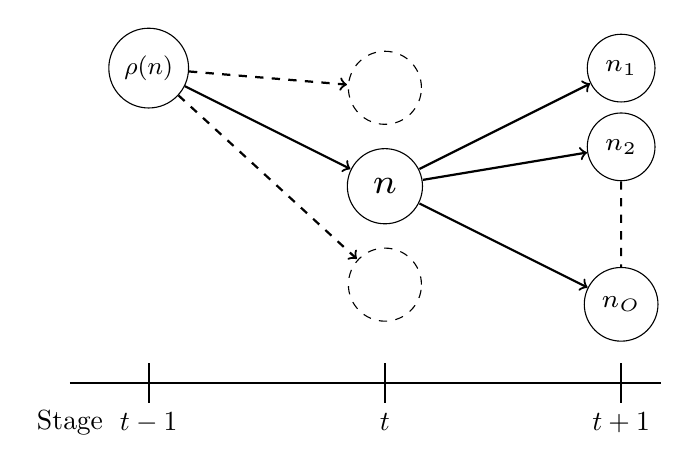
\begin{tikzpicture}

\draw (-1,2.5) node(RHO)[circle,draw]{\small $\rho(n)$ };
\draw (2,2.25) node(NUP)[circle,dashed,scale=2.8,draw]{ };
\draw (2,1) node(N)[circle,scale=1.8,draw]{\scriptsize $n$ };
\draw (2,-.25) node(NDOWN)[circle,dashed,scale=2.8,draw]{ };
\draw (5,2.5) node(N1)[circle,scale=1.3,draw]{\scriptsize $n_1$ };
\draw (5,1.5) node(N2)[circle,scale=1.3,draw]{\scriptsize $n_2$ };
\draw (5,-.5) node(NO)[circle,scale=1.3,draw]{\scriptsize $n_O$ };

\draw[thick,dashed, ->] (RHO) -- (NUP);
\draw[thick,->] (RHO) -- (N);
\draw[thick,dashed, ->] (RHO) -- (NDOWN);
\draw[thick,->] (N) -- (N1);
\draw[thick,->] (N) -- (N2);
\draw[thick,->] (N) -- (NO);
\draw[thick,dashed] (N2) -- (NO);

\draw[thick] (-2,-1.5) -- (5.5,-1.5);
\draw[thick] (-1, -1.75) -- (-1, -1.25);
\draw[thick] (2, -1.75) -- (2, -1.25);
\draw[thick] (5, -1.75) -- (5, -1.25);

\draw(-2,-2) node {Stage};
\draw(-1,-2) node {$t-1$};
\draw(2,-2) node {$t$};
\draw(5,-2) node {$t+1$};

\end{tikzpicture} 
\end{document}

\caption{Stochastic tree for Mixed-Integer Formulation}
  \label{fig:mip}
\end{figure}


\subsection{Decision Dependent Uncertainty}
In order to model the decision dependent uncertainty, a cumulative distribution function (cdf) for line failures based on loaded is needed.  This model uses a parameter, $R$, to represent the effective capacity of a line.  This is found by sampling from the cdf before formulating the problem.  This effective capacity represents the loading of the transmission line that will cause its failure.  This failure is represented in the binary variable, $z$. \\

In Mixed-Integer Programming, there have been standard equations developed to model logical conditions.  This problem has two logical conditions that need to be modeled in order to represent this decision dependent uncertainty.  First, the condition that the line will fail if it has more power flow than its effective capacity.
\begin{align*}
\mbox{If }
		\hspace{30px}&\left| f_{e\rho(n)} \right| > R_{en}  \\
\mbox{Then }
		\hspace{30px}&z_{en} = 0
\end{align*}

To model this logic, a Big-M constraint can be used, where M represents a large number.
\begin{align}
	f_{e\rho(n)} - R_{en} &\le M^R_e (1-z_{en})	\label{r1}\\
	f_{e\rho(n)} + R_{en} &\ge - M^R_e (1-z_{en})	\label{r2}
\end{align}
with $M^R_e = U_e - R_e$. \\

Now, when the line is available in stage $n$, that is $z_{en} = 1$, then the line flow in the predecessor node is within the effective capacity, -$R_{en} \le f_{e\rho(n)} \le R_{en}$.		\\

The second logical condition is that when the line is unavailable, the power flow on that branch is zero and the phase angles between the two nodes are not constrained. 
\begin{align*}
\mbox{If }
		\hspace{20px}&z_{en} = 0	\\
\mbox{Then }
		\hspace{20px}&f_{en} = 0  \hspace{10px} \mbox{ and}\\
				&\theta_{in} - \theta_{jn} - X_{e}f_{en} \mbox{ is arbitrary}
\end{align*}	

This can be achieved through the following equations.
\begin{align}
-U_{e} z_{en} \le f_{en} &\le U_{e} z_{en}	\label{lf1}\\
\theta_{in} - \theta_{jn} + X_e f_{en} &\ge -M^\theta_e(1-z_{en}) \label{lf2} \\
\theta_{in} - \theta_{jn} + X_e f_{en} &\le M^\theta_e(1-z_{en})  \label{lf3}
\end{align}
with $M^\theta_e = 2 \theta_{max} + X_e U_e$.


\subsection*{Failure Density Function}
The OPA simulation uses a step function for the failure probability of a line.  A line will fail if it $f_e \ge \alpha U_e$ with probability $p$.    To model that scenario here, a sample from the distribution can be used to form the effective capacity of the lines.  Let $\omega_n \equiv\left[ 0, 0, 1, 0, \cdots, 1\right]$  be a vector sampled from the probability distribution.  Now, a line will fail if $f_e \ge \alpha U_e$ and $w_{ne} =1$.  With this sampling, the effective capacity can be designed to incorporate this information.    
\begin{equation}
 R_{ne} = 
 \left\{ 
	\begin{array}{lr}
				\alpha U_e & \mbox{if } \omega_{ne}=1\\
			  U_e + \epsilon & \mbox{if } \omega_{ne}=0
	\end{array}
 \right. \label{r}
\end{equation}

The resulting set of effective capacities $R$ can be represented by a cumulative distribution function. The distribution in Figure \ref{cdf} is one example of a viable line failure distribution input.  It is the result of a uniform distribution for $\alpha$ between $L$ and 1 and Bernoulli trial with probability $p$ for $\omega$.  


\begin{figure}
\centering
\pgfplotsset{every axis plot/.append style={line width=2pt}}
\tikzset{
every pin/.style={fill=yellow!50!white,rectangle,rounded corners=3pt,font=\tiny},
small dot/.style={fill=black,circle,scale=0.3}
}

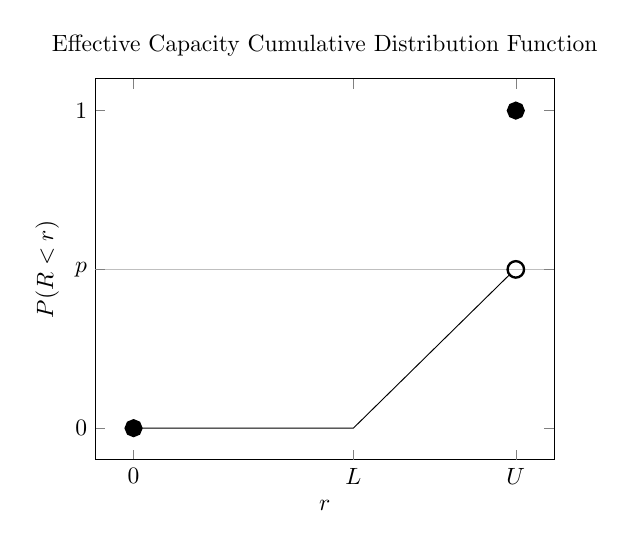
\begin{tikzpicture}[scale=.85]
\begin{axis}[ 
	xlabel=$r$,
	ylabel=$P( R < r )$,
	title = Effective Capacity Cumulative Distribution Function,
	unbounded coords = jump,
	xtick= {0},
	ytick= {0, 1},
	extra y ticks={.5},
	extra y tick style={grid=major},
	extra y tick labels={$p$},
	extra x ticks={.575,1},
	extra x tick labels={$L$, $U$},
scatter/classes={
 		 a={mark=o,line width=3.5pt},%
 		 b={mark=o,line width=1pt,scale=1.75}%
		}]
	\addplot[black] coordinates { 
		(0,0)		
		(.575,0)	
		(.985,.485) 		
		(1,inf)		
		(1,1)		
		};	
	\addplot[ 
		scatter,only marks,
		scatter src=explicit symbolic]
		coordinates {  
		(0,0)		[a]
		(1,.5)		[b]
		(1,1)		[a]
		};


	

\end{axis}
\end{tikzpicture}

\caption{ Example Effective Capacity Distribution for equation (\ref{r}) }
\label{cdf}
\end{figure}



\subsection{Feasible Cascades}
The cascading process begins with an intial exogenous event, $\xi \in \left\{ 0, 1 \right\}^{\magE}$.  The following equation enforces a line outage throughout the whole cascade for all $\xi = 1$.

\begin{equation}
z_{en} \le 1- \xi_e  \label{xi}
\end{equation}

Now, the set of all feasible cascades can be described as follows, 
\begin{equation}
\cX(\xi) \equiv \left\{ \left(d, p, f, z \right)  |  \mbox{ \cref{pf1,pf2,r1,r2,lf1,lf2,lf3,r,xi}  hold } \right\} 
\end{equation}
where $d = \left[ d_0, d_1, \cdots, d_N \right]$ is the set of vectors of demand served for each node in the scenario tree.  Now, this representation of the cascading process can be used in many ways.  One example is a chance constrained model, in which the operator requires a line to be available in a certain percentage of scenarios.  Another example is to use this as a subproblem in a larger planning model. 

\subsection{Least Cost Dispatch}
The following model is a least cost dispatch model that includes the effects from cascading failures due to a set of contingencies $\xi\in\Xi$.  
\begin{subequations}
\label{leastcost}
\begin{align} \displaystyle
	{\large \mbox{min}} \hspace{10px} &  \Expect_\Xi \sum_{in} \left[ C_{in}  p_{in,m}  + W_{in} (\hat{d}_{i} - d_{in,m}) \right]	\\
	&(d,p,f,z)_m  \in \cX(\xi_m)    \hspace{20px}   \forall \xi_m \in \Xi	
\end{align}
\end{subequations}
This can be adapted to several different problems in power systems.  The main difficulty with this multi stage stochastic program is computational complexity.  The program can be calibrated in order to produce similiar load shed distributions to the OPA model, however the number of outcomes and stages in the model needs to be small or the computational hurdle becomes too large.\endnote{\textbf{Model Calibration}

In order to get reliable output from the optimization routine, this model needs to be calibrated against the OPA simulation.  The primary calibration parameters are $L$ and $p$ in the line failure distribution as well as the costs for load shed, $W$, which depend upon the stage in the cascade.  The OPA simulation is a greedy algorithm, attempting to maximize demand served in the current stage without regard to the line failure consequences.  In order to capture this effect, more weight was placed on demand served in earlier stages of the cascade. \\

 The root problem used is comprised of 4 intitial outages and each outage has a scenario tree that is 4 stages long with 2 outcomes at each node.  The power system modeled is the IEEE 118 bus grid with a nominal demand of 3668 MW and around 29,600 MW in branch capacities.  The parameters chosen for the MSIP model were $p=.5$, $L =.575$.  The weight for the stages of the cascade were $[500, 10, .05, .0001]$, which seemed to capture the greedy behavior of the OPA simulation.  The OPA simulation used the step function failure model with $\alpha=.99$ and $p=.5$.  The output of the simulation and MSIP formulation are shown in Table (\ref{compare}) along with the load shed distribution for $\xi = [12,14,34,111]$ in Figure (\ref{dist}). 


% Calibrate ---------------------------------------------------------

\input{\mypathmsip/load_shed_distribution}


\input{\mypathmsip/comp_sim_msip}

%\input{line_outage}


}.


\section{Model Flexibility}
The primary strength of this formulation is the flexibility it has in using additional constraints and objectives to inform decision making about power systems.  All of these models can then be solved with commercial solver software without the need to develop additional specialized routines.  The first example is a chance constrained model, which enforces a probabilistic constraint on the number of line outages in any scenario. \endnote{\textbf{Chance Constraint on N-k Criteria}

In this model, constraints are used to express the probability that less than a given number of lines are outaged is close to 1.  A typical case in power systems would be that the system should not go beyond 1 contingency in a large percentage of scenarios.
\begin{equation}
P\left\{\text{Line Outage} \le k \right\} \ge 1 - \epsilon
\end{equation}
This can be done by adding another binary variable for each scenario that represents whether or not that scenario has less than $k$ outages.  Then these new binary variables will be summed and constrained by the given probability.
\begin{subequations}
\begin{align}
\sum_i z_{is} &\le	M_s \hat{z_s} + | \xi_s | + k \\
\sum_s \hat{z_s} &\le \epsilon | \cS |
\end{align}
\end{subequations}
where $M_s = | \cE | - | \xi_s | - k$.  The objective of this program would be to minimize load shed as in (\ref{leastcost}) such that the power system does not lose more than $k$ branches.
}  The second example is a redispatch model that moves to a generator configuration that is close to the original while minimizing the expected size of the cascade.\endnote{\textbf{Generator Redispatch}

This model tries to find an operating configuration that is within a given distance from the current operating regime and minimizes the worst case scenario outage.  The input for this model is the current operating configuration $(p_0, d_0)$ as well as a distance vector $\delta$ that represents how far each generator can move from its current output levels.  In this case, the root node of the stochastic tree will have variables that represent initial generator output levels and the child trees will be constrained from how far they can move from this.  Also, a continuous variable will be added that represents the amount of load shed in the worst case scenario.  The objective will be to minimize this worst case scenario.  
\begin{equation}
p - p_0 \le \delta
\end{equation}
\begin{equation}
l \ge \sum_i \hat{d}_i - d_{is}
\end{equation}
aim to min 
This program could be used when the system is becoming close to unstable and cost concerns become less of a priority than system stability.
}  Another exampe is a reserve planning model that allocates reserves among the generators in such a way as to minimize the worst case failure.\endnote{\textbf{Operating Reserves}

In this case an operating configuration need not be given.  The program can either search for an operating configuration as well as reserves or given an operating configuration, allocate the reserves.  These operating reserves determine where the system is able to relieve congestion in a contingency.
\begin{align}
p_{in} + r_{in} &\le \overline{P}_i \\
p_{in} &\le p_{i\rho (n)} + r_{i\rho (n)} \\
\sum_i r_{in} &\le \beta \sum_i \hat{d}_i 
\end{align}
where $\beta$ is the level of operating reserves alotted for the system.
}  Finally, the example we will use is a transmission expansion model that allocates a budget for capacity expansion on the grid in such a way as to minimize the expected size of the cascade.  This will have computation results and compare them with the OPA simulation to a simple heuristic which allocates the expansion budget.




\subsection{Transmission Expansion}
Using the MIP formulation, a stochastic program can be developed to model planning decisions with respect to cascading power failures.  Consider the problem of transmission expansion.  A set of contingencies, $\xi \in \Xi$, has been identified as the primary risk for initiating a cascading event.  There is a budget to use for expansion and the objective is to allocate the budget in such a way as to minimze some risk measure of load shed for the cascading power failures. \\

Let $x$ be the design variable, which is decided at the root node and represents additional capacity on power lines.  This affects the constraint set such that equations (\ref{lf1}) and (\ref{r}) become  
\begin{align}
-(U_{e}+x_e) z_{en} \le f_{en} \le (U_{e}+x_e) z_{en} &	\label{lfm}	\\
 R_{ne} = 
 \left\{ 
	\begin{array}{lr}
				\alpha (U_e + x_e) & \mbox{if } \omega_{ne}=1\\
			  (U_e + x_e) + \epsilon & \mbox{if } \omega_{ne}=0
	\end{array}
 \right. \label{rm}
\end{align}



\begin{figure}
\centering
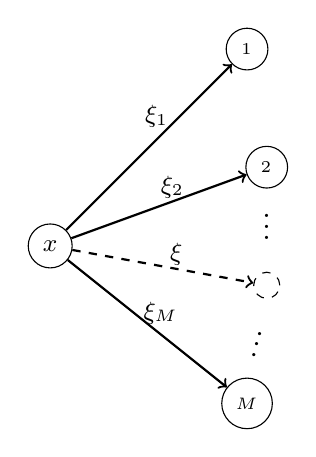
\begin{tikzpicture}

\draw (.5,.5) node(ROOT)[circle,draw]{\small $x$ };
\draw (3,3) node(ONE)[circle,draw]{ \small $\cX_1$ };
\draw (3.25,1.5) node(TWO)[circle,draw]{ \small $\cX_2$ };
\draw (3.25,.85) node(DOTONE){ \large $\vdots$ };
\draw (3.25,0) node(N)[circle,dashed,draw]{ \small $\cX$ };
\draw (3.15,-.65) node(DOTTWO)[rotate=-15]{ \large $\vdots$ };
\draw (3,-1.5) node(S)[circle,draw]{ \small $\cX_M$ };

\draw (1.85,2.15) node(OMG1){ \small $\xi_1$ };
\draw (2.05,1.25) node(OMG2){ \small $\xi_2$ };
\draw (2.1,.4) node(OMG){ \small $\xi$ };
\draw (1.9,-.35) node(OMGS){ \small $\xi_M$ };

\draw[thick, ->] (ROOT) -- (ONE) ;
\draw[thick,->] (ROOT) -- (TWO);
\draw[thick,dashed, ->] (ROOT) -- (N);
\draw[thick,->] (ROOT) -- (S);

%\draw[thick,dashed] (TWO) -- (N);
%\draw[thick,dashed] (N) -- (S);

\end{tikzpicture} 
\caption{Scenario Tree for Two Stage Problem}
  \label{fig:mip}
\end{figure}



The objective is to allocate a budget for capacity additions in order to reduce the expected blackout size.  $W_{in}$ is the cost of load shed at bus $i$ in node $n$ of the scenario tree.  $B$ is the budget for capacity expansion.
\begin{subequations}

\begin{align} \displaystyle
	{\large \mbox{min}} \hspace{10px} &  \Expect_\Xi \sum_{in} \left[ C_{in}  p_{in,m}  + W_{in} (\hat{d}_{i} - d_{in,m}) \right]	\\
	&(d,p,f,z)_m  \in \cX(\xi_m)    \hspace{20px}   \forall \xi_m \in \Xi	\\
	& \underline{X}_e y_e \le x_e \le \overline{X}_e y_e \hspace{35px} \forall e \in \cE\\
	&\sum_e x_e \le B_x 	\\
	& \sum_e y_e \le B_y  
\end{align}
\label{TX}
\end{subequations}



\subsection{Computational Implementation}
The model outlined in (\ref{TX}) is solved using Gurobi 4.5.  The stopping criteria was either a 40\% optimality gap or 10,000s.  The program was run for several different expansion budgets, with both the total budget and the maximum number of lines being changed.  The output of this model is a vector $x$ which represents the amount of capacity to add to each power line on the grid.  This is used to modify the initial grid and run the OPA simulation to find the effects it has on the system.  In order to find out whether these solutions are reasonable or not, a heuristic was developed to compare against.

The heuristic used is based on a large number of OPA simulation runs in which the power lines were ranked in descending order based on the percentage of runs in which that given power line was outaged.  Then, for a given total budget $B_x$ and maximum number of changed lines $B_y$, the heuristic picks the top $B_y$ lines in the list and then distributes the budget $B_x$ evenly over the lines.  The OPA simulation is used to compare the results of the two models.  Since the MSIP was calibrated based on the 4 contingencies, a second set of 4 random initial contingencies to start the OPA process to evaluate the effects.




\begin{figure}
 \centering
	\begin{tikzpicture}
		\begin{axis}[xlabel=$LS$ (MW), ylabel=$P($Load Shed $> LS )$
				,legend pos=north east
				,grid=major,
				,xmin=-25,xmax=1300
				,title=\mbox{Load Shed Distribution} ]


 	\addplot[red,line width=2pt] table[x=ls, y=prob] {./data/d25k20.dat};
	\addlegendentry{design}
	
	\addplot[blue,line width=2pt] table[x=ls, y=prob,mark=square] {./data/dumb25k20.dat};
	\addlegendentry{heuristic}

	\addplot[black,line width=2pt] table[x=ls, y=prob,mark=square] {./data/sim.dat};
	\addlegendentry{nom}




		\end{axis}	
	\end{tikzpicture}
  \caption{Load Shed Distribution for the OPA simulation and MSIP formulation}
 \label{dist}
\end{figure}

% Calibrate ---------------------------------------------------------

\section{Results and Conclusion}
After several trials, we found this solution methodology to be inadequate.  Due to the computational difficulty, the stochastic tree could only have around 4 stages with 3 outcomes per node in ideal settings by trial and error.  When using 4 initial contingencies, only sometimes were solutions found within a 40\% optimality gap.  This course representation of the underlying uncertainty made it a poor representation of the effects of the decision variables on the OPA simulation.  However, this approach may be successful if more analysis could determine highly probable failure sequences which need to be protected against.

Using the OPA simulation as a reference for how the grid may respond to cascading power failures, a mixed integer model was developed which represents the cascading effects over a fixed number of outcomes and stages.  While this model can be difficult computationally due to the decision dependent uncertainty, it is extremely flexible.  The model can be used to include cascading effects in a wide range of power system problems with optimality criteria ranging from least cost to minimize worst case problems.  A computation example was done on transmission expansion, which showed the model was able to better than a reasonable heuristic, even though it was only solved to a 40\% optimality gap.  Future work can be done in order to improve the solve time for these types of models based on techniques developed in stochastic and mixed integer optimization.

%\theendnotes
%\setcounter{endnote}{0}

\newcommand{\mypathdfo}{../thesis/dfo}
\newcommand{\mypathdfodata}{../thesis/dfo/data}
\newcommand{\scd}{\cD_\oplus}
\newcommand{\btu}{\bigtriangleup}
\chapter{Solving Design Problems}

The cascading model built in chapter \ref{msip-model} is too hard to optimize at the scale we need to model the uncertainty in the cascading process.  In order to work around this difficulty, we will decompose the multi-stage structure of this problem and simulate the entire cascading process.  The primary benefit is removing the temporal linked binary variables for line outages from the master problem allowing sequential evaluation of the decision dependent uncertainty.  This lets us parallelize the OPA evaluations to increase the computational effort.

In order to optimize design problems using the OPA simulation for risk metrics, we need to first understand the characteristics of the cascading process and the effects that generation, reserves, and line limits have on the resulting load shed distributions.  Then, we can modify existing derivative free frameworks to optimize this simulation and utilize exploratory steps to improve local performance and global strategies to find near optimal decisions.

The OPA simulation provides fundamental difficulties to the optimization process.  The function evaluations are non convex nor continuously differentiable.  It is inherently noisy and the load shed distribution is wide, often characterized by its power law distribution.  Some of these effects can be smoothed away by employing a wide range of potential initiating events, however it may be important to optimize against a small subset of events that have a higher likihood of occurence and are known to be risky.  In this case, the non convexity and discontinuity are most apparent.

To begin, an overview of derivative free optimization will be given.  A general class of direct search algorithms will be explored for its convergence properties as well as flexibility.  Model based methods, as well as accessory information, can be used to speed up the standard direct search methods.  Then, initial experimentation on the OPA model will be given as well as the implementation and variance reduction strategies.  A modified algorithm will be developed and compared against vanilla algorithms of DFO to show the benefit of accessory information. 

\section{Literature Review}
This section will give an overview to the history and current state of derivative free optimization.  The foundation for direct search and model based search of DFO techniques will be explored to be used in solution methods for the OPA optimization procedure.  The DFO field has been around for some time now and has seen a resurgence over the last decade and a half with the only textbook at less than 5 years old (Conn, Scheinberg, Vicente) \cite{conn_2009}.  Kolda et. al. provide an extensive work on direct search methods and its extensions in \cite{kolda_2003}. 
\subsection{Derivative Free Optimization}
This class of optimization strategies covers a wide-range of problems and techniques.  In general, the problem has a function $f: \R{n} \rightarrow \R{}$ that takes a decision variable $x \in \R{n}$ and returns a scalar. 
\begin{equation}
\min_{x \in \R{n}} f(x)
\end{equation}
The primary problem attribute that makes DFO a good choice for solution method is that standard gradient or Newton based method will not work.  This can be due to a variety of reasons, a common one being simulation-based optimization.  Here, the derivative is unavailable symbolically (through hard work or automatic differentiation schemes) and, perhaps due to stochastic or numerical noise, is unable to be calculated with finite difference methods.  Even if the underlying function is smooth, a costly function evaluation may make the finite difference approach undesirable due to the considerable time to calculate full gradients.

While still useful for smooth functions with a Lipschitz continuous derivatives, these methods can shine in nonsmooth and even non-convex application.  Direct search methods work by searching in many directions in order to guarantee a descent direction is chosen.  This has the ability to provide robustness against noise that may mislead gradient based methods using a single search direction.  In addition, by using relatively large step size the trial points provide a smoothing affect to the function which allow it to ignore high-frequency noise until it is close to a lower-frequency, higher amplitude minimum.  Contrary to problem application, we will assume a smooth function with a Lipschitz continuous derivative in order to find convergence results for different algorithms.  No guarantees can be made for the nonsmooth problems, however in practice these techniques are relatively successful for this class of problems

\subsubsection*{History}
\begin{figure}
\centering
\begin{tikzpicture}[
  level 1/.style={sibling distance=40mm},
  edge from parent/.style={->,draw},
  >=latex]


% root of the the initial tree, level 1
\node[root] (root) {\large \textbf{ Derivative Free Optimization}}
% The first level, as children of the initial tree
  child {node[level 2] (c1) {Direct Search}}
  child {node[level 2] (c2) {Model Based}}
  child {node[level 2] (c3) {Heuristics}}
  child {node[level 2] (c4) {Global}};

\node[oracle] (fo) at (5.1,2.1){Function Oracle};
\node[level 2 oracle,below of = fo,xshift=5pt] (o1) {Dimension Reduction};
\node[level 2 oracle,below of = fo,xshift=80pt, yshift=-20pt] (o2) {Variance Reduction};
\node[level 2 oracle,below of = o1,yshift=-10pt] (o3) {Accessory Information};
  \draw[->] (fo.190) |- (o1.west);
  \draw[->] (fo.190) |- (o2.west);
  \draw[->] (fo.190) |- (o3.west);

\draw[<->,very thick,dashed] (root) -- (fo.west);

% The second level, relatively positioned nodes
\begin{scope}[every node/.style={level 3}]
%\node [below of = c1, xshift=15pt,yshift=-5pt] (c11) {Generalized Pattern Search};
\node [below of = c1,xshift=15pt,yshift=-5pt] (c11) {Generating Set Search}; %with bound constraints
\node [below of = c11,yshift=0pt] (c12) {Mesh Adaptive};
\node [below of = c12] (c13) {Geometric, Simplex};

\node [below of = c2, xshift=15pt,yshift=2pt] (c21) {Trust Regions};
\node [below of = c21] (c22) {Implicit \newline Filtering};
\node [below of = c22,yshift=-5pt] (c23) {Stochastic \newline Approximation};

\node [below of = c3,xshift=15pt,yshift=2pt] (c31) {Particle Swarm};
\node [below of = c31] (c32) {Simulated \newline Annealing};
\node [below of = c32,yshift=-5pt] (c33) {Genetic \newline Algorithms};

\node [below of = c4, xshift=15pt,yshift=-5pt] (c41) {Nested \newline Partitioning};
\node [below of = c41, yshift=-2pt] (c42) {Space Filling};
\node [below of = c42,yshift=7pt ] (c43) {Global Model}; %Response Surface, radial basis functions, kriging
\end{scope}

% lines from each level 1 node to every one of its ``children''
\foreach \value in {1,2,3}
  \draw[->] (c1.195) |- (c1\value.west);

\foreach \value in {1,...,3}
  \draw[->] (c2.195) |- (c2\value.west);

\foreach \value in {1,...,3}
  \draw[->] (c3.195) |- (c3\value.west);

\foreach \value in {1,...,3}
  \draw[->] (c4.195) |- (c4\value.west);
\end{tikzpicture}

\caption{DFO methods for continuous variable optimization}
\end{figure}
Derivative-free techniques for optimizing problems have literature dating back to the 60's when Hookes and Jeeves \cite{hooke_1961} proposed a simple search method to find a maximum or minimum when classical methods were unfeasible.  Since then, direct search methods have seen many improvements both to their performance in practice and results in theory.  Modern direct search methods are able to conform to local topology as well as guarantee convergence to stationary points.  New methods are beginning to use probabilistic search procedures to improve in performance as well as increase the classes of problems they are able to solve.

Geometry based methods also started in the 60's with Nelder and Mead \cite{nelder_1965} using the geometric simplex and operations such as reflection, expansion, and contraction.  These methods can be useful as they naturally conform to local topology, however the geometry can often degenerate and converge to a non-optimal point.  Modern methods can use safeguarding techniques to prevent this or restart a simplex when it has deteriorated.  

Heuristic search procedures showed up in the 70's and have continued to be used throughout with many papers in practical application.  Common procedures such as genetic algorithms (1975) \cite{holland_1975}, simulated annealing (1983) \cite{kirkpatrick_1983}, and particle swarm (1995) \cite{eberhart_1995} \cite{kennedy_1995} are used throughout engineering and physic disciplines, partly due to their ease in application and decent practical performance.  While good for practical applications, they lack the more rigorous theory for convergence that is behind direct search and model based methods.

Model-based methods are very good at using function evaluations and spend considerably more effort to choose new points.  These interpolation based strategies were around at least by 1973 \cite{winfield_1973} and assume the model is accurate within its trust-region.  The method procedes by minimizing its model and using that as a new trial point.  Modern implementations can use linear models \cite{powell_1994}, quadratic models \cite{powell_2002}, or perhaps a good compromise being underdetermined quadratic models.

Finally, global based strategies are used in conjunction with many of the previous models in order to work toward global optima. One primary avenue is partitioning models.  These partions have trial points at the extreme points of the partion (1972)\cite{shubert_1972}, the center point (1993) \cite{jones_1993}, or arbitrary points within (1999) \cite{huyer_1999} and typically work by building underestimators of the function using the Lipschitz constant or an estimate.  Another strategy employed is surrogate functions to opitimize instead of the original function.  Common versions are response surfaces, kriging, and radial basis functions.  

A more complete history and overview of current derivative free methods as well as numerical tests for a large, diverse set of solvers can be found in \cite{rios_2013}.  Now we turn to direct search and model based methods to understand their implementation, performance, and convergence properties.


\subsubsection*{Gradient Line Search}
To start, a quick overview of line search methods and properties to guarantee convergence will be given.  These properties will be used as a comparison for comparable properties used in DFO methods.  Line search methods move in a descent direction and have constraints on step length in order to ensure convergence.  Assuming our function is continuously differentiable and letting $\alpha$ be a step size and $d$ a direction, we have
\begin{equation}
f(x + \alpha d ) = f(x) + \alpha \grad f(x) d  + o (\alpha)
\end{equation}
and by setting $d = -\grad f(x)$ we are guarenteed to reduce $f$ for sufficiently small step sizes $\alpha$.  We can see that any direction that is sufficiently in line with the negative gradient of $f$ will lead to a decrease, that is
\begin{equation}
-\grad f(x_k)^T d_k > 0
\end{equation}
Additionally, a near orthogonal direction to the gradient will lead to poor progress in search and convergence.  The angle between the search direction and the negative gradient needs to be bounded away from 0.  In the typical line search, this angle condition is
\begin{equation}
\frac{-\grad f(x_k)^T d_k}{\norm{\grad f(x_k) } \norm{d_k}} \geq c > 0
\end{equation}
and is automatically satisfied for $d_k = -\grad f(x_k)$.

A simple decrease condition $f(x_{k+1}) < f(x_{k})$ is not enough to guarantee convergence, due to the existence of sequences of points moving in a descent direction with a limit point other than the minimum.  This is related to the step size and both too short and too long of step sizes can cause problems.  The Armijo-Goldstein-Wolfe conditions prevent these problems by constraining the step length 
\begin{align}
f(x_k + \alpha_k d_k) \le f(x_k) + c_1 \alpha_k \grad f(x_k)^T d_k  \label{step_length_1}\\
\grad f (x_k + \alpha_k d_k)^T d_k \ge c_2 \grad f(x_k)^T d_k \label{step_length_2}
\end{align}
with $0 < c_1 < c_2 < 1$.  Typically, one needs to only enforce too long of steps (eq. \ref{step_length_2}) since there are no too short of steps (eq. \ref{step_length_1}) due to backtracking schemes.


\subsection{Direct Search}
An overview of the convergence results for a standard direct search method will be given. Positive spanning sets as well as the cosine measure are used to bound the angle between the polling directions and the negative gradient.  Then, using the subsequence of unsuccessful iterates, the trial steps become arbitrarily small and $x$ will approach a limit point.  We will need the assumption that the gradient is Lipschitz continuous with constant $M$
\begin{equation}
\norm{\grad f(y) - \grad f(x)}  \leq M \norm{ y - x }
\end{equation}

\begin{figure}
\centering
\begin{tabular}{c c}
\begin{tikzpicture}[ 
   scale=5,
    axis/.style={very thick, ->, >=stealth'},
    important line/.style={thick, color=red, ->},
    dashed line/.style={dashed, thin},
    pile/.style={thick, ->, >=stealth', shorten <=2pt, shorten
    >=2pt},
    every node/.style={color=black}
    ]
    % axis
    \draw[axis] (-0.1,0)  -- (1.1,0) node(xline)[right]
        {$x_1$};
    \draw[axis] (0,-0.1) -- (0,1.1) node(yline)[above] {$x_2$};
    % Lines
    \draw[pile] (.5,.5) coordinate (x) -- (.775,.5)
        coordinate (d2) node[right, text width=5em] {$d_2$};
    \draw[pile] (.5,.5) coordinate (x) -- (.3,.3)
        coordinate (d1) node[right, text width=5em] {$d_3$};
    \draw[pile] (.5,.5) coordinate (x) -- (.3,.7)
        coordinate (d3) node[right, text width=5em] {$d_1$};
    \fill[red]  (x) +(0,0) coordinate (.5,.5) circle (.4pt)
        node[above] {$x$};

    \draw[important line] (.5,.5) coordinate (x) -- (.78,.925)
        coordinate (gf) node[right, text width=5em] {$-\grad f(x)$};

     \draw[dashed line] (d2) -- (.78,.5);
     \draw[dashed line] (gf) -- (.78,.5);

     \path[clip] (.5,.5) -- (.78,.5) -- (.78,.925);

     \node[circle,draw=blue,minimum size=25pt] at (.5,.5) (circ) {};
     \node at(.62,.55) {$\theta$};


\end{tikzpicture}
&
\begin{tikzpicture}[ 
   scale=5,
    axis/.style={very thick, ->, >=stealth'},
    important line/.style={thick, color=red, ->},
    dashed line/.style={dashed, thin},
    pile/.style={thick, ->, >=stealth', shorten <=2pt, shorten
    >=2pt},
    every node/.style={color=black}
    ]
    % axis
    \draw[axis] (-0.1,0)  -- (1.1,0) node(xline)[right]
        {$x_1$};
    \draw[axis] (0,-0.1) -- (0,1.1) node(yline)[above] {$x_2$};
    % Lines
    \draw[pile] (.5,.5) coordinate (x) -- (.75,.5)
        coordinate (d2) node[right, text width=5em] {$d_2$};
    \draw[pile] (.5,.5) coordinate (x) -- (.5,.25)
        coordinate (d3) node[right, text width=5em] {$d_3$};
    \draw[pile] (.5,.5) coordinate (x) -- (.5,.75)
        coordinate (d1) node[ text width=3em] {$d_1$};
    \draw[pile] (.5,.5) coordinate (x) -- (.25,.5)
        coordinate (d4) node[above right, text width=5em] {$d_4$};
    \fill[red]  (x) +(0,0) coordinate (.5,.5) circle (.4pt)
        node[above left] {$x$};

    \draw[important line] (.5,.5) coordinate (x) -- (.78,.925)
        coordinate (gf) node[right, text width=5em] {$-\grad f(x)$};

     \draw[dashed line] (d1) -- (.5,.925);
     \draw[dashed line] (gf) -- (.5,.925);

     \path[clip] (.5,.5) -- (.78,.925) -- (.5,.925);

     \node[circle,draw=blue,minimum size=25pt] at (.5,.5) (circ) {};
     \node at(.535,.625) {$\theta$};
\end{tikzpicture}
\\
$N+1$ points & $2N$ points 
\end{tabular}
%    \draw[important line] (.15,.85) coordinate (C) -- (.85,.15)
%        coordinate (D) node[right, text width=5em] {$\mathit{NX}=x$};
    % Intersection of lines
 %   \fill[red] (intersection cs:
%       first line={(A) -- (B)},
%       second line={(C) -- (D)}) coordinate (E) circle (.4pt)
%       node[above,] {$A$};
    % The E point is placed more or less randomly
%    \fill[red]  (E) +(-.075cm,-.2cm) coordinate (out) circle (.4pt)
%        node[below left] {$B$};
    % Line connecting out and ext balances
%    \draw [pile] (out) -- (intersection of A--B and out--[shift={(0:1pt)}]out)
%        coordinate (extbal);
%    \fill[red] (extbal) circle (.4pt) node[above] {$C$};
    % line connecting  out and int balances
%    \draw [pile] (out) -- (intersection of C--D and out--[shift={(0:1pt)}]out)
%        coordinate (intbal);
%    \fill[red] (intbal) circle (.4pt) node[above] {$D$};
%    % line between out og all balanced out :)
 %   \draw[pile] (out) -- (E);

\caption{Positive spanning sets for $\R{2}$}
\end{figure}

A positively spanning set $\cG$ of $\R{n}$ can write any vector $v \in \R{n}$ as a positive combination of points $d_i \in \cG$,  $\beta_i \geq 0 \forall i$
\begin{equation}
v = \sum_i \beta_i d_i
\end{equation}
Kolda, Lewis, and Torczon \cite{kolda_2003} call this a generating set of $\R{n}$ which makes the foundation for their class of generating set search methods.  This is a large class of problems which generalize lattice methods of Berman \cite{berman_1966} \cite{berman_1969} as well as their own older methods \cite{torczon_1997} \cite{lewis_2000} and include the original Hookes and Jeeves method\cite{hooke_1961}.  Generating sets can be adapted for explicit linear constraints to conform to local topology.\endnote{\textbf{Explicit Linear Constraints}

These constraints can be dealt with in the framework of generating set search.  Here, one needs to concern themselves only with the nearby active constraints and a satisifactory set of polling directions would be a positive spanning set of the tangent cone of the nearby active constraints. 
\begin{figure}
\centering
\input{\mypathdfo/fig-genset}
\caption{Generating set for polar cone to conform to local topology}
\end{figure}
The compass search for standard bound constraints conforms to the constraints ideally and no modifications need to be made other than letting $f = \inf $ for $x$ out of bounds and not waste the time on the function evaluation.
}

By searching in all directions of a generating set of $\R{n}$, we are guaranteed to have a direction which is somewhat aligned with the descent direction $f$, if it is smooth and has a Lipschitz continous derivative.  To make this matter concrete, the cosine measure of a set is the worst case scenario for the descent direction aligning with any direction of the generating set $\cG$.
\begin{equation}\label{kappa}
\kappa ( \cG) \equiv \min_{v \in \R{n}} \max_{d \in \cG} \frac{v^t d}{\norm{v} \norm{d}}
\end{equation}
This can be calculated for various generating sets, for example the compass search generating set gives $\kappa(\scd) = \frac{1}{\sqrt{n}}$ where $n$ is the dimension of the problem.  This begins to show why this method will struggle as the dimension of the problem increases.  The cosine measure of the search directions must be bounded below to ensure the search directions do not deteriorate.

\begin{algorithm}
\caption{Compass search, a generating set search}\label{dfo_genset}
\begin{algorithmic}
\Procedure{CS}{$f:\R{n} \rightarrow \R{}$}
\State $x_0 \in \R{n}$ Initial guess
\State $\bigtriangleup_{tol} >0$ Termination criteria
\State $\bigtriangleup_0 > \bigtriangleup_{tol} >0$ Initial neighborhood
\BState For each $k=1,2,...$

\State Let $\scd =\left\{ \pm e_i| i=1,...,n\right\}$ be the set of coordinate directions
\If{ $\exists d_k \in \scd$ such that $f(x_k + \btu_k d_k ) < f(x_k)$}
\State $x_{k+1} \gets x_k + \btu_k d_x$
\State $\btu_{k+1} = \btu_k$
\Else
\State $x_{k+1} \gets x_k$
\State $\btu_{k+1} = \frac{1}{2} \btu_k$
\If{$\btu_{k+1} < \btu_{tol}$} terminate \EndIf
\EndIf
\EndProcedure
\end{algorithmic}
\end{algorithm}

The key to convergence comes during the unsucessful steps.  The typical analysis will show that the gradient can be bounded at unsucessful steps by the step size and that the step size will go to zero in the limit.  At an unsucessful step we are guaranteed a descent direction, however none of our trial steps satisfy simply decrease, so that $0\geq f(x_k + \delta_k d) - f(x_k)$ for descent direction $d$.  
\begin{comment}
Using the continous derivative assumption, the mean value theorem says there is a point in the middle $(\alpha \in [0,1])$ with 
\begin{equation*}
0\geq f(x_k + \delta_k d) - f(x_k) = \grad f(x_k + \alpha_k \Delta_k d)^T \Delta_k d
\end{equation*}
and subtracting $\grad f(x_k) \Delta_k d$ from both sides will give us a change in gradients.
\begin{equation*}
 - \Delta_k \grad f(x)^T d \leq \left[ \grad f(x_k + \alpha_k \Delta_k d)  - \grad f(x_k ) \right]^T \Delta_k d
\end{equation*}
Finally, using the defination of the Lipschitz continous derivative, we have
\begin{equation}
-\Delta_k \grad f(x)^T d \leq M \Delta_k d
\end{equation}
 compass search specifically , and plugging in $v = -\grad f(x)$, we have bound
\end{comment}
From our cosine measure definition \ref{kappa} and plugging in $v = -\grad f(x)$ we have
\begin{equation}
\kappa (\cG) \norm{\grad f(x)} \norm{d} \leq \grad f(x) d
\end{equation}
Using the lipschitz continous derivative, the fact that the trial step was unsucessful, and the cosine measure for the coordinate directions $\kappa (\scd)=\frac{1}{\sqrt{n}}$, the gradiant can be bounded 
\begin{equation}
\norm{\grad f(x)} \leq \sqrt{n} M \Delta_k
\end{equation}

As long as our step size goes to zero $\Delta_k \rightarrow 0$ as our work effort increases $k\rightarrow \infty$, we will converge to a stationary point.  There are two primary ways to ensure this happens.  The first is to use a forcing function that constrains the trial step to have more than simple decrease.  Another way is to ensure all the trial points lie on a rational lattice.  If all the trial points are then integer combinations, all future trials will lie on this lattice.  As it is rational, only a finite number of points will be evaluated before there is an unsuccessful iteration.  As there are only a finite number of evaluations in between unsucessful steps and at each unsucessful step the step size is reduced, that step size will converge to 0.  Figure \label{fig:explore} shows an example of a polling step with exploratory trial points on a rational lattice. For a more detailed convergence proof for standard compass search and the more general generating set search, Kolda et. al. \cite{kolda_2003}.



\begin{figure}
\centering
\begin{tikzpicture}[ 
   scale=5,
    axis/.style={very thick, ->, >=stealth'},
    important line/.style={thick, color=red, ->},
    dashed line/.style={dashed, thin},
    pile/.style={thick, ->, >=stealth', shorten <=2pt, shorten
    >=2pt},
    every node/.style={color=black}
    ]
%  \draw [step=1.0,blue, very thick] (0.5,0.5) grid (5.5,4.5);
\draw [color=blue!40,opacity=.7, step=.1,xshift=0, yshift=0] (0,0) grid +(1.1,1.1);

    % axis
    \draw[axis] (-0.1,0)  -- (1.1,0) node(xline)[right]
        {$x_1$};
    \draw[axis] (0,-0.1) -- (0,1.1) node(yline)[above] {$x_2$};
    % Lines

        
    \fill[red]  (.4,.4) coordinate (x) circle (.4pt)
        node[above left] {$x_k$};

    \fill[blue]  (.4,.4) coordinate (x)+(0,.2) circle (.4pt)
        node[above left] {$d_k^1$};
    \fill[blue]  (.4,.4) coordinate (x)+(.2,0) circle (.4pt)
        node[above left] {$d_k^2$};
    \fill[blue]  (.4,.4) coordinate (x)+(0,-.2) circle (.4pt)
        node[above left] {$d_k^3$};
    \fill[blue]  (.4,.4) coordinate (x)+(-.2,0) circle (.4pt)
        node[above left] {$d_k^4$};

    \fill[brown]  (.4,.4) coordinate (x)+(.6,0) circle (.4pt)
        node[above left] {$h_k^1$};
    \fill[brown]  (.4,.4) coordinate (x)+(.3,.3) circle (.4pt)
        node[above left] {$h_k^2$};


%    \fill[red]  (.6,.4) coordinate (x) circle (.4pt)
%        node[above left] {$x_1$};

%    \fill[red]  (.8,.4) coordinate (x) circle (.4pt)
%        node[above left] {$x_2$};

\end{tikzpicture}

\caption{Polling step with exploratory trial points on a rational lattice}\label{fig:explore}
\end{figure}




\subsubsection{Flexibility}
This class of direct search methods was choosen because of the flexibility in its framework.   As long as the trial points lie on a rational lattice, the method will converge to a local stationary point.  This means that the lattice can be rotated to conform to local topology, it will admit exploratory points, and can even use model based methods to improve its search direction and exploratory steps.  This includes aligning search directions with approximate gradients that can be calculated using simplex directions or previous trial points. This framework will allow us to test using accessory information to speed up the optimization procedure and compare its effects to model based methods.
%\textbf{Model Based Methods}
%trust regions
%Stochastic Trust Region \endnote{\textbf{Stochastic Trust Region}	(Chang and Wan) \cite{chang_2009}

\begin{equation}
\min_{x \in \mathbb{X}^p} g(x)
\end{equation}
with $g(x) = \Expect [ G(x,\omega) ]$, 
$G(x, \omega)$ is stochastic response
$\omega$ stochastic effect of system
$x$ is controllable parameter
\begin{equation}
G(x, \omega) = g(x) + \epsilon_x
\end{equation}
$g(x)$ uknown deterministic function
$\epsilon_x$ is random error induced by $\omega$, assume $\epsilon_x \sim F( \dot )$ where 
$F( \dot )$ is a general distribution, mean zero and variance $\sigma_x^2$

Assumptions
$G$ expectation bounded above
$g$ bounded below, twice differentiable, gradient and Hessian uniformly bounded
for a sufficiently small neighborhood, $G$ can be modeled as a quadratic with error $\epsilon_x$ 
--Taylor Teorem (Trench 2003)

Strong Law of Large Numbers
\begin{equation}
\overline{G}_N (x) = \frac{ \sum_{i=1}^N G(x,\omega_i) }{N} \rightarrow g(x) \mbox{    w.p. 1}
\end{equation}
as $N \rightarrow \infty$ for every $x \in \mathbb{X}^p$

Uses 2 stage process
initially, just use first order points
as trust region shrinks, there is transition points
begin to sample more, construct second order model, and reduce trust region at successful iterates
}

%\textbf{Approximate Gradient Methods}
%Implicit filtering
%Simplex gradients
%Stochastic Approximation

%Stochastic Gradient \endnote{\textbf{Randomized Stochastic Gradient} (Lan)

stochastic descent
zeroth order function values only
gaussian smoothhing function  (nesterov)

-mirror descent Meirovski 23,18
-sample average approximation 16, 36
-This
-subgradient averaging 13, 15, 26

\begin{equation}
f^* := \inf_{x \in \R{n}} f(x)
\end{equation}
$f: \R{n} \rightarrow \R{}$ differentiable
$\bigtriangledown$ Lipschitz continuous
\begin{equation}
|| \bigtriangledown f(y) - \grad f (x) || \le L || y - x ||
\end{equation}

stochastic gradient
$G (x_k, \xi_k$, $\xi_k$ random variable, distribution $P_k$ supported on $\Xi \subset \R{d}$
with following assumptions, get convergence results that are good
\begin{align}
\Expect \left[ G(x_k,\xi_k) \right] = \grad f (x_k)		\\
\Expect \left[ || G(x_k,\xi_k) - \grad f(x)||^2 \right] \le \sigma^2
\end{align}

get $(\epsilon, \Lambda)$ solution, $\epsilon > 0$, $\Lambda \in (0,1)$
st.
Prob $\left\{ || \grad f(\overline{x}) ||^2 \le \epsilon \right\} \ge 1-\Lambda$
is bounded
}
%Stochastic Approximation \endnote{\textbf{Stochastic Approximation and Gradient Estimation}

\begin{equation}
x_{n+1} = \prod_\Theta \left[ x_n - a_n \hat{\grad} g(x_n) \right]
\end{equation}
$x_n$ solution at iteration $n$, $\hat\grad g(x_n)$ is estimate of gradient, $\lb a_n \rb$ sequance of positive real numbers called gain sequence, and $\prod_\Theta$ is projection onto feasibly region.

SA alg first proposed by Robbins and Monro (1951) - root finding algorithm
stochastic version of steepest descent algorithm
but gradient in SA is noisy estimate, convergence requires $\Expect \left[ \hat \grad g(x_n) \right] - g(x_n) \rightarrow 0$ at a certain rate
step size is often pre-determined, instead of adaptive
convergence requires $\sum_{n=1}^\infty a_n = \infty$ and $\sum_{n=1}^\infty a_n^2 < \infty$, algorithm sensitive to choice of $\lb a_n \rb$.  $\lb a_n \rb $ too large and $x_n$ oscillatory, $\lb a_n \rb $ too small, $x_n$ barely changes

simulation as black box $\grad g(x)$ by finite difference, use forward estimate with $d+1$ sim evals or central difference with $2d$ sim runs.
when dimension of $x$ large, not efficient due to number of sims required for one gradient evaluation
Spall (1992) proposed simultaneuous pertubation uses 2 sim runs to produce estimate
Spall (1998) gives nice intro to theory and application

When inside structure known, use this to get better gradient estimators
Fu (2008) gives excellent overview, pertubation analysis (PA), likelihood ratio/score function (LR/SF)
PA proposed by Ho and Cao (1983)
\begin{equation}
\grad g(x) = \grad \Expect [ Y(x) ] = \Expect [ \grad Y (x) ] 
\end{equation}
with $Y(x)$ stochastically lipschitz continuous and differentiable with prob 1.
overcome bad properties of $Y(x)$
smoothed pertubabtion analysis Gong and Ho (1987) Fu and Hu (1997)
pathwise method Hong (2009) Hong and Liu (2009)

LR/SF method in Reiman Weiss (1989) Glynn (1990)
represent $Y(x) = h(Z)$, $Z$ is vector of random variables generated in sim and $h(Z)$ is performance measure intereseted in .  $f_z(z,x)$ denote probability density of $Z$.  Note $x$ is only in density function of $Z$ and not $h(\dot)$.
then under some regularity conditoins
\begin{align}
\grad g(x) &= \grad \Expect [ h(Z) ] = \grad \int h(z) f_z(z,x) dz = \int h(z) \grad_x f_z(z,x) dz \\
	&= \Expect [ h(Z) \grad_x \log [ f_z(Z,x) ] ]
\end{align}
if $f_z(z,x)$ is known, then LR SF estimate $\grad g(x)$ by $h(Z) \grad_x \log [ f_z(Z,x) ]$. requires only single simulation run to comput, is unbiased estimaor, and does not require $Y(x)$ to be stochastic lipschitz continuous, applicabiliity often wider than PA, however variance of estimator is often high
}





\section{Optimizing the OPA Simulation}

First, we need to develop an efficient evaluation of cascading power failures for use in the optimization procedure.  For the needed resolution in function value, parallel computing will be used for concurrent function evaluation and common random numbers will be used to reduce the variance of the risk metrics.

After the OPA model is implemented, we will explore the behavior of the simulation with changes to our decision variables (transmission expansion variables from previous chapter).  We will look at different risk measures and compare their features, opting to use primarily expectation and conditional value at risk of load shed.  It is noted that even the expectation, which is typically smoothed under stochastic uncertainty, is non-convex nor monotonic for line capacity additions.  Additionally, initial stage load shed results are poor approximators of total load shed for a given cascade sequence.

Finally, we will determine the performance of direct search and model based methods on the OPA simulation.  A modified method will be developed to take advantage of accessory information within effective DFO strategies.  Accessory information produced by the OPA simulation is used to reduce the search space and find breakpoints in a line search method.  The performance of these methods will be shown and intuition gained from the solutions.

\subsection*{OPA Simulation}

The fast time scale OPA model (given in chapter one \ref{fast_opa} has been shown to have the same power-law distribution seen in real-world blackout data.  This simulation can be seen as a surrogate model for the response of the power system to rare-event stress.  As such, it is useful to explore the effects different parameters can have and even optimize over them to find any characteristics or trends there may be.

The linear program \ref{dcopf_program} is a load shedding version of the standard DC OPF economic dispatch model.  
\begin{subequations}
\label{dcopf_program}
\begin{alignat}{3}
\min_{\left(g,\beta,l;\theta,y\right)} && \multispan{2}{$\displaystyle\sum_j \left[  c_2 g_j^2  + c_1 g_j + c_0 \right] + W \sum_i l_i$}   \label{jcc_obj}\\
                        && \textstyle \sum_j c^g_{ij} g_j - \sum_j c^b_{ie} y_e   +l_i       &=D_i       && \forall i \label{opf_cons}\\ 
                 && y_e - b_e \textstyle \sum_i c^b_{ie} \theta_i          &=0         && \forall e \label{opf_kcl}\\
                 && l_i &\in \left[ 0, D_i \right] && \forall e \label{opf_loadshed}\\
                 && y_e &\in \left[ -U_e, U_e \right] && \forall e \label{opf_limit}\\
                 && g_j &\in \left[ G^{min}_j, G^{max}_j \right] && \forall j  \label{opf_gen}  
\end{alignat}
\end{subequations}


Let $z$ be the total load shed for a particular dispatch point $(g,\beta,l)$.
\begin{equation}
z = \sum_i l_i
\end{equation}

Now we need to understand the effect of adding capacity $x$ to a system for the OPA cascading procedure.  The DC OPF (eqs. \ref{dcopf_program}) will now allow the branch flow to attain its new capacity level, that is
\begin{equation}
 y_e  \in \left[ - U_e - x_e, U_e + x_e \right]
\end{equation}
In addition, the failure density function will also move to account for its additional capacity.  This means that not only does the capacity level change, the point $L$, in which the line becomes risky also moves, so that our risk function is now
\begin{equation}
h(y) = \left\{ \begin{array}{ll}
(y_e-x_e)U_e^{-1}p - Lp & y_e > L U_e + x_e \\
0 & \mbox{o/w}
\end{array}
\right. 
\end{equation}

The algorithm requires sequential solves of the DCOPF where there are changes to the topology. We can take advantage of this and typically will require only a small handful of pivots to find the new solution.
\begin{algorithm}
\caption{OPA Cascading Algorithm}\label{opa_alg}
\begin{algorithmic}
\Procedure{OPA}{$x, D, \xi, \omega$}
\State Solve ( \ref{dcopf_program} ) to find base case load shed $z_0$
\State $\xi$ occurs and corresponding changes to the grid are made
\State Stage $s \gets 1$
\While{ Not DONE }
\State Solve ( \ref{dcopf_program} ) to find power injects and branch flows for adjusted grid
\State $\mathbb{O}_s \gets \emptyset$
\For{$\forall e \in \cE $}
\State $\mathbb{O}_s = 
\left\{ 
\begin{array}{lr}
  \mathbb{O}_s + \left\{ e \right\} & \mbox{w/ prob. } h(y_e), \mbox{ draw } \omega_{es} \\
  \mathbb{O}_s & \mbox{o/w }
\end{array}
\right. $ 
\If{ $\mathbb{O}_s \neq \emptyset$ }
\State Modify Grid with $\mathbb{O}_s$
\State $s\gets s+1$
\Else
\State $s^* \gets s,$ calculate $z_{s^*}$, DONE
\EndIf
\EndFor
\EndWhile
\State \label{done}Load Shed $  \lambda\left(x,D,\xi,\omega\right)  = z_{s^*} - z_0$
\EndProcedure
\end{algorithmic}
\end{algorithm}


Finally, we consider the load shed over a subset of initial contingencies $\Xi$ given an uncertainty distribution for the cascade evolution $\Omega$.  The load shed $f (x) $  for decision $x$ and fixed demand $D$ is calculated as 
\begin{equation}
f(x) = \Exx{  \lambda\left(x,D,\xi,\omega\right)  }_{\Xi,\Omega}
\end{equation}

\subsection*{Implementation}
The simulation is implemented in C++ using CPLEX to solve the linear programs.  At each stage of the cascade, the solution may only require a small amount of pivots so that the individual LP solves are very fast and load shed evaluations can be found in bulk.  The number of trial, $N_k$, will be selected so that the standard error of the function value is small relative to its value.  The number of trials per function evaluation can be changed dependent on iteration count for improvements in speed or resolution.

The Center for High Throughput Computing provides computation resources for UW and affiliated researchers.  Jobs can be submitted through Condor \cite{beowulfbook-condor} which manages the collective pool of around 1 million cpu hours per day.  Users submit jobs to the cluster, which assigns resources that process the job.  Requirements can be given to ensure that the resource is capable of performing the job.  In order to get access to a larger portion of the cluster, low memory and disk requirements help.  Overhead associated with the process, such as being assigned resources and data transfers can be minimized but not removed. As such, the workflow was designed for job times of around 5-30 minutes and perform all analysis locally with the raw data to reduce network data exchanges.

In order to take advantage of a larger cluster \cite{condor_flock}, the main C++ program was compiled for two primary linux kernals that make up the majority of the cluster using the interactive shell job for Condor.  The memory requirements were set at 500MBs and storage at 3GBs, with plenty of buffer room for program operation.  The large data output from the OPA simulation includes stage by stage details of net power injects, branch flows, and load shed.  This data is then analyzed on the remote resource using python to find the risk metrics of the load shed as well as any accessory information computation.  The output of the analysis is less than 8K for load shed and outage data that is needed for most of the optimization routines.  Additional overhead is used to smooth the job requests and restart hung jobs. 

\subsubsection*{Common Random Numbers}
The stochastic uncertainty of the OPA process leads to large standard errors for the risk measures.  Variance reduction techniques are important to reduce the computational burden and a common random number scheme was employed.  Common random numbers essentially gives each test system the same set of experimental conditions.  By doing so, the variance in the difference between two systems is reduced and less computational resources will be needed. \cite{law_2007}

The OPA simulation uses effective capacities to determine whether a line fails for a particular stage and loading.  In order for the alternative configurations to be under similar experimental conditions, a random number seeding strategy was used to ensure alternative configurations would recieve the same luck.  Formally, we can see why this works in some cases.  Suppose we have two systems with expected load shed $L_{ij}$ for systems $i=1,2$ and trials $j=1,2,...N$.  Now lets study the metric $Z_j = L_{1j} - L_{2j}$ and let the true comparison be $\Exx{Z}=\mu_Z$.  In order to make decisions about this, we need to be fairly confident in our estimation $\hat{Z}(n)=\sum_j \frac{Z_j}{n}$ of $\mu_z$.  The standard error of our sample mean $\hat{Z}(n)$ is
\begin{equation}
\Var{ \hat{Z}(n) } = \frac{ \Var{X_1} + \Var{X_2} - \CoVar{X_1}{X_2} }{n}
\end{equation}

In order for this to reduce the variance, we need $\CoVar{X_1}{X_2}>0$.  This makes sense, as a sample path with consistently low effective capacities should do worse in all systems.  In practice, this common random number scheme is very successful for our problem and makes comparing systems less costly.


\subsection{Model Behavior}
To investigate the behavior of the model, we will begin by looking at the results from simple changes to the decision variables.  The risk measures, table \ref{tab:risk}, are calculated for the load shed distribution and the expectation and the conditional value at risk are used for optimization.  The load shed from this cascading power simulation follows a power law distribution which cause tail events to have a relatively large effect.  The expected value and conditional value at risk could be surrogate models of each other as they tend to track in a similar manner. The maximum can display much more erratic behavior and optimizing against this would be costly and restrictive.

\newcommand{\tabheight}{11pt}
\begin{table}
\centering
\begin{tabular}{| c | c | c|}
\hline
& & \\[1pt]
Sample Mean & $f^{ex}$ &$ \hat{Z}(n)=\sum_j \frac{Z_j}{n} $\\[\tabheight]
Sample Variance & $s^2_d$ &$ S^2(n)=\sum_j \frac{\left(Z_j - \hat{Z}(n)\right)^2}{n-1} $\\[\tabheight]
Standard Error & $s^2_e$ &$ \Var{\hat{Z}(n)}= \frac{S^2(n)}{n}$\\[\tabheight]
Confidence Interval& $CI(1-\eta)$  & $f^{ex} \pm z_{1-\eta/2} \sqrt{s^2_e}$ \\[\tabheight]
Value at Risk & $ VaR(\eta)$& $ \lb Z_{a} |  a = \floor{ \eta n }\rb $\\[\tabheight]  %$\inf\left\{l \in \R{} | F_L(l) \geq \eta \right\}$\\[\tabheight]
Conditional Value at Risk & $ CVaR(\eta)$& $\Exx{Z | Z \geq VaR(\eta)}$ \\[\tabheight]
\hline
\end{tabular}
\caption{Risk Measures}\label{tab:risk}
\end{table}

\begin{figure}
\centering
\documentclass{standalone}
\usepackage{tikz}
\usepackage{pgfplots}
\newcommand{\mypathdfodata}{../data}
\begin{document}
	\begin{tikzpicture}
	\begin{axis}[ title=\mbox{ Risk Measures },legend pos=outer north east, scale=1, xlabel=Capacity (MW), ylabel=Load Shed (MW)]			
\addplot+[black,opacity=.5, mark size=.5,only marks] table[x=name, y=ex] {\mypathdfodata/done.dat};
\addlegendentry{Expect}
	\addplot+[blue,opacity=.5, mark size=.5,solid,error bars/.cd, y dir=both, y explicit] table[x=name, y=ex, y error=se] {\mypathdfodata/done.dat};
\addlegendentry{St. Error}
	\addplot+[red,opacity=.15, mark size=.5,solid,error bars/.cd, y dir=both, y explicit] table[x=name, y=ex, y error=st] {\mypathdfodata/done.dat};
\addlegendentry{St. Dev}
	\addplot+[purple,opacity=.715, mark size=.5,solid] table[x=name, y=var] {\mypathdfodata/done.dat};
\addlegendentry{5\% V@R}
	\addplot+[purple,opacity=.815, mark size=.5,solid] table[x=name, y=cvar] {\mypathdfodata/done.dat};
\addlegendentry{5\% CV@R}
	\addplot+[purple,opacity=.8515, mark size=.5,solid] table[x=name, y=max] {\mypathdfodata/done.dat};
\addlegendentry{Maximum}
%		\addlegendentryexpanded{$\i$ - Ex}
	\end{axis}	
	\end{tikzpicture}
\end{document}

\caption{Value at Risk, Conditional Value at Risk, and Maximum risk measures for load shed distribution}
\end{figure}

\subsubsection{Capacity Addition}
The decision variable $x$ represents branch capacity additions.   Using the expected value of load sheds as the risk measure, the function response to different decision variables is very noisy.  The small changes in line flows in the first stage can propogate and cause large disturbances in the system.  A surface plot of this is shown in figure \ref{fig:heatmap} and displays the bumpy surface.  While the surface is definately bumpy, there are larger amplitude trends that make filtering out higher frequency noise important.  


\begin{figure}
\centering
\newcommand{\numb}{negEX}
\newcommand{\cols}{16}
\begin{tabular}{c c}
\begin{tikzpicture}[scale=.8]
\begin{axis}[
    colormap/jet,
    colorbar,mesh/cols=\cols,
    view={25}{40}]
    \addplot3[surf,shader=flat] table{\mypathdfodata/heatmapnegEX.dat};
\end{axis}
\end{tikzpicture}
&
\begin{tikzpicture}[scale=.8]
\begin{axis}[
    colormap/jet,
    colorbar,mesh/cols=\cols,
    view={25}{90}]
    \addplot3[surf,shader=flat] table{\mypathdfodata/heatmapnegEX.dat};
\end{axis}
\end{tikzpicture}
\\
Surface plot of Ex for 2D search & Heatmap of Ex for 2D search \\
\end{tabular}

\caption{2d heat map of expected load shed for adding capacity to two different lines, 67 and 79}\label{fig:heatmap}
\end{figure}

 
To understand whether it is easy to improve the system or not, we tried to double the capacity of all the lines.  Less than 40\% of the lines led to an improvement in the system.
\endnote{\textbf{Double the Capacity}

To begin, we will look at what happens when you double capacity on each line.  (\ref{fig:grad})  Out of the 186 lines, 51 lines resulted in an improved system with respect to the cascading process, 47 were within the margin of error of the nominal system, and 88 reduced the system performance.


\begin{figure}
\input{\mypathdfo/fig-double}
\end{figure}

Lets look along a line in each group.  It varies alot.  Less than 40\% of lines lead to a reduction in expected load shed when their capacity was doubles 


\begin{figure}
\input{\mypathdfo/fig-capadd}
	\caption{Plotting expected load shed for capacity additions along coordinate directions.  }
\end{figure}
}
This lead us to focus on clusters of lines in response to different effects \endnote{\textbf{Clustering}

Lines tend to behave in groups which relate to underlying topology.
Take advantage by looking at correlation between load shed and line outages
\begin{figure}
\centering
\input{\mypathdfo/fig-linecluster}
\caption{A cluster of lines responsible for reducing system performance}
\label{fig:cluster}
\end{figure}

}.  It can be seen that adding capacity to one line may make the system worse whereas adding capacity to a cluster would improve it.  


\subsubsection{Direct Search Application}

To get an idea of the strengths and weaknesses of direct search on the OPA simulation, the standard compass search algorithm was implemented on a reduced 2 dimensional subspace for your viewing pleasure.  These figures show the rough search space and the need for filtering higher frequency effects.  Similar properties are seen for conditional value at risk \endnote{\textbf{Conditional Value at Risk}

\begin{figure}
\centering
\input{\mypathdfo/fig-heatmapcvar}
\caption{2d heat map}
\end{figure}
}, however the maximum risk measure has more noise.

Here we can see the compass search gets trapped in a local minima.  If a small step size is used, the search will get trapped in nearby minima when more progress can be made elsewhere.   We ran 4 different compass searches with initial trial steps of 1,25,50, and 75.  Large step sizes tend to improve final solution results and it is important to note that they all found very different solutions. This highlights the need for a strategy to find local minima that are nearer to the global minimum. \endnote{\textbf{Compass Search}

Implementation of compass search with different initial trial steps.

\begin{figure}
\centering
\input{\mypathdfo/fig-functionvalue}
\caption{Function Value}
\end{figure}
}
\begin{figure}
\centering
\documentclass{standalone}
\usepackage{tikz}
\usepackage{pgfplots}
\newcommand{\mypathdfodata}{../dfo/data}
\begin{document}
\begin{tikzpicture}
\begin{axis}[
    colormap/jet,colorbar,
    mesh/cols=22,
    view={0}{90},xmin=45,xmax=55,ymin=-10,ymax=10]
    \addplot3[surf,shader=flat,opacity=.25] table{\mypathdfodata/heatmap_trial.dat};
\end{axis}
\begin{axis}[title=Trial Points,legend pos=north east, xmin=45,xmax=55,ymin=-10,ymax=10]
\addplot+[only marks, circle, mark size=1.5, opacity=.6] table[x=x1, y=x2]{\mypathdfodata/trial.dat};
\addlegendentry{Trial}
\addplot+[only marks, red, mark size=1] table[x=x1, y=x2]{\mypathdfodata/select.dat};
\addlegendentry{Selection}
\addplot+[only marks, black,opacity=.5, mark size=2] table[x=x1, y=x2]{\mypathdfodata/reduce.dat};
\addlegendentry{Reduce}
\end{axis}
\end{tikzpicture}
\end{document}

\caption{Trial exploration using standard compass search}
\end{figure}



\subsection{1st Stage Approximators}
Is there any good way to approximate the total effect of the cascading process?  One common technique in DFO methods is to find a surrogate function which has similar properties to your real function but is faster to compute.  We looked at two different statistics to see if it was possible to infer how bad a cascade would be in the early stages.  Unfortunately, the initial stages of the cascade were poorly correlated with the total load shed for any given sample path.

\begin{figure}
\centering
\documentclass{standalone}
\usepackage{tikz}
\usepackage{pgfplots}
\newcommand{\mypathdfodata}{../data}
\begin{document}
	\begin{tikzpicture}
	\begin{axis}[ title=\mbox{ Load Shed versus First Stage Line Outages },xlabel=Number of Failed Lines, ylabel=Load Shed]	
 			\addplot+[opacity=.3875, mark size=.65, only marks] table[x=numlines, y=ex] {\mypathdfodata/done.fst};
	\end{axis}	
	\end{tikzpicture}
\end{document}

\caption{The poor relationship between load shed and the number of lines outaged in the first stage.}
\label{fig:first}
\end{figure}

Figure \ref{fig:first} shows a scatter plot of load shed in the 1st stage with load shed in the final stage.
\endnote{\textbf{First Stage Line Outages}

Poor Estimator
\begin{figure}
\centering
\input{\mypathdfo/fig-loadserve}
 \caption{Load Served at Different Stages}\label{fig:loadserve}
\end{figure}



}
Visual inspection of this for various initial contingencies showed that any calculation using this would be a poor estimator.  This is not surprising since the rare event cases have a disproportionitly high influence due to the power law distribution.  More stages need to progress to find the highly disruptive cases.  Figure \ref{fig:loadserve} shows the same scatter plot for stages 0, 1, 5, 10, 15, and 20 to show the progression.  Even in later stages, the undetermined cases still vary.

We can actually find more information in the actual line flow statistics for different stages in the cascade.  Changes with respect to 1st stage line flows can identify changes in final stage load shed, although not whether it will improve or degrade the performance.
\begin{figure}
\centering
	\begin{tikzpicture}
	\begin{axis}[ title=\mbox{ Line Flow by Line over Scenarios  },legend pos=north east ,scale=1.1572, ymax=500,xlabel=Line Number,ylabel=Flow (MW) ]	
 			\addplot+[opacity=.1297598375, mark size=.67, only marks] table[x=line, y=flow] {./data/small.lfi};
	\addlegendentry{Scene. Flow}
			\addplot+[red,opacity=.995, mark size=.915, only marks] table[x=line, y=flow] {./data/small.lfa};
		\addlegendentry{Avg. Flow}
	\end{axis}	
	\end{tikzpicture}

%	\begin{tikzpicture}
	\begin{axis}[ title=\mbox{ Failure Probability by Line over Scenarios },legend pos=north east ,scale=1.4572, ymax=.55, xlabel=Line Number,ylabel=Proability of Failure ]	
 			\addplot+[opacity=.19758375, mark size=.67, only marks] table[x=line, y=prob] {./data/small.pob};
	\addlegendentry{Scene. Prob}
			\addplot+[red,opacity=.9895, mark size=.915, only marks] table[x=line, y=prob] {./data/small.pba};
		\addlegendentry{Avg. Prob}


	\end{axis}	
	\end{tikzpicture}

 \caption{Line flows for each scenario and  their averages}
\label{fig:flows}
\end{figure}
\endnote{\textbf{Failure Probabilities}

\begin{figure}
\centering
%\input{\mypathdfo/fig-lineflowscene}
\input{\mypathdfo/fig-failprobscene}
 \caption{Line flows and failure probabilities for each scenario and  their averages}
\label{fig:flows}
\end{figure}
}



\section{Algorithm Design}
We need an algorithm that can handle the noisy output of the OPA model and uses the accessory information in the simulation.  This information includes most outaged lines, clustering, topology information, electrical properties, and correlations between lines and load shed. Using direct search as the foundation, we will modify the exploratory steps to take advantage of this information.  This will provide local convergence guarantees while giving more robustness to the solution methodology.


\subsection{Search Direction}
For search directions, we are primarily interested in the lines that fail through the simulation.  Additionally, the first stage failure probability for line flow tends to correlate with changes in load shed.
\begin{equation}
p_{e}(x) = \Expect_\Xi \left[ \Expect_\Omega \left[ h \left( \ry_{e1}(x) \right) \right] \right]
\end{equation}
The covariance between the probability of failure for a given line and the load shed can be used to group lines together.
\begin{equation}
\sigma_{ef } = \CoVar{ p_e(x)}{ f (x) }
\end{equation}
If lines tend to covary with load shed together, they may be part of a cluster.
\begin{equation}
\cH_e\left(\epsilon\right) = \lb i | \sigma_{if } \in \left[ \alpha_0 \sigma_{ef } , \alpha_1 \sigma_{ef} \right], 0<\alpha_0< \alpha_1 \rb
\end{equation}
We can refine this information by taking the connected components in $\cH_e$ for additonal search directions.

\subsection{Line Search Breakpoints}
We also want to make our search process more global.  In order to do that, we want to take exploratory trial points along specific directions.  We would like to maximize how much we learn with each trial point, in order to do that we look at how different two systems may be.  In order to compare the systems we use first stage line failure probabilities.
\begin{equation}
\tau (x_i, x_j) = \norm{ p_e(x_i) - p_e(x_j) }^2
\end{equation}
This information can be used to tell if two operating points have different cascading properties.  By looking at the distance between two operating points, breakpoints can be found where the distance between operating points risk characteristics are extremely different from another, close, operating point.

Additionally, we can find the point in which adding additional capacity won't have any effect.  
\begin{equation}
\nu_e = \max_{\begin{array}{c}\Xi,\Omega\\s=0,1,....,s^*\end{array}} \left\{ \ry_{es} \right\}
\end{equation}
Here $\nu_e (x)$ is the maximum flow on a particular line.  By choosing $x$ such that the line has no chance to fail, any additional capacity will not change the outcome.

%Break Points \endnote{\textbf{Break Points}

\begin{figure}
\centering
\input{\mypathdfo/fig-breakpoint}
  \caption{Approximation of function by finding breakpoints}
\label{fig:break}
\end{figure}
} choosing N
%\subsection{Local Convergence}
%\subsection{Modified Coordinate Search}
%All together now
%\section{Computational Results}

\section{Conclusion}
This chapter gives a brief overview of DFO techniques.  Direct search was chosen due to its ability to filter high frequency noise and its flexibility in implementation while still guaranteeing local convergence under mild assumption.  This flexibility allows us to use accessory information in the exploratory steps to speed up solve times as well as find better global solutions.
Several indicators were found that can be used to improve both search directions as well as exploratory trial points.  This will be combined with a direct search method in order to see the effects of these ideas as well as compare them to model based methods and their effects.  Additionally, the OPA simulation was implemented with a common random number scheme to reduce variance and low system requirements to parallelize the computational effort.  This allowed for large test cases to be evaluated and optimized using the OPA simulation as a subproblem.




%\theendnotes
%\setcounter{endnote}{0}



%\subsection{MCS Implementation}
%Negative - No local convergence properties

%\endnote{\textbf{Brute Force Serach}

%Old problem parameters, which is why the scales are so different

%\begin{figure}
%\begin{center}
%\documentclass{standalone}
\usepackage{tikz}
\usepackage{pgfplots}
\newcommand{\mypathdfodata}{../data}
\begin{document}

	\begin{tikzpicture}
	\begin{axis}[ title=\mbox{ Pattern Search Routine },legend pos=outer north east, scale=1, xlabel=Capacity (MW), ylabel=Load Shed (MW)]			
\addplot+[black,opacity=.5, mark size=.5,only marks,smooth,solid] table[x=run, y=ex] {\mypathdfodata/opt1.dat};
\addlegendentry{Expect}

	\addplot+[blue,opacity=.5, mark size=.5,solid,smooth,error bars/.cd, y dir=both, y explicit] table[x=run, y=ex, y error=sd] {\mypathdfodata/opt1.dat};
\addlegendentry{St. Dev}
	\addplot+[purple,opacity=.615, mark size=.5,solid,smooth] table[x=run, y=var] {\mypathdfodata/opt1.dat};
\addlegendentry{5\% V@R}
	\addplot+[purple,opacity=.815, mark size=.5,solid,smooth] table[x=run, y=cvar] {\mypathdfodata/opt1.dat};
\addlegendentry{5\% CV@R}
	\addplot+[purple,opacity=1, mark size=.5,solid,smooth] table[x=run, y=max] {\mypathdfodata/opt1.dat};
\addlegendentry{Maximum}
%		\addlegendentryexpanded{$\i$ - Ex}
	\end{axis}	
	\end{tikzpicture}

\end{document}


\bc{
	\begin{tikzpicture}
	\begin{axis}[ title=\mbox{  Pattern Search Routine - Expected Load Shed } ,xlabel=Iteration,ylabel=Load Shed (MW) ]	
 	
		\addplot+[opacity=.5, mark size=.5, smooth,solid,thick,black, error bars/.cd, y dir=both, y explicit] table[x=run, y=ex, y error=se] {\mypathdfodata/opt1.dat};
		\addlegendentry{Ex}
		\addplot+[opacity=.5,mark size=.75, smooth,solid] table[x=run, y=max] {\mypathdfodata/opt1.dat};
		\addlegendentry{Max}	
		\addplot+[opacity=.5,mark size=.75, smooth,solid] table[x=run, y=var] {\mypathdfodata/opt1.dat};
		\addlegendentry{VaR 5\%}	
%		\addplot+[opacity=.5,mark size=.75, smooth,solid, green] table[x=run, y=sd] {\mypathdfodata/opt1.dat};
%		\addlegendentry{St. Dv.}	
%		\addlegendentry{Expectation}


	\end{axis}	
\end{tikzpicture}
\begin{tikzpicture}
	\begin{axis}[ title=\mbox{Pattern Search Routine - Tail Measures},xlabel=Iteration]
%
		\addplot+[opacity=.5,mark size=.75, smooth,solid] table[x=run, y=max] {\mypathdfodata/opt1.dat};
		\addlegendentry{Max}	
		\addplot+[opacity=.5,mark size=.75, smooth,solid] table[x=run, y=var] {\mypathdfodata/opt1.dat};
		\addlegendentry{VaR 5\%}	
	\end{axis}


	\end{tikzpicture}



	\addplot+[blue,opacity=.5, mark size=.5,solid,smooth,error bars/.cd, y dir=both, y explicit] table[x=run, y=ex, y error=se] {\mypathdfodata/opt1.dat};
\addlegendentry{St. Error}

}

% \caption{Brute force search procedure along coordinate directions in the null space}
% \label{fig:opt1}
%\end{center}
%\end{figure}
%}

\newcommand{\mypathjcc}{../thesis/jcc}
\newcommand{\mypathjccdata}{../thesis/jcc/data}
\newcommand{\bE}{\mathbb{E}}
\newcommand{\E}[2]{\mathbb{E}_{#1} \left[ #2 \right]}
\newcommand{\bP}[2]{\mathbb{P}_{#1} \left[ #2 \right]}
\newcommand{\dpO}{d\mathbb{P}_\Omega}
\newcommand{\feb}{f_e\left(\beta\right)}
\newcommand{\fenb}{f_{en}\left(\beta\right)}
\newcommand{\fehb}{f_e\left(\hat{\beta}\right)}
\newcommand{\pfeb}{\frac{\partial}{\partial \beta_j}\feb}
\newcommand{\pfenb}{\frac{\partial f_{en}\left(\beta \right)}{\partial \beta_j}}
\newcommand{\pfehb}{\frac{\partial f_e\left(\hat{\beta} \right)}{\partial \beta_j}}
\newcommand{\hye}{\hat{y}_e}
\newcommand{\hse}{\hat{s}_e}
\newcommand{\pe}{\pi_e}
\newcommand{\pn}{\pi_n}
\newcommand{\psen}{\psi_{en}}
\newcommand{\rand}{\boldsymbol{\delta}}
\newcommand{\ri}{\pmb{\delta^m}}
\newcommand{\rf}{\pmb{\delta^y}}
\newcommand{\rx}{\pmb{x}}
\newcommand{\rD}{\pmb{\Delta}}
\newcommand{\rdm}{\pmb{\delta^m}}
\newcommand{\rdmk}{\pmb{\delta^m_k}}
\newcommand{\rdy}{\pmb{\delta^y}}
\newcommand{\hry}{\pmb{y}}
\newcommand{\hy}{y}
\newcommand{\rz}{\pmb{z}}
\newcommand{\sD}{\sigma_\Delta^2}
\newcommand{\se}{\sigma_e^2}
\newcommand{\sn}{\sigma_n^2}
\newcommand{\sen}{\sigma_{en}^2}
\newcommand{\see}{\sigma_{ee}^2}
\newcommand{\sko}{\sum_{k_1}}
\newcommand{\skt}{\sum_{k_2}}
\newcommand{\sigot}{\Sigma_{k_1,k_2}}
\newcommand{\irzp}{\E{\Omega}{g(\hry_e)}}
%\newcommand{\rw}{{w(\omega)}} %\newcommand{\rx}{{x(\omega)}} %\newcommand{\ry}{{y(\omega)}}
\newcommand{\Ery}{\E{\Omega}{\ry}}
\newcommand{\Erx}{\E{\Omega}{\rx}}
\newcommand{\Erdm}{\E{\Omega}{\rdm}}
\newcommand{\ErD}{\E{\Omega}{\rD}}
\newcommand{\tB}{\tilde{B}}
\newcommand{\tx}{\tilde{x}}
\newcommand{\ttheta}{\tilde{\theta}}

\chapter{Risk Models for Real-Time Dispatch}
The current line threshold model for transmission elements places the economics and reliability of single lines above that of system.  A system risk measure needs to be developed and constrained so that there is a proper trade off between the cost and risk of a given dispatch point.  In this paper, we develop a line risk measure and then constrain and solve exactly via nonlinear programming in a static demand scenario and approximately in a demand scenario with a multivarate gaussian distribution.  A computational example will be used to discuss the cost-risk frontier created from our Joint Chance Constraint (JCC) model and compare it with other dispatch models, the Optimal Power Flow (OPF) and a chance constrained (CC) version.  

The power grid operation and reliability requirements are done with fixed line limits.  However, line failure rates are dependent on power flow, environmental conditions, and other factors.  In order to incorporate this into operation and reliability models, we look to probabilistic risk measures and chance constraints. 


\section{Congestion Based Risk}
The connection between power flow and line failure rates can be looked at from many different directions.  The nominal capacity of transmission elements are based on thermal characteristics of the line as well as a set of environmental characteristics which represent the worst case scenario for different operating times.  Typically, there may be a summer rating and a winter rating for each transmission element, where the winter rating has colder ambient temperature, thus less heating and less sagging.  Dynamic line limits are being explored to account for current environmental conditions \cite{bucher_2013},\cite{yip_2009}, \cite{wang_2011},\cite{zhang_2002}.

A research area which connects power flow with line failure risk is cascading power failures.  As transmission elements become loaded, the chance of failure increases. The line failure risk is typically a monotonically increasing function dependent on power flow.  This can be seen in paper on cascading power failures such as \cite{carreras_2002}, \cite{chen_2005}, \cite{dobson_2007}, \cite{newman_2011}, \cite{hines_2011}.

While there is a hard limit on transmission lines that will cause them to trip with certainty (due to protective relay elements), the system will be operated far away from these points.  If the system was operating close, random fluctuation in power injects would cause the system to trip much more regularly than is seen.  Our model will be built on the assumption that increasing power flow will increase risk and we can only make probabilistic statements about these failure rates. An important note is that the JCC model will only constrain endogenous risk, which does not include fires, trees falling on lines, or squirrels closing circuits.  This leads to the need for a line failure risk function.  This is not a new concept.  Wang et. al. use a line risk function to create a severity measure which is constrained \cite{wang_2013},\cite{wang_2014}.  Their system risk measure, using a static demand scenario, is a linearization of the system risk measure developed in this paper. 

However, demand is known to fluctuate.  Currently, ancillary services such as reserves and regulation support are acquired to deal with this uncertainty.  This uncertainty is beginning to be handled for the traditional line threshold model of OPF using chance constraints (CC).  Several groups have developed CC models to ensure that the power flow on any transmission element is less than its capacity for a large percentage of scenarios.  Several extensions are made which involve arbitrary slack distribution \cite{bienstock_2012}, application to large penetration of wind farms \cite{vrakopoulou_2013b}, with HVDC lines \cite{vrakopoulou_2013}, and others \cite{roald_2013}, \cite{vrakopoulou_2013c}.

The combination of a system risk measure and demand uncertainty lead to the joint chance constraint (JCC) model.  The system risk measure (a joint chance constraint) is a function of all the line risks.  In the static setting, this  system can be solved exactly using nonlinear programming and the linear approximation of reduces to gives Wang's (\cite{wang_2013}) model.  Under demand uncertainty, the line risk's failure becomes dependent on both mean and standard deviation of line flow. In order to solve this, a linearization of the system risk measure needs to be made.  Once this approximation is made, the problem becomes solvable for large test instances even when exogenous contingencies are considered.  In order to solve the problem, a cutting plane algorithm will be used to model the line risk function (convex, not analytic) as well as the branch flow standard deviations (second order cone).

Once the model has been developed, computational experiments will be shown that give intuition on the trade-offs made between OPF, CC and JCC.  The cost-risk frontier will be shown for the new system risk measure.  The OPF and CC models give dispatch points on the interior of this frontier, which are inefficient according to this system risk measure.  The CC and JCC models take around the same amount of time to solve and are an order of magnitude slower than OPF.  The JCC model is robust to deviations in line risk parameters as well as out of family line risk functions.  Finally, conclusions will be made and future research directions will be discussed.


%%%%%%%% Section 2
\section{Random Branch Flows and Joint Chance Constraints} 
This paper will investigate the risk characteristics of an operating point for the power grid using the DC power flow model.  The power injections at each node are subject to random fluctuation over varying time intervals.  The variation over the 5 minute time scale are dealt with using ancillary services such as regulation and reserve.  The sources of the fluctuations can be due to random demand or generation.  These fluctuations affect the power flows on transmission lines and cause a linear shift in the approximated DC power flow model.  The risk of the system is dependent on the characteristics of these resulting random power flows.  In greater time intervals, the generators can redispatch for economic or reliability reasons.

\subsection{Linear Power Flow}
The DC power flow model is a simplification of the AC power flow model, which represents the true physics of the electrical system.  The DC model makes the assumptions that the power lines are lossless, voltages are equal to nominal, and the phase angle differences are small.  While losing some accuracy and important information about the voltages, the problem becomes more tractable.  Methods can be used to find approximate voltages, which can be important indicators for system stability.  Additional complexities will be ignored for clarity such as shunt elements which consume power.

The topology of the grid can be represented using an admitance matrix, $C \in \R{N_l \times N_b}$, where $c_{ei}=1$ if line $e$ begins at node $i$ and $-1$ if line $e$ ends at node $i$.  For DC power flow, the line susceptance determines how the power flows, so let $B'=diag\left(b_1,b_2,...b_{N_l}\right)$ be the diagonal susceptance matrix.  


The branch flows $y \in \R{N_l}$ for given a set of phase angles $\theta \in \R{N_b}$ at each bus are determined by Kirchoff's Current Law and can be written as
\begin{equation}\label{kcl}
y=B' C \theta
\end{equation}
for the DC power flow model.  This results in the typical DC line constraints $y_{e} = b_{e} (\theta_i - \theta_j)$ for each line $e$ connecting from node $i$ to node $j$.  

Applying $C^T$ to the branch flows $y$ in \ref{kcl} will give the net injects for a given set of branch flows and represents conservation of energy at each node.
  The system matrix $B = C^T B' C$ can be used to write the DC power flow equations for the net injects $x \in \R{N_b}$
\begin{equation}\label{dcpow}
x = C^T y = B \theta
\end{equation}

This linear system can be solved uniquely with $\tx = \tB \ttheta$, where $\tx \in \R{N_b-1}$ has the slack node removed and $\tilde{B}$ is a $(N_b-1) \times (N_b-1)$ matrix with the row for the slack bus inject and the column for the slack bus angle has been removed.  This will remove the extra degree of freedom in phase angles and give an unique solution.

\subsubsection*{Injection Shift Factors}
Now, we want to understand small perturbabtions to the system.  Taking the derivative of \ref{dcpow}, we get $d \tx = \tilde{B} d \ttheta $.  The changes to the phase angles given a vector of changes to net injects is $ d \ttheta = \tilde{B}^{-1} d \tx $.  This can be carried through to find the sensitivity of branch flows to net injects 
\begin{equation}\label{isf}
 d y = A d x 
\end{equation}
where $A$ is the injection shift factor $A = B' C \left[\begin{array}{cc} 0 & \tilde{B}^{-1} \end{array} \right]$ and $0\in \R{N_b}$ is a column of zeros.  For a general slack distribution $\beta$ with $\sum_i \beta_i=1$ and $\Delta = \sum_i dx_i$, the net injects also change by $- \beta \Delta$ so that $dy = A\left( dx - \beta \Delta \right)$.  The slack distribution is responsible for making up the mismatch between forecasted demand and realized demand and a subset of the generators is capable of performing this role.


\subsection{Random Power Flows}
%The net power injections are known to fluctuate over different time intervals. Over short time intervals (less than 30 seconds) regulation support follows demand in order to keep frequency regulated.  
Over the course of the 5 minute interval dispatch period, demand will fluctuate from its expectation.  This  fluctuation can be due to the behaviors of aggregated residential load, commercial or industrial processes, or even power production for renewable sources such as wind and solar.  Assuming these volatile injects are gaussian, the linear approximations made in the DC power flow will lead to the branch flows also being gaussian random variables.  The mean vector and covariance matrix of branch flows can be calculated if the mean and covariance of the volatile injections are known.
\subsubsection*{Volatile Nodal Injects}
Let $\ri \in \R{N_m}$ be a random vector describing the deviation from forecast on a subset of nodes $m \in \cM$ which are volatile.  Bold lettering $\ri$ will be a random variable with a probability distribution supported on $\Omega$.  Define an admittance matrix $C_M \in \R{N_b \times N_m}$ where $c_{im}=1$ if volatile inject $m$ is connected to node $i$.  Applying \ref{kcl},\ref{dcpow}, the random power injects for the network are
\begin{equation}\label{rand_inj}
 \rx = C_g\left(x_0+\beta \rD\right) - (d + C_M \ri) 
\end{equation}
 where the left term is generation/controllable and the right term is load/uncontrolled.  Both terms have a static component due to the forecasted system and a random component due to the volatile injections.  The random injects $\ri$ are assumed to be a multivariate gaussion distribution with known mean $\mu^m$ and covariance $\Sigma^m$.  

\subsubsection*{Gaussian Branch Flows}
The random injects cause loading on the transmission lines to fluctuate and the flows are random variables themselves.   The random power flows $\ry$ are
\begin{equation}\label{rand_flow}
 \ry = y_0+ A C_G \beta \rD  - A C_M \rdm 
\end{equation}
with $\rf = A C_G \beta \rD - AC_M \ri$ being the random component of branch flows.

\subsubsection*{Forecasted System}
Without loss of generality, we can assume that the volatile injects have zero mean.  If we know them to have a nonzero mean, we can shift the forecasted system to account for it. 
The forecasted system  $\left(x_0, y_0, \theta_0\right)$ is the expectation of \ref{rand_inj} and \ref{rand_flow}
\begin{align*}
C_G x_0 - d &= C^T y_0 \\
y_0 &= B^T C \theta_0 
\end{align*}
with zero mean deviation $\Erdm=\left[0 \cdots 0\right]^T$ and $\ErD=0$. 
%$\Erdm=\left[ \begin{array}{c} 0 \\ \vdots \\ 0\end{array} \right]$ and $\ErD=0$. 


\subsubsection*{Branch Covariance Matrix}

From \ref{isf}, we have that the random component of the flow is made part from the volatile injects and part the generators response.   The random branch flows $\rf$ are a linear function of the random injects $\ri$, thus $\ry$ has a multivariate gaussian distribution as well.  The branch covariance matrix can be calculated
\begin{equation*}
\E{\Omega}{ \left( \ry - \mu^y \right) \left( \ry - \mu^y \right)^T } = \E{\Omega}{\left( A(C_G\beta 1^T - C_M) \ri \right) \left( A(C_G\beta 1^T - C_M )\rdm \right)^T } 
\end{equation*}
Since the expectation is linear and the covariance $\Sigma^m$ of $\ri$ is known, we 
have power flow covariance matrix
\begin{equation}\label{branch_cov}
\Sigma^y = A(C_G\beta 1^T - C_M) \Sigma^m (C_G\beta 1^T - C_M)^T A^T
\end{equation}



\subsection{System Risk Measures}
In order to ensure reliability of the bulk power system, the system risk needs to be quantified and constrained.  Line risk will be quantified by a piecewise linear function for the probability of line failure based on line flow.  The results will be applied to the gaussian branch flows.

% -----  Picture ----- Gaussian PDF and line failure function ---------------------------------%
\begin{figure}
  \centering
  \begin{subfigure}[b]{0.445\textwidth}
    \documentclass{standalone}
\usepackage{tikz}
\usepackage{pgfplots}
\newcommand{\mypathjccdata}{../jcc/data}
\usepackage{amsmath,amssymb,amsfonts} % Typical maths resource packages
\input{def}
\newcommand{\ry}{\pmb{y}}
\begin{document}

    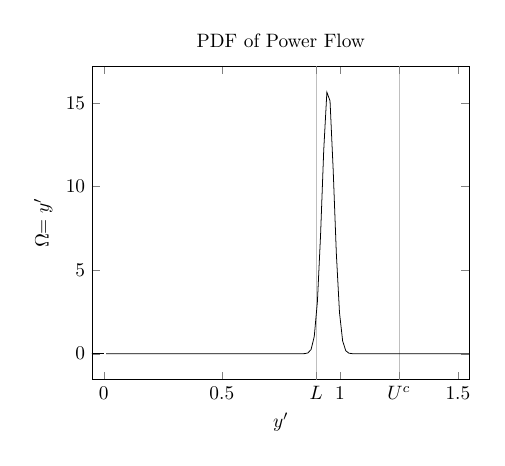
\begin{tikzpicture}[scale=.7]
      \begin{axis}[ title=PDF of Power Flow ,xlabel=$y'$,ylabel=$\bP{\Omega}{\ry=y'}$, xmin=-.05, xmax=1.55, 
          xtick={0,.5,1,1.5},
  	  extra x ticks={.9,1.25},
	  extra x tick style={grid=major},
	  extra x tick labels={$L$,$U^c$}
        ]
        \addplot+[black,no marks,domain=0.01:2,samples=150] { 1/(.025*sqrt(2*3.1415))*exp(-((x-.95)^2/(2*(.025^2))) };
        \addplot+[black,no marks, domain=-2:0,samples=5] {0};
        
      \end{axis}
    \end{tikzpicture}

\end{document}

    \caption{Probability density of power flow}
  \end{subfigure}
  \begin{subfigure}[b]{.445\textwidth}
    \documentclass{standalone}
\usepackage{tikz}
\usepackage{pgfplots}
\begin{document}
    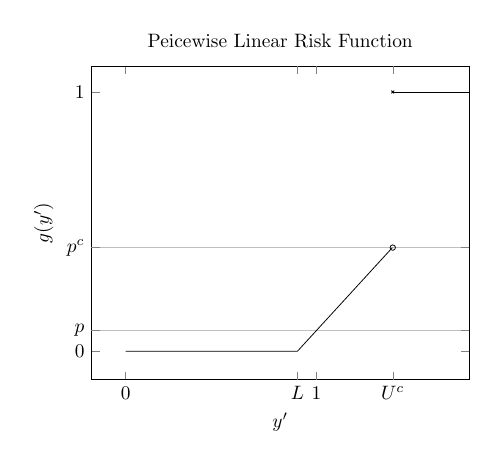
\begin{tikzpicture}[scale=.7]
      \begin{axis}[ 
	  xlabel=$y'$,
	  ylabel=$g(y')$,
	  title = Peicewise Linear Risk Function,
	  unbounded coords = jump,
	  xtick= {0},
	  ytick= {0, 1},
	  extra y ticks={.08,.4},
	  extra y tick style={grid=major},
	  extra y tick labels={$p$,$p^c$},
	  extra x ticks={.9,1,1.4},
	  extra x tick labels={$L$, 1, $U^c$},
          xmax=1.8,
          ymax=1.1,
          scatter/classes={
 	    a={mark=o,line width=3pt,scale=.75},%
 	    b={mark=o,line width=1pt,scale=1.25}%
	}]
	\addplot[black] coordinates { 
	  (0,0)		
	  (.9,0)	
	  (1.3975,.3995)		
	};	
        \addplot[black,mark=x,mark size=1pt] coordinates { (1.4,1) (2.5, 1)};
        \addplot[black,mark=o,mark size=1.4pt] coordinates{(1.4,.4)};
      \end{axis}
    \end{tikzpicture}

\end{document}

    \caption{Failure density versus power flow}
  \end{subfigure}
  \caption{Random Power Flows and the Failure Density Function}
\end{figure}

\subsubsection*{Line Risk Function}
The risk function $g : \R{} \rightarrow \R{}$ takes the normalized flow $\hy_e$ and returns the risk $z_e = g(y_e)$ of the line.  
\begin{equation}
 g(\hy_e) = \bP{\Xi}{\text{Line }e\text{ fails} | \hy_e} 
\end{equation}
A piecewise linear function captures some of the important features of the endogenous risk of the transmission element.  Up to a certain point, $L$, the power flow does not add any risk above that of its normal outage rate.  Above that point, the additional risk is proportional to the additonal flow on the line.  One a critical capacity $U^c$ is reached, a protective element will trip and the line will fail with certainty (ignoring hidden failures).  
\begin{equation}\label{pwl_risk}
g(\hy_e) = \left\{ \begin{array}{l l}
  0 & \hy_e \leq L \\
  a + b \hy_e & L \leq \hy_e < U^c \\
  1 & U^c \leq \hy_e 
\end{array}
\right.
\end{equation}
The risk parameters $(L, p)$ will be fixed among all lines and  $a$ and $b$ can be calculated given the risk parameters $L,p$. 
\endnote{\textbf{Piecewise Linear Function Parameters}

The x intercept snf slope for the line risk function can be calculated as follows.\[a = -\frac{pL}{1-L}\] \[b = \frac{p}{1-L}\]
}
The extension to line specific values is straightforward given the data and could be grouped based off line voltages and material parameters.


\subsubsection*{System Risk Measure}
First, we will define a risk measures in a static setting which can be solved for exactly using nonlinear programming. This risk measure can be weighted to account for importance of lines, which is useful in a cascading failure setting.
\endnote{\textbf{No Cascade Risk Measure}

While it is important that no lines fail, it may be overly restrictive while not actually reducing the risk of large load shedding events, which is the main concern from a system reliability perspective. It would certainly be more beneficial to keep the large high voltage lines in operation that are critical to system stability versus a few small distribution feeders, which may cause some small load shedding but would keep the bad events contained.  In this case, we would like to find the probability of no cascade given a power system operating point.  We can condition this probability on the events of individual lines failing, which we have used previously.
\begin{equation*}
P(\mbox{cascade}|x) = \sum_e P(\mbox{cascade}|e\mbox{ fails}) P(e\mbox{ fails}|x)
\end{equation*}
where $x$ is the operating point and here we worry about the flows $y$ and not the risk from generators.  Let $q_e(y_e) = P(\mbox{cascade}|e\mbox{ fails})$, then we have
\begin{equation} 
H^c(y) = \prod_{e \in \cE} \left( 1 - g_e(y_e)q_e(y_e) \right) \geq 1 - \epsilon
  \end{equation}  
The conditional probabilities $q_e(y_e)$ act as weights on the probability of line failures, so if we set them all to 1 to put an equal importance on every line, we get back our previous formulation.
}
Then, the risk measure is extended to random variables $\rz_e = g( \hry_e )$.


Let $h(z) : \R{M}_+ \rightarrow \left[ 0, 1 \right]$ be the risk function dependent on individual line risk $z$ which is defined by
\[ h(z) = P_\Xi \left[ \mbox{no line fails} \right] \]
where the probability space $\Xi$ is orthogonal to that of demand ($\Omega$) and can be thought of as an effective capacity.  That is, the line will fail if it has flow above its effective capacity.  The space $\Xi$ will then represent transmission elements effective capacity distribution.  

This risk measure defines a bernoulli random variable that takes on the value 1 with probability $h(z)$.  By multiplying the probabilities that individual lines succeed $(1-z_e)$, we have the probability that all lines succeed
\begin{equation}  \label{nofail}
h(z) = \prod_{e \in \cE} \left( 1 - z_e \right)
\end{equation}  
where $z_e$ is the probability that line $e$ fails.  Also, we restrict $z_e \in [0,1)$ since when $z_e = 1$ for any line, we know that the probability no line fails is 0.  This implies that an individual line will have a hard line limit (denoted $U^\epsilon$) related to the system risk $\epsilon$.
\endnote{\textbf{Hard Line Limits}

There is a notion of maximum line limits in this model, however these line limits cannot be attained simultaneously as is true with the current model.  Using the no failure risk measure \ref{nofail} and bounding according to some risk tolerance $\epsilon$, we have
\[ \prod_{e \in \cE} (1-z_e) \geq 1 - \epsilon \]
\[ \sum_{e \in \cE} \ln \left( 1-z_e \right) \geq \ln \left(1-\epsilon \right) \]
where the second constraint is an equivalent formulation using logarithms.
Then we note that all the terms are non-positive, so that the constraint must hold term by term, which gives
\[ \ln \left( 1 - g_e(y_e)  \right) \geq \ln \left( 1- \epsilon \right) \]
\begin{equation*}
g_e(y_e) \leq \epsilon
\end{equation*}
where the second inequality comes from taking exponentials of both sides and reducing. The line will have critical risk $\epsilon$ when $g_e(y_e) = \epsilon$, so that the hard line limits
\begin{equation} \label{hardline}
U^{\epsilon} = g^{-1}\left(\epsilon\right)
\end{equation}
will be an upper bound on line flow.
}
This function can be solved exactly for static demand using nonlinear programming by taking a log transform of the line risk.
\endnote{\textbf{Static Demand, Exact Solution}

The system risk constraint can be written
\begin{equation*} H(y) = \prod_{e \in \cE} \left( 1 - g_e(y_e) \right) \geq 1 - \epsilon
  \end{equation*}  
where $1 - g_e(y_e)$ is the probability that line $e$ doesn't fail given flow $y_e$, and taking the product of all these events gives the probability that no lines fail.  We have
\begin{align*}
  \ln \left( \prod_{e \in \cE}\left( 1 - g_e(y_e)\right) \right) &\geq \ln \left(  1 - \epsilon \right)  & g_e(y_e) \in [0,1) \forall e  \\
  \sum_{e \in \cE} \ln \left( 1-g_e(y_e) \right)  &\geq \ln \left( 1- \epsilon \right) & g_e(y_e) \in [0,1) \forall e 
\end{align*}
Letting $w_e = \ln \left( 1 -g_e(y_e) \right)$ take the value of a transformed line risk, we get our risk constraint
\begin{equation} \label{cceqn}
\sum_{e \in \cE} w_e \geq \ln \left( 1-\epsilon \right)
\end{equation}
with
\begin{align*}
w_e &= \ln \left( 1 - g_e(y_e)\right) \\
e^{w_e} &= 1-g_e(y_e) \\
g_e(x_e) + e^{w_e} &= 1 
\end{align*}
where $e^{w_e}$ is exponential function versus the subscript denoting the line.

And if we wanted to relax the constraint on $w_e$, we have $w_e \leq \ln \left( 1 - q_e(y_e) \right)$ since $w_e$ is related to the probability of success and lowering it would make it worse (and the real number would always satisfy the original constraint).
\begin{equation*}
g_e(y_e) + e^{w_e} \leq 1
\end{equation*}


\begin{figure}
\begin{center} 
\input{\mypathjcc/fig-risksub}
\end{center}
\caption{Line risk substitution for individual branches}
\end{figure}
}

The function can be approximated by using a linearization of $h(z)$,
\endnote{\textbf{Linearization of Line Risk}

To find the linearization for small $t$, the taylor expansion $f(t)=f(t) + \grad f (a)(t-a) +...$ around $a=0$ will be useful.  Applying the taylor expansion to our risk measure \ref{nofail}, we end with the linear approximation
\begin{equation}\label{linear}
h(z) \approx 1 - \sum_e z_e
\end{equation}
%by using the partial derivative of $H(z)$    %%  + \frac{1}{2} (t-a)^T \grad^2 f(a)(t-a)  <---- Quadratic term
%\[ \frac{\partial}{\partial z_{e'}} H ( z ) = \prod_{e \neq e'} (1-z_e) ( -1 )\]
%and $\grad H(0) = -1$.
It is important to note that the linear approximation underestimates system risk and the quadratic approximation overestimates risk for small risk $h(z)$.

The risk can also be bounded using the Bonferroni Inequalities, which is a generalization of Boole's Inequality, or the union bound.
}
which recovers the model used by Wang et. al \cite{wang_2013}.


\subsubsection*{System Risk for Random Variables}
The system risk $r$, which is the probability that one or more lines fail, is the compliment of $h(z)$.  Applying the line risk function \ref{pwl_risk} to the system risk measure \ref{nofail} and integrating over the volatile injection space $\Omega$, we have
\begin{equation*}
1- r = \E{\Omega}{ \prod_{e \in \cE} (1 - g(\hry_e) )}
\end{equation*}
and applying the linear approximation \ref{linear} we get the total risk measure
\begin{equation}
r = 1 - h(z) \approx \sum_{e \in \cE} \E{\Omega}{g(\hry_e)}
\end{equation}
by exchanging summation and expectation of the approximated risk function. 

%\subsubsection*{Expectation of a Truncated Gaussian}
The system risk contributed by line $e$ is integrated over the space orthogonal to exogeneous events.  This will capture the risk from system decision, specifically how much power is flowing through that particular arc.  

\subsubsection*{Line Risk for Gaussian Flows}
Let $ z_e = \E{\Omega}{g(\ry_e)} $ be the individual line risk. We can break $z_e$ into three segments based upon the piecewise linear function \ref{pwl_risk}.  The first segment for $\hry_e \leq L$ takes the value zero, the second segment, for $L \leq \hry_e \leq U^c$, takes an expected value of a truncated normal distribution, and the last segment, $U^c \leq \hry_e$, takes one with a CDF evaluation of a normal distribution.  That is
\[ z_e = \E{\Omega}{ a+b\hry_e | L \leq \hry_e \leq U^c } \bP{\Omega}{L\leq \hry_e \leq U^c}  + \bP{\Omega}{ U^c \leq \hry_e } \] 

 The truncation from the critical capacity $U^c$, the level at which the line fails with certainty, can be ignored since we will stay far away from that point anyway.  This will be a reasonable assumption when $ (U^c - U^{\epsilon} )/\sigma $ is large, where $U^\epsilon$ is the level at which line risk is equal to the system risk tolerance.  Then, we have
\[ z_e = \E{\Omega}{ a+b\hry_e | L \leq \hry_e } \bP{\Omega}{L\leq \hry_e} \]

The branch flows are truncated gaussian, which have known mean and variances.
\endnote{\textbf{Truncated Gaussians}

Truncated gaussian's mean and covariance are known to be
\[  \E{\Omega}{ \hry_e | L \leq \hry_e } = \mu^y_e + \frac{\phi( \alpha_L )}{ 1- \Phi(\alpha_L)} \sigma^y_e \]
\[ \bP{\Omega}{ L \leq \hry_e } = 1 - \Phi(\alpha_L) \]
where $\alpha_L = \frac{L - \mu^y_e}{\sigma^y_e}$, the PDF $\phi(\cdot)$ , and the CDF $\Phi(\cdot)$ are for the standard normal distribution.  
}
The line risk is a function of the mean and covariance of the branch flows.  The line risk expression is then
\begin{equation}\label{line_risk}
z_e(\mu^y_e,\sigma^y_e) = (a + b \mu^y_e)\left[ 1 - \Phi(\alpha_L) \right]  + b \sigma^y_e \phi(\alpha_L) 
\end{equation}
which is a convex function with respect to $\mu^y_e$ and $\sigma^y_e$.
\endnote{\textbf{Convex Line Risk}

The line risk is
\begin{equation}
z_e(\mu^y_e,\sigma^y_e) = (a + b \mu^y_e)\left[ 1 - \Phi(\alpha_L) \right]  + b \sigma^y_e \phi(\alpha_L) 
\end{equation}
Taking the derivatives of $z$ with respect to $\mu^y_e$ and $\sigma^y_e$, we have
\begin{align*}
\frac{\partial z_e}{\partial \mu}(\mu^y_e,\sigma^y_e) & = b\left[ 1 - \Phi(\alpha_L) \right]\\
\frac{\partial z_e}{\partial \sigma}(\mu^y_e,\sigma^y_e) & = b \phi(\alpha_L) 
\end{align*} 
The Hessian is found with the second derivatives and is given by
\begin{equation}
\cH_z(\mu^y_e,\sigma^y_e) = \frac{b \phi(\alpha_L)}{\sigma}
\left[ 
\begin{array}{c c}
1 & \alpha_L \\
\alpha_L & \alpha_L^2
\end{array}
\right]
\end{equation}
Then, we note that the determinant is 0 and the diagonal elements are positive so that there is a positive eigenvalue and a zero eigenvalue, thus the line risk is convex with respect to $\mu^y_e, \sigma^y_e$.  Since system risk is approximated by the sum of line risks, this system risk measure is convex.
}


%%%%%%%% Section 3
\section{Dispatch Models for Bulk Power Systems}
Bulk power systems rely on dispatch models to clear the markets for power in a timely manner.  These models are critical to ensure that market is cleared minimizing cost while maintaining a set of reliability constraints.  In its most common for, the DC power flow model is used to clear economic markets for both real-time and day-ahead operation, where the day-ahead operation has the additional complexity of committing slow ramping resources.  The set of reliability constraints traditionally refer to line thresholds that the system must maintain continuously as well as the systems resiliency to N-1 contingencies.  First, a brief overview of the three models will be given and then the full mathematical programming models for each will be given.  A mention of their extension to exogenous contingencies will be given and then the solution methodology will follow.

\subsection{Overview of Models}
A primary difference between the Optimal Power Flow model and the Joint Chance Constraint model is that the OPF model constrains line risk and the JCC model constrains system risk.  The OPF model is typically done in a static sense where as the JCC model involves uncertainty. The CC model is the extension of OPF under uncertainty.
\begin{description}
\item[Optimal Power Flow (OPF)] This model is used to clear real-time markets for bulk power systems.  It has fixed thresholds for line capacities.  All power flows are assumed to be static.  The regular DC power flow assumptions are used.  The objective is to minimize cost for feasible injects that do not violate line capacity thresholds.
\item[Chance Constraint (CC)] This model assumes a covariance matrix for volatile injects and places probabilistic constraints on line capacity thresholds.  For an arbitrary slack distribution, the standard deviation for line flows can be represent as a second order cone with respect to the slack distribution variables.
\item[Joint Chance Constraint (JCC)] This model replaces line capacity thresholds with line risk measures.  The system risk is the sum of individual line risks.  The objective is to minimize cost for feasible injects that do not violate a system risk threshold.
\end{description}

\subsubsection*{OPF Model}
The OPF model uses the DC simplifications from the full AC model to ensure the model can be solved reliably in a timely manner.  A standard OPF model will be shown here and used for the computational section.
\begin{subequations}
\label{opf_program}
\begin{alignat}{3}
\min_{\left(x,\beta,;\theta,y\right)} && \multispan{2}{$\displaystyle\sum_j \left[  c_2 \left(x_j^2 + \beta_j^2 \sD \right) + c_1 x_j + c_0 \right]$}  & \label{jcc_obj}\\
                        && \textstyle \sum_j c^g_{ij} x_j - \sum_j c^b_{ie} y_e          &=d_i       && \forall i \label{opf_cons}\\ 
                 && y_e - b_e \textstyle \sum_i c^b_{ie} \theta_i          &=0         && \forall e \label{opf_kcl}\\
                 && y_e &\in \left[ -U_e, U_e \right] && \forall e \label{opf_limit}\\
                 && x_j &\in \left[ G^{min}_j, G^{max}_j \right] && \forall j  \label{opf_gen}  \\
                 && \textstyle \sum_j \beta_j &=1 && \label{opf_slack}
\end{alignat}
\end{subequations}

\subsubsection*{CC Model}
The CC model extends OPF to the case with uncertainty in net injects.  The line constraints \ref{opf_limit} will be replaced by probabilistic constraints and additional constraints will be added to describe the slack distribution, standard deviations of branch flows, and probabilistic generator constraint.
\begin{subequations}
\label{opf_program}
\begin{alignat}{3}
                 && y_e + s_e \eta_l &\in \left[ U_e, U_e \right] && \forall j  \label{cc_line}   \\
                 && \pe - \textstyle \sum_j A_{ej} \beta_j   &=0 &&\forall e \label{cc_pi}\\ 
                 && s^2_e - \pi_e^2 \sD + 2 \pi_e \se      &\geq\see &&\forall e \label{cc_var} \\
                 && x_j + \beta_j \sigma_\Delta \eta_g &\in \left[ G^{min}_j, G^{max}_j \right] && \forall j  \label{cc_gen}   \\
                 && \textstyle \sum_j \beta_j &=1 && \label{cc_slack}
\end{alignat}
\end{subequations}
\subsection{Joint Chance Constraint Model}%WITH ARBITRARY SLACK!!
The JCC model departs from traditional power flow models in that it allows for a trade-off between line risk and system risk. Since the cost and risk are both related to the slack distribution, the model will be given with the slack distribution as a variable.  In this section, the full joint chance constraint model will be given followed by a brief explanation of some of the constraints.  The relevant parameters derived from the injection covariance matrix will also be given.  Then a cutting plane algorithm will be shown to solve the full JCC model.

\begin{subequations}
\label{jcc_program}
\begin{alignat}{3}
\min_{\left(x,\beta;\theta,y,\pi,s,z\right)} && \multispan{2}{$\displaystyle\sum_j \left[  c_2 \left(x_j^2 + \beta_j^2 \sD \right) + c_1 x_j + c_0 \right]$} &&\label{jcc_obj}\\
                        && \textstyle \sum_j c^g_{ij} x_j - \sum_j c^b_{ie} y_e          &=d_i       && \forall i \label{jcc_cons}\\ 
                 && y_e - b_e \textstyle \sum_i c^b_{ie} \theta_i          &=0         && \forall e \label{jcc_kcl}\\
                 && y_e &\in \left[ -U_e^\epsilon, U^\epsilon_e \right] && \forall e \label{jcc_limit}\\
                 && x_j + \beta_j \sD \eta_g &\in \left[ G^{min}_j, G^{max}_j \right] && \forall j  \label{jcc_gen}   \\
                 && \textstyle \sum_j \beta_j &=1 && \label{jcc_slack}\\
                 && \pe - \textstyle \sum_j A_{ej} \beta_j   &=0 &&\forall e \label{jcc_pi}\\ 
                 && s^2_e - \pi_e^2 \sD + 2 \pi_e \se      &\geq\see &&\forall e \label{jcc_var}\\
                 && z_e - g(|y_e|,s_e)  &\geq 0 && \forall e \label{jcc_lr}\\
                 && \textstyle \sum_e z_e &\leq \epsilon && \label{jcc_risk}
\end{alignat}
\end{subequations}

The objective \ref{jcc_obj} for the JCC model is the typical quadratic objective for the OPF model plus a contribution from the slack distribution due to the uncertainty in the volatile injects.  This objective is the expected cost of meeting the realized demand.  The uncertainty in demand also causes the generator constraint \ref{jcc_gen} to be probabilistic with $\eta_g = \Phi^{-1}(1-\epsilon_g)$ being its tolerance.  The upper and lower bounds $[G^{min},G^{max}]$ will be dependent on many things, most importantly the time frame used.  This will be affected by the status of the generator (on,off,starting up,shutting down) and its ramping rate as well as any physical limits it may have.  

The first equations \cref{jcc_obj,jcc_cons,jcc_kcl,jcc_slack,jcc_limit,jcc_gen} are your typical DC power flow and the last set \cref{jcc_pi,jcc_var,jcc_lr,jcc_risk} describe system risk.  The branch variance equations \ref{jcc_var} are a second order cone and the line risk equations \ref{jcc_lr} involve the CDF of a normal distribution.  These equations will be solved via a cutting plane approach so that the individual subproblems will be linear programs.


\subsubsection*{Branch Response Parameters}
The volatile injects have mean 0 and a covariance matrix $\Sigma^m$.  This covariance matrix is used to describe parameters for relating the injection covariance matrix to the branch covariance matrix needed for line risk.  The variance in lines is due to a combination of the volatile injects and the slack distributions response.  The following parameters are used in JCC \ref{jcc_program} and the cutting planes \ref{branch_var_cuts}.
\begin{subequations}
\begin{align}
 \sD &= \sko \skt \sigot  \\
 \se &= \sko \skt A_{ek_1} \sigot \\
 \sen &= \sko \skt A_{ek_1} A_{nk_2} \sigot
\end{align}
\end{subequations}


\subsection{Exogenous Contingencies}
The JCC model also has a straightforward extension to exogenous contingencies.  In the computational experiments, each model will have a respective N-1 version which ensures the system is stable after any single line goes out.  In order to explore this model, line outage factors are used, which are linear shift factors for branch flows.  Using these, constraints will be formed on the second stage branch flow variables.  The mean branch flow as well as standard deviation of flow can be calculated.  In the OPF version, hard line constraints are used.  In the CC version, probabilistic constraints are formed for line flow.  Finally, the JCC version enforces a system risk constraint on each N-1 subsystem.  In all versions, the respective constraints are loosened in the second stage.

The implementation as well as solution method, which closely parallel the base case, are given in the notes.
\endnote{\textbf{Exogenous Contingency Details}


The mean branch flows for line $e$ given contingeny $n$ can be found by
\begin{equation}
 \ry_e^n = \ry_e + L_{e n} \ry_n 
\end{equation}
with $L_{en}$ being a line outage factor for outage $n$'s effect on line $e$.
\textbf{Line Outage Factors}
The line outage factor can be found by first finding the branch sensitivity matrix and then apply a scale so that when the line outage factor is multiplied by the current branch flow, the response to all other branches is found.
\begin{equation}
L_{en} = \left\{ \begin{array}{c c}
  -1 & \mbox{ if } e=n\\
  A_{en}^B (1-A_{nn}^B)^{-1} & \mbox{ if } A_{nn}^B \neq 1\\
  \mbox{NaN} & \mbox{ o/w }
  \end{array}
\right.
\end{equation}

In addition, the standard deviation of branch flows can be calculated.  The variance of branch flows are
\begin{equation}
 Var[\ry_e^n] = Var[\ry_e] + L^2_{e n} Var[ \ry_n ] + 2 L_{e n} CoVar[ \ry_e, \ry_n ]
\end{equation}

\textbf{Joint Chance Constraints for N-1 Security}

The following equations are added to JCC to define JCC N-1.
\begin{subequations}
\label{jcc_program}
\begin{alignat}{3}
y^+_{en} - y_e - L_{en} y_n & \geq 0 && \forall e,n\\
y^+_{en} + y_e  +  L_{en} y_n & \geq 0 && \forall e,n\\
 s_{en}^2 - \psen^2 \sD + 2 \psen \left( \se + L_{en} \sn \right) &\geq \sigma^2_{\psi_{en}} && \forall e,n\\
z_{en} - g(y^+_{en},s_{en}) &\geq 0 && \forall e,n\\
\sum_e z_{en} &\leq \epsilon_n && \forall n
\end{alignat}
\end{subequations}

Shift factors for multiple lines can be found provided certain conditions are met. \cite{guler_2007}

The effect of the outage of line $n$ has on line $e$ is related to $\psen$, which can be calculated as
\begin{equation}
 \psen = \pe + L_{en} \pn
\end{equation}

The injection covariance matrix allows you to calculate this parameter which is used in the branch covariance matrix and cutting plane algorithms.

\textbf{Branch Response Parameter}
\begin{equation}
\sigma^2_{\psi_{en}} = \sko \skt \left(A_{ek_1} + L_{en} A_{nk_2}\right)^2 \sigot
\end{equation}

The cutting planes for N-1 are
\begin{align*}
s_en \geq \fenb &+ \sum_j \pfenb \left( \beta_j - \hat{\beta_j} \right)\\
\fenb &= \sqrt{ \psen^2 \sD - 2 \psen \left( \se + L_{en} \sn \right) + \sigma^2_{\psi_{en}}} \\
  \pfenb &= \frac{\left(A_{ej} + L_{en}A_{nj}\right) \left( \psen \sD - \left(\se + L_{en} \sn \right) \right)}{\sqrt{\psen^2 \sD - 2 \psen \left(\se  + L_{en}\sn \right) + \sigma^2_{\psi_{en}} }}
\end{align*}
}

\subsection{Solution Method}
Due to the inclusion of non-analytic functions (the line risk function), an out of the box solver would not work.  However, the risk function is convex, so cutting planes were chosen for the solution methodology.  In addition, there were many second order cone constraints (number of lines).  Instead of using these constraints explicitly, they were added indirectly through cutting planes as well.  This kept the program to a manageable size and allowed for fast solve times.  When exogenous contingencies are added, cutting planes are extremely efficient since no constraints will be added for lines without risk.


\subsubsection*{Risk Function for Transmission Lines}
The line risk constraint \ref{jcc_lr} involving the CDF function for a normal distribution rules out many potential solving options.  Since the equations are convex, we can solve this using a cutting plane approach to describe the line risk in terms of the mean branch flow $y_e$ and the standard deviation of branch flow $s_e$.  While there are infinitely many cuts, this program can be solved for a given error tolerance with a finite, and typically small, set of cuts.
\begin{subequations}
\label{line_risk_cuts}
\begin{align}
z_e \geq g(\hye,\hse) &+ \frac{\partial g}{\partial y_e}(\hye,\hse) \left(y_e - \hye \right) 
+ \frac{\partial g}{\partial s_e}(\hye,\hse) \left(s_e - \hse \right) \\
g(y_e,s_e) &= (a + b y_e)\left[ 1 - \Phi(\alpha_L) \right]  + b s_e \phi(\alpha_L)  \\
 \frac{\partial}{\partial y_e}g(y_e,s_e) &= b\left[ 1 - \Phi(\alpha_L) \right]\\
\frac{\partial}{\partial s_e}g(y_e,s_e) &= b \phi(\alpha_L) 
\end{align}
\end{subequations}


\subsubsection*{Branch Variance Constraints}
The standard deviation of branch flow can be formulated as a second order cone with respect to the slack distribution variables.  While this could be solved with an out of the box solver, we proceed with a cutting plane approach to speed up solve times.  As the solution approach is already iteratively improving system risk, it adds only a small amount of work to add these cuts as well.
\begin{subequations}
\label{branch_var_cuts}
\begin{align}
s_e \geq \fehb &+ \sum_j \pfehb \left( \beta_j - \hat{\beta_j} \right)\\
  \feb &= \sqrt{\pe^2 \sD - 2 \pe \se  + \see }\\
  \pfeb &= \frac{A_{ej} \left( \pe \sD - \se \right)}{\sqrt{\pe^2 \sD - 2 \pe \se  + \see }}
\end{align}
\end{subequations}


\subsubsection*{Cutting Plane Algorithm}
Now, we can describe the cutting plane algorithm for JCC at a high level and give pseudo-code \ref{jcc_alg} for implementation.  The main subproblem the algorithm will solve is the standard DC power flow.  After solving, the generator injects $x$, slack distribution $\beta$, and branch flows $y$ will be used to calculate risk information about the dispatch point.  To get the risk information, the branch standard deviations $s$ need to be calculated.  With the mean flow $y$ and standard deviation $s$, the line risk $z$ can be calculated.  The sum of line risk is system risk $r$.  If $r$ is less than the required system risk $\epsilon$, the problem is solved.  Otherwise, the algorithm will add cuts for all lines with a positive risk $z$.  The cuts will describe how $z$ is related to $y,s$ and how $s$ is related to $\beta$.  Then the power flow subproblem will be solved with the addition of the cuts and this will repeat until it is infeasible or the risk constraint is satisfied.
\begin{algorithm}
\caption{This cutting plane algorithm solves JCC \ref{jcc_program} via linear programs and cutting planes}\label{jcc_alg}
\begin{algorithmic}
\Procedure{JCC}{d,$\Sigma^m$,$\epsilon$,$\epsilon_g$,L,p}
\State $L \gets \emptyset$  (Set of Lines with potential risk)
\State $S \gets \emptyset$  (Set of Cuts)
\State $r \gets 0$ (Risk)
\BState \emph{solve}:
\State $(\hat{x},\hat{\beta},\hat{y}) \gets $Solve DC Power Flow, \cref{jcc_obj,jcc_cons,jcc_kcl,jcc_slack,jcc_limit,jcc_gen}, with cuts $S$, risk $r\leq\epsilon$
\If {Infeasible} \Return Problem Infeasible 
\EndIf
\State Calculate $\hat{s},\hat{z},\hat{r}$ using $(\hat{x},\hat{\beta},\hat{y})$ and \cref{branch_cov,line_risk}
\If {$\hat{r} \leq \epsilon + tol$} \Return Optimal $(\hat{x},\hat{\beta},\hat{y},\hat{s},\hat{z},\hat{r})$
\EndIf
\For{$\forall e$}
\If {$\hat{z_e} \geq tol$}
    \If {$e \notin L$}
            \State $L \gets \left\{L,e\right\}$
            \State Initialize $s_e,z_e$
            \State $r \gets r + z_e$
    \EndIf            
    \State $S \gets$ line risk cuts \ref{line_risk_cuts} for $z_e,y_e,s_e$ dependent on $\hat{z}_e,\hat{y}_e,\hat{s}_e$
    \State $S \gets$ branch variance cuts \ref{branch_var_cuts} for $s_e,\beta_e$ dependent on $\hat{s}_e,\hat{\beta}_e$
\EndIf
\EndFor
\State \textbf{goto} \emph{solve}
\EndProcedure
\end{algorithmic}
\end{algorithm}




%%%%%%%% Section 5
\section{Computational Experiments}
This section will explain the computation setup, the test cases, the experiments performed, and the intuition to gain from the comparison of OPF, CC, and JCC models.
\subsection{Implementation of the JCC Model}
All of the experiments are run on a laptop with an Intel i7-3537U processor with 2 cores,4 threads at 2.00GHz.  The laptop has 8GiB of memory, but even with the large case files (2383 nodes), memory is not an issue.  The laptop is running Linux Mint Petra 16.  The OPF, CC, and JCC models are all solved within a C++ program.  The program uses Armadillo\cite{armadillo} for linear algebra and Concert and CPLEX to solve the linear programs.  CPLEX is run with default settings and the dual simplex algorithm is used to solve the linear programs (quadratic objective for the small case).  All time comparisons are using the same system environment with a fixed clocked speed and few programs in background.  The primary DC OPF solver in the C++ program has been developed to output nearly identical results to Matpower.\cite{matpower} 
\subsection{Single Instance}
The test cases are all pulled from Matpower test cases.  The two test cases used will be the 30 bus test case as well as the 2383wp test case.  The small test case will be used to show some properties of the different dispatch points and the cost-risk frontier.  The large test case will be used for time trials as well as a cost-risk scatter plot.  

\subsubsection*{30 Bus Case}
This case from Matpower has 30 buses, 41 branches, and 6 generators.  The branches have a single capacity rating and in the given demand scenario does not have active line constraints.  A capacity factor $M$ will be used to uniformly scale the branch capacities.  All of the generators are active and have quadratic cost functions.  Ramping constraints for generators are not considered and the generators are allowed to take any value in its given range (the probabilistic generator constraints are ignored to focus on branch constraints).  In addition, all generators will be allowed to participate in the slack distribution.  Each bus with a demand will be considered volatile, with mean equal to the demand.  For this example, the injections will be independent of each other but this need not be the case.  The variance of each injection is equal to 5\% of the demand at the node times a budget factor $B$.

\begin{table}
\centering
\begin{tabular}{ |c| c c c |}
\hline
& OPF & CC & JCC \\
\hline
\hline
Cost & 567.1 & 574.0 & 565.2\\
$r$ & 0.0171 & 0.0179 & 0.0080\\
\hline
\end{tabular}
\caption{Cost and risk results for OPF,CC, and JCC models on the small test case}\label{solve_results}
\end{table}

\begin{table}
\centering
\scriptsize
\begin{tabular}{| c| c |c c c c c c |}
\hline
 & Mod & g1 & g2 & g3 & g4 & g5 & g6 \\
\hline
\hline
$\left[ g_{min}, g_{max} \right]$& & [0,80]&[0,80] &[0,50] &[0,55] &[0,30] &[0,40]  \\
$\left\{ c_2, c_1 \right\}$ && $\left\{0.02,2\right\}$  &$\left\{0.0175,1.75\right\}$ &$\left\{0.0625,1\right\}$ &$\left\{0.00834,3.25\right\}$ &$\left\{0.025,3\right\}$ &$\left\{0.025,3\right\}$  \\
\hline
\hline
$x_g$ &OPF& 39.7  &  52.3  &  24.2  &  35.7  &  19  &  18.3   \\
$x_g$ &CC& 35.9  &  47.9  &  25.7  &  37.2  &  19.3  &  23.1    \\
$x_g$ &JCC& 41.9  &  55.0  &  23.2  &  34.0  &  18.6  &  16.5    \\
\hline
$\beta_g$ &OPF& 0.1548  &  0.1769  &  0.0495  &  0.3712  &  0.1238  &  0.1238    \\
$\beta_g$ &CC& 0  &  0  &  0.4411  &  0.2986  &  0  &  0.2602   \\
$\beta_g$ &JCC& 0.2456  &  0.2795  &  0.0846  &  0.0646  &  0.0597  &  0.2659   \\
\hline
\end{tabular}
\caption{Generator results using OPF, CC, and JCC models on the small test case.}\label{solve_one}
\end{table}

The first example will have risk parameters $L=0.9$, that is a line will begin taking on risk after it is at 90\% of its rated capacity.  The factor $p=0.005$ means that at nominal capacity, the line will have a $0.5\%$ chance of failing.  The line capacities will be scaled by $M=0.745$. The system risk constraint will be $\epsilon=0.008$, that is a $0.8\%$ chance of one or more lines failing.  The chance constraint version of OPF will be defined by $\eta_L=0.05$, that is the line capacities can not be violated more than $5\%$ of the time.  Finally, the covariance matrix will be scaled by $B=0.025$ so that the stanadard deviation of aggregate demand is $0.6$, a small fraction of total demand $189.2$.  The results for $(x,\beta)$ are tabulated in \cref{solve_results,solve_one}.



The CC model is always more conservative then the OPF model as it will tighten the line constraints.  This means that the CC version will always be at least as expensive as the OPF model.  In this case, the total cost rose by \$7 to ensure the line constraints were met probabilistically (95\% of the time).  The JCC model was able to lower the cost because it removed the branch capacity constraints (or increased them by 6\% to match the system risk level).  In addition, JCC knows and constrains the system risk measure so that it is able to find a cheaper point with a system risk level half that of the OPF and CC models.



Another interesting feature is that the slack would like to be distributed as much as possible to reduce cost.  This can be seen from the objective \ref{jcc_obj} due to the squared beta term and the OPF results show it spreading when there is no concerns of line or system risk.  The CC model slightly changes it's generator position as well as removing 3 generators from the slack distribution.  It is removing generators which have an effect on the probabilistically constrained transmission lines in order to ensure that the constraints are met $95\%$ of the time.  The JCC model has moved in almost exactly the opposite direction and has kept a distributed slack.


\subsection{Cost-Risk Frontier}
  \begin{figure} 
\centering
\documentclass{standalone}
\usepackage{tikz}
\usepackage{pgfplots}
\begin{document}
\begin{tikzpicture}
\begin{axis}[title=Cost vs Risk (case30),scale=1, xlabel=Cost, ylabel=Risk, legend pos=outer north east]
\addplot+[opacity=.7,mark size=1] table[x=copf,y=ropf] {\mypathjccdata/cost-risk2.dat};
\addlegendentry{OPF}
\addplot+[opacity=.7, mark size=.1] table[x=ccc,y=rcc] {\mypathjccdata/cost-risk2.dat};
\addlegendentry{CC}
\addplot+[opacity=.7, mark size=.1] table[x=csjc,y=rsjc] {\mypathjccdata/cost-risk2.dat};
\addlegendentry{JCC}
\end{axis}
\end{tikzpicture}
\end{document}
%pow case/30.db  .775 1.1 1 .00195 .4 .00275 .5 .9 .005 .4 1000 2> cost-risk.dat
%m0   m1          mg   eps epsN     pL pG     L  p  B    T
%0.775            1.1  1   0.00195  0.4       0.00275    0.5     0.9     0.005   0.4     1000

\caption{Reliability frontier for the small test case}\label{costriskfront}
\end{figure}

Now we will use this same example case to draw a cost-risk frontier.  An efficient operating point would be at that boundary of the feasible points, that is, neither cost nor risk can be improved without a loss to the other.  Since neither the OPF or CC model uses or constrains our risk measure, it would be unlikely for them to be on the boundary.  In figure \ref{costriskfront} we see that this is the case.  The OPF model is in the interior and is equivalent to the CC model when $\eta_l=.5$.  Since the branch flows are gaussian, if the mean flow is at its threshold, it has a 50\% chance of being over its threshold.  As $\eta_l$ is reduced, the CC line is drawn.  The JCC line is started by finding the point when the system risk level is not constrained, for this case $r=.01$.  As $r$ is decreased, the system risk becomes constrained and the cost begins to rise as the risk level is reduced.


It is important to note that the cost-risk frontier is entirely dependent on how system risk is measured.  In our case, we use a piecewise linear failure density function with parameters $L$ and $p$.  As $L$ and $p$ are varied, the shape of these frontiers will change.  Holding $p$ fixed and increases $L$ towards 1, the CC model, while still on the interior of the frontier, does a better job of reducing system risk.  With $L$ around .98 (this will depend on the variance of aggregated injects), the CC and the JCC behave similar.  Both programs will try to reduce the flow of lines that are at their capacity, with the exception that JCC will allow a small number, typically one, of these lines to increase.  More discussion on this behavior will be given in the sensitivity analysis section \ref{senseanal}


\subsubsection*{2383wp Bus Case}
This case from Matpower has 2383 buses, 2896 branches, and 327 generators.  The case is similar to the small case in many respects, such as only a single line rating capacity being given.  The generators have the biggest difference in that there are many which are nearly fixed and have no cost.  The larger flexible generators are only given a linear cost so that there is no quadratic objective.  The covariance matrix will be developed the same as in the small case.

Running this case with parameters $M=1.03, \epsilon=0.03, \eta_L=0.05, L=0.85, p=0.005$, and $B=1$ and recording the standard cost and risk information as well as solve time.  The case was repeated 10 times and the mean time is reported in \ref{solve_time}.  CC and JCC take a similar amount of time, the majority of the work at each step being the calculation of the branch covariance matrix.  The total time will largely depend on how many iterations the algorithms take, which is typically around 5-7. 

In addition, we solved 100 instances with random demand and the same covariance matrix to show the speed-up you can achieve with repeated solves.  By having the same covariance matrix, all of the cuts for previous solves are still valid.  So, in addition to using a warm start on the LP, after the first few solves the algorithm typically needs no additional cuts.

\begin{table}
\centering
\begin{tabular}{| c| c c c| }
\hline
Time ($\eta_L,\epsilon$) & OPF & CC & JCC \\
\hline
\hline
Time (0.05,0.03)& 0.37  & 8.7 & 7.5 \\
%Time (0.10,0.05)& 0.37 & 8.6  & 7.4  \\
Time (0.20,0.07)& 0.37  & 8.4 & 8.0 \\
%Time (0.30,0.10)& 0.37  & 8.4 & 7.6 \\
Time (0.40,0.20)& 0.37  & 8.3 & 6.1 \\
%Time (0.45,0.30)& 0.37  & 8.3 & 6.1 \\
Time (0.48,0.30)& 0.37  & 7.7 & 6.1 \\
\hline
\hline
Avg Time (100 trials)& 0.34  & 2.2 & 2.3 \\
\hline
\end{tabular}
\caption{Time comparison, in seconds, for OPF,CC, and JCC on the large test instances.}\label{solve_time}
\end{table}


\subsubsection*{Line Threshold Comparison}
Here we will explore what the JCC model is doing to lower its cost or risk compared to the traditional models.  For this experiment, the parameters are as follows, $M=1.03, \epsilon=0.015, \eta_L=0.05, L=0.95, p=0.005$, and $B=1$.  Solving this program, we see that the majority of the lines are less than 50\% utilized.  There is a small number of lines that are at or near their nominal capacity.

\begin{figure}
\begin{tabular}{c c}
\documentclass{standalone}
\usepackage{tikz}
\usepackage{pgfplots}
\newcommand{\mypathjcc}{../jcc}
\newcommand{\mypathjccdata}{../jcc/data}
\begin{document}
\begin{tikzpicture}[scale=.8]%1.3,1
\begin{axis}[title=Normalized Line Flow , xlabel=Line, ylabel=Line Flow (MW),xmin=0,xmax=9, grid=major]

                        \addplot+[opacity=.9,only marks, mark size=1, mark=triangle,
                        /pgfplots/error bars/.cd,
                        x dir=none,
                        y dir=both,
                        y explicit] table[x=count,y=opf, y error=eopf] {\mypathjccdata/highflow.dat};
                        \addlegendentry{OPF}

                         \addplot+[opacity=.9,only marks, mark size=1, mark=o,
                        /pgfplots/error bars/.cd,
                        x dir=none,
                        y dir=both,
                        y explicit] table[x=count,y=cc, y error=ecc] {\mypathjccdata/highflow.dat};
                        \addlegendentry{CC}

                        \addplot+[opacity=.9,only marks, mark size=1, mark=square,
                        /pgfplots/error bars/.cd,
                        x dir=none,
                        y dir=both,
                        y explicit] table[x=count,y=sjc, y error=esjc] {\mypathjccdata/highflow.dat};
                        \addlegendentry{JCC}

\end{axis}
%\begin{axis}[hide x axis, axis y line=right,ymin=-50,ymax=950,xmin=0,xmax=9,ylabel=Shadow Price (\$)]
%   \addplot+[only marks,mark size=4,mark=star] table[x=count,y=dual] {\mypathjccdata/duals.dat};
%   \addlegendentry{Shadow Price (OPF)}
%\end{axis}
\end{tikzpicture}
\end{document}

&
\documentclass{standalone}
\usepackage{tikz}
\usepackage{pgfplots}
\begin{document}
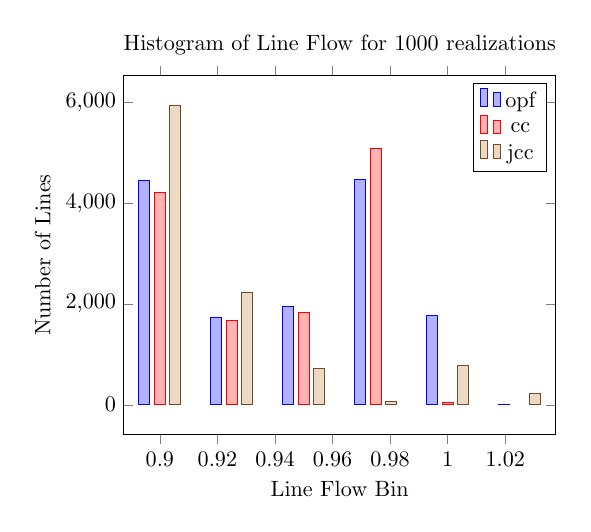
\begin{tikzpicture}[scale=.8]
\begin{axis}[title=Histogram of Line Flow for 1000 realizations, 
    xlabel=Line Flow Bin, 
    ylabel=Number of Lines,
x tick label style={
/pgf/number format/1000 sep=},
  ybar, bar width=5pt ,
  enlargelimits=0.1]
\addplot coordinates { ( 0.9,4450)  ( 0.925,1729)  ( 0.95,1949)  ( 0.975,4471)  ( 1,1770)  ( 1.025,3) };
\addplot coordinates { ( 0.9,4219)  ( 0.925,1678)  ( 0.95,1834)  ( 0.975,5077)  ( 1,53) };
\addplot coordinates { ( 0.9,5931)  ( 0.925,2218)  ( 0.95,711)  ( 0.975,70)  ( 1,784)  ( 1.025,221) };
\legend{opf,cc,jcc}
\end{axis}
\end{tikzpicture}
\end{document}

\end{tabular}
\caption{Top lines resulting in congestion based risk}
\end{figure}


Now, we will look at the trade off that the JCC model is able to make due to it increasing the nominal line limit by 10\% to match the given system risk level.  In figure \ref{solve_shadow}, 8 lines are shown, which are lines above 95\% of their nominal capacity in the OPF model.  The mean line flows are plotted as well as the standard deviation based on the slack distribution for the solution.  
%There are 8 lines above 95\% of their capacity in the OPF model, indexed as lines 23,291,320,1380,1381,1815,2108, and 2109. 
In addition, the shadow prices for the original OPF model are shown for lines that are constrained.  In the OPF model, there are 3 lines at the nominal capacity.  Line 23 (index 1 in figure) has a dual price of 872, line 291 (index 2) has a dual price of 32, and line 2108 (index 8) has a dual price of 294.


In the CC model, these constraints are tightened further to ensure that these thresholds are met at least 95\% of the time.  The JCC model on the other hand relaxes these constraints and imposes a system risk constraint instead.  The final solution for the JCC model will have line 23 exceed its threshold with certainty but is rewarded with the high shadow price.  On the other hand, other lines with positive line risk may be restricted to ensure the system risk levels are met.

To give another perspective, the line flows were sampled and binned to create a histogram of line flows to show the trade-off between models.  For the JCC model, the line risk parameter $L$ was chosen to be 0.9.  The results can bee seen in figure \ref{histogram} where the bin size is $0.025$, for example the point $1$ is in reference to bin $1$ to $1.025$.  We can see that the normalized line flows pile up in bin 0.975 for the CC model and there are a number of lines in OPF that are in bin $1-1.025$, thus exceeding their capacity a significant amount of the time.  The JCC also has a line that exceeds its capacity, almost with certainty.  However, the JCC has far fewer lines that are at or near their capacity.



\subsection{Sensitivity Analysis}\label{senseanal}
Now, we want to look at the sensitivity of the JCC models to its input parameters and demand uncertainty.  First we will look at how the risk of the different dispatch points from the OPF, CC, and JCC models respond to changes in the failure density function parameters $L$ and $p$.  To this end, we solved the OPF, CC ($\eta_L=.01$), and JCC ($\epsilon=0.0003$, $L=.98$).  These three dispatch points are used to find the risk of the branch flows for varying risk parameters $L,p$. The cost of the dispatch points are tabulated in \ref{tabsense} and the sensitivity analysis is shown in figure \ref{figsense}. This figure shows that for the given JCC solution, the system risk stays under that of the CC model.  The OPF model has a lower cost so it is reasonable that the risk is much higher.  The same results were seen when polynomial risk functions were evaluated, such as $x^2,x^3,$ and $x^4$.


\begin{table}
\centering
 \begin{tabular}{ |c| c c c |}
\hline
& OPF & CC & JCC \\
\hline
\hline
Cost & 567.1 & 574.0 & 572.2\\
\hline
\end{tabular}
\caption{Table of cost for the three dispatch points used in the sensitivity analysis}\label{tabsense}
\end{table}


\begin{figure}
\centering
\documentclass{standalone}
\usepackage{tikz}
\usepackage{pgfplots}
\begin{document}
\end{document}

\caption{A comparison of the three dispatch points for varying risk function parameters}\label{figsense}
\end{figure}


\begin{verbatim}
pow  case            m0  m1 mg eps epsN eta etaG L p  B   T
pow case/30.db  .77 1.1 1 .00021 .4 .01 .5 .98 .005 .4 10000
pow case/30.db  .77 1.1 1 .0028 .4 .01 .5 .9 .005 .4 10000
pow case/30.db  .77 1.1 1 .0046 .4 .01 .5 .8 .005 .4 10000
pow case/30.db  .77 1.1 1 .0046 .4 .05 .5 .8 .005 .4 10000
\end{verbatim}
%solvesensitivty

\begin{table}
\centering
 \begin{tabular}{ |c| c c c c c c|}
\hline
& OPF & CC .01 & CC .05 & JCC .98 & JCC .9 & JCC .8 \\
\hline
\hline
Cost & 565.215 & 590.172 & 572.833& 589.594 & 581.92 &579.135\\
%$r$ & 0.00504327 & 0.0015044 & 0.0169355 & 0.000309812 &.0028877 &0.00466\\  -- shown in picture
\hline
\end{tabular}
\caption{Sensitivity Analysis Results}
\end{table}


\begin{table}
\centering
\begin{tabular}{| r  c |}
\hline
Risk :& Ex[$y_e > U_e$] \\
\hline
\hline
OPF:& 0.3875\\
CC .01:& 0.0225\\
CC .05:& 0.1971 \\
JCC .8:& 0.31 \\
JCC .9:& 0.09 \\
JCC .98:& 0.0125 \\
\hline
\end{tabular}
\caption{Expected number of lines over their threshold}
\end{table}

\begin{figure}
\documentclass{standalone}
\usepackage{tikz}
\usepackage{pgfplots}
\newcommand{\mypathjccdata}{../jcc/data}
\usepackage{amsmath,amssymb,amsfonts} % Typical maths resource packages
\input{def}
\newcommand{\ry}{\pmb{y}}
\begin{document}

\begin{tikzpicture}[scale=.8]
\begin{axis}[title=L vs Risk, xlabel=L, ylabel=r,legend pos=outer north east,ymax=.04,xmin=.9,xmax=1,
	  extra x ticks={.98},
	  extra x tick style={grid=major},
	  extra x tick labels={}]


  \addplot+[opacity=.65,only marks, mark size=.35] table[x=L,y=ropf] {\mypathjccdata/risk.dat};
  \addlegendentryexpanded{OPF}

  \addplot+[opacity=.65,only marks, mark size=.35] table[x=L,y=rcc] {\mypathjccdata/risk.dat};
  \addlegendentryexpanded{CC}

  \addplot+[opacity=.65,only marks, mark size=.35] table[x=L,y=rsjc] {\mypathjccdata/risk.dat};
  \addlegendentryexpanded{JCC}

\end{axis}
\end{tikzpicture}
\end{document}

\caption{Sensitivity analysis for other polynomial risk functions}
\end{figure}


%%%%%%%% Section 6
\section{Going Forward}

\subsection{Model Strengths}
The primary strength of this model is the addition of a system risk constraint and the removal of line thresholds. Line thresholds are hard constraints that subject the system to price spikes.  The hard line constraints are somewhat arbitrary as the line will not fail when it is exceeded by a small amount.  Instead, an economic trade off should be made between individual lines to ensure the system risk is constrained at an adequate level.  The system risk measure allows for direct comparison of different dispatch points with respect to risk.

The JCC model is computationally efficient in its full form.  It allows for creation of a cost-risk frontier that finds dispatch points that are better in both terms of risk and cost.  Under uncertainty, this model should be compared against the CC model, which is a probabilistic interpretation of line thresholds.  Probabilistic line thresholds exacerbate the economic problems of hard constraints by further tightening the constraints.  In both of these models, the variable slack distribution plays a small direct role in cost through the objective, however is crucial in ensuring the line and system risk constraints are met.  
  
Combining the system risk measure and random power injects for the joint chance constrained model accounts for many things the traditional OPF model misses.  This model will give prices for system response to aggregated volatile injects, which is regulation and reserve support for different time periods.  Instead of having an ancillary service model which separates this, the JCC model directly accounts for it.  This will allow for valuing volatile injects, which will be important going forward as the grid integrates more uncertain generation (wind turbines) and demand (electric vehicles).

\subsection{Possible Extensions}
There are many avenues to improve and extend this model.  One first question would be, what does the failure density function look like.  We used a piecewise linear model, but perhaps other models better represent the true physics of the situations, such as a polynomial, ie $x^2$.  In addition, often the effective capacities are correlated.  Effective capacities are related to environmental conditions, such as high wind, which are geographically correlated.  During high wind periods, there is increased wind generation as well as increased effective capacities, which means that when the turbines are producing more energy, the nearby transmission lines are also capability of carrying more energy.  Finally, the volatile injects need to be priced and accounted for.  Volatile injects add stress to the grid which needs to be secured through additional resources.  These injects should bear the cost of the stress they add to the system.


\theendnotes

\setcounter{endnote}{0}

%\newcommand{\mypathslk}{../thesis/slk}
\chapter{Slack Market for Price Risk Reduction}

\section{Slack Market}


\chapter{Conclusion}
\section{Contributions}
The first chapter's primary contribution was to model the existing cascading power failure simulation as a multi-stage stochastic program using mixed integer variables.  The primary difficulty was overcoming the decision dependent uncertainty, which was done by using the concept of effective capacity distribution and a priori sampling.  While the computational difficulty made practical use of this impossible, if highly probable sequences of failures were known in advance, this model could be used to protect against them.

The second chapter's primary contribution was to optimize over the OPA simulation efficiently, which previously was only used in simple sensitivity analysis.  To this end, an efficient implementation was made with a common random number scheme to reduce variance and low system requirements to allow for massively parallel solution methodology.  In addition, DFO techniques were used to filter the high frequency noise and exploratory steps using accessory information from the OPA simulation enhanced the solution time to allow for large test case optimization.

The third chapter's primary contribution was to develop a dispatch model that included a system risk constraint to control endogenous risk from line loading.  This system risk measure was modeled as a joint chance constraint and can be calculated analytic even under net injection uncertainty.  The cost-risk frontier was explored and the new model was compared to the standard chance constraint model used in recent literature.  The chance constraint model can be closely replicated with the JCC model, however it is inefficient according to our system risk metric and the JCC model is far more flexibile.

\section{Future Work}
The primary research going forward will be finalize the DFO implementation for the OPA simulation and develop extensions to the JCC model for pricing and reliability analysis.
\begin{itemize}
\item Optimizing Design Problems (Ch. 3)
\bi
\item Implement full DFO algorithm and explore effects from using problem specific information
\item Compare direct search method with model based method for DFO algorithm
\ei
\item Risk Model for Real-Time Dispatch (Ch. 4)
\bi
\item Make use of the extension of JCC to exogenous contingencies by measuring the relability of the system using the OPA cascading model
\item Price the covariance matrix for net injection uncertainty using the shadow prices from the system risk constraints in the JCC model.
\ei
\end{itemize}

Currently, only brute force exploration procedures were used in the parallel framework developed for optimizing over the OPA simulation.  This was used to understand the accessory information gained from the solution such as intermediate line flow and load shed data.  Now, direct search and model based search procedures will be implemented and compared.  These search procedures will be enhanced with problem specific information to speed up solve times.

The JCC model will be extended to allow for pricing the covariance matrix for net injection uncertainty.  This uncertainty is responsible for a large portion of system stress that is protected against using ancillary services such as regulation and reserves.  By pricing this, the assets and injection points responsible for this stress will be charged in order to send proper price signals through the market.

In addition, the JCC model will be used for a decision policy in the first two stages of the OPA cascade, replacing the standard DC power flow decision policy.  This will be done to explore the effects the JCC model will have on the reliability of the system to exogenous contingencies.  Here, the JCC model with the N-1 extension will be used to find the dispatch point for the first two stages of the cascade.  Typically, the initial stages of the cascade have time between epochs of failures of 30 minutes to 4 hours, plenty of time to redispatch generation assets.  Then, the cascade sequence will proceed as normal and the results will be compared with the OPA model with the standard DC economic dispatch as its decision policy.  The JCC model accounts for endogenous line loading risk so it is expected to improve the results of the OPA cascade by being in a better initial dispatch point and heading off the problem before the system can deteriorate.  

\section*{Thanks}
Thanks for reading, I look forward to the help and feedback.


\bibliographystyle{plain}	
\bibliography{ref,msip-bib,jcc-bib,dfo-bib}		

\clearpage

\theendnotes



\end{document}
''}}
%\tikzset{external/export=false}



%\setlength{\textwidth}{15cm}
\parindent 1cm
\parskip 0.2cm
\topmargin .3cm %1cm  %.3cm
\oddsidemargin .7cm %1.5cm  %.7cm
\evensidemargin .7cm %1.5cm  %.7cm
\textwidth 15cm %13.5cm %15cm
\textheight 21cm %20cm %21cm


\newcommand{\bi}{\begin{itemize}}
\newcommand{\ei}{\end{itemize}}

\newcommand{\norm}[1]{ \left| \left| {#1} \right| \right|}
\newcommand{\magf}{ \left| f \right| }
\newcommand{\magp}{ \left| p \right| }
\newcommand{\magr}{ \left| r \right| }
\newcommand{\magomega}{ \left|  \omega  \right| }
\newcommand{\magE}{ \left| \mathcal{E} \right| }
\newcommand{\magG}{ \left| \mathcal{G} \right| }
\newcommand{\magL}{ \left| \mathcal{L} \right| }
\newcommand{\magM}{ \left| \mathcal{M} \right| }
\newcommand{\magT}{ \left| \mathcal{T} \right| }
\newcommand{\magV}{ \left| \mathcal{V} \right| }

\newcommand{\R}[1]{\mathbb{R}^{#1}}
\def\S{\mathbb{ S}}
\def\I{\mathbb{ I}}


\newcommand{\cA}{\mathcal{A}}
\newcommand{\cB}{\mathcal{B}}
\newcommand{\cD}{\mathcal{D}}
\newcommand{\cCALI}{\mathcal{CALI}}
\newcommand{\cDC}{\mathcal{DC}}
\newcommand{\cGR}{\mathcal{GR}}
\newcommand{\cE}{\mathcal{E}}
\newcommand{\cF}{\mathcal{F}}
\newcommand{\cG}{\mathcal{G}}
\newcommand{\cH}{\mathcal{H}}
\newcommand{\cJ}{\mathcal{J}}
\newcommand{\cK}{\mathcal{K}}
\newcommand{\cL}{\mathcal{L}}
\newcommand{\cM}{\mathcal{M}}
\newcommand{\cN}{\mathcal{N}}
\newcommand{\cO}{\mathcal{O}}
\newcommand{\cS}{\mathcal{S}}
\newcommand{\cT}{\mathcal{T}}
\newcommand{\cU}{\mathcal{U}}
\newcommand{\cV}{\mathcal{V}}
\newcommand{\cW}{\mathcal{W}}
\newcommand{\cX}{\mathcal{X}}


\newcommand{\ry}{\pmb{y}}
\newcommand{\rye}{\pmb{y_e}}


\newcommand{\Expect}{\mathbb{E}}
\newcommand{\Exx}[1]{\mathbb{E}\left[ #1 \right]}
\newcommand{\Var}[1]{Var\left[ #1 \right]}
\newcommand{\CoVar}[2]{CoVar\left[ #1, #2 \right]}
\newcommand{\Prob}{\mathbb{P}}
\newcommand{\cvar}{\mathbb{CV}{\mathsf @}\mathbb{R}}
\newcommand{\grad}{\bigtriangledown}
\newcommand{\lb}{\left\{}
\newcommand{\rb}{\right\}}
\newcommand{\floor}[1]{\lfloor #1 \rfloor}

\newcommand{\defeq}{\stackrel{\rm def}{=}}



\makeatletter
\def\BState{\State\hskip-\ALG@thistlm}
\makeatother


\tikzset{
        hatch distance/.store in=\hatchdistance,
        hatch distance=10pt,
        hatch thickness/.store in=\hatchthickness,
        hatch thickness=2pt
    }

\makeatletter
    \pgfdeclarepatternformonly[\hatchdistance,\hatchthickness]{flexible hatch}
    {\pgfqpoint{0pt}{0pt}}
    {\pgfqpoint{\hatchdistance}{\hatchdistance}}
    {\pgfpoint{\hatchdistance-1pt}{\hatchdistance-1pt}}%
    {
        \pgfsetcolor{\tikz@pattern@color}
        \pgfsetlinewidth{\hatchthickness}
        \pgfpathmoveto{\pgfqpoint{0pt}{0pt}}
        \pgfpathlineto{\pgfqpoint{\hatchdistance}{\hatchdistance}}
        \pgfusepath{stroke}
    }


\usetikzlibrary{arrows,shapes,positioning,shadows,trees,svg.path}

\tikzset{
  basic/.style  = {draw, text width=2cm, drop shadow, font=\sffamily, rectangle},
  root/.style   = {basic, rounded corners=2pt, thin, align=center, fill=green!30, text width=2in},
  level 2/.style = {basic, rounded corners=6pt, thin,align=center, fill=green!45, text width=8em},
  oracle/.style = {basic, rounded corners=6pt, thin, fill=blue!30, text width=10em},
  level 2 oracle/.style = {basic, rounded corners=6pt, thin, fill=blue!10, text width=5.5em},
  level 3/.style = {basic, thin, align=left, fill=pink!60, text width=6.5em}
}


\makeindex
